%\documentclass[11pt]{book}
%
%\setlength{\parindent}{0pt}
%\setlength{\parskip}{8pt}
%
%\usepackage{amsmath}
%\usepackage{amssymb}
%\usepackage{hyperref}
%
%\renewcommand*{\thefootnote}{\fnsymbol{footnote}}
%
%\setcounter{chapter}{2}
%
%\begin{document}
%
%\section*{A Levelized Comparison of \\ Pulsed and Steady-State Tokamaks}
%
%\let\cleardoublepage\relax \tableofcontents \newpage

\chapter{Formalizing the Systems Model}

\label{chapter:model}

The goal of this chapter is to take a step back from the steady current derivation and see the larger picture behind reactor design. As such, a more in-depth description of \replaced{static}{fixed} and \replaced{dynamic}{floating} variables is given. This discussion of \replaced{dynamic}{floating} variables will then lend itself to a description of the framework underpinning the fusion systems model. As such, we will now need formulas for the radius and magnet strength of the tokamak. Moving forward, the current will \deleted{then} remain a connecting piece as we \replaced{redirect focus}{switch gears} to pulsed tokamaks and compare \replaced{the underlying solvers of the two schemes.}{the two schemes' underlying solvers.}

\added{The end result of this analysis will then be equations that allow the density ($\overline n$), current ($I_P$), major radius ($R_0$), and magnet strength ($B_0$) to be written as functions of the temperature ($\overline T$) and  static variables (e.g.\ $\nu_n$, $N_G$, $f_D$). These formulas are the product of applying constraints required for all tokamak reactors with several other limiting constraints. The constraints relevant to all tokamak reactors are: the Greenwald limit, current balance, and power balance. Limit constraints then include: the Troyon beta limit, the kink safety factor, the wall loading limit, the maximum power constraint, and the heat loading limit.}

\added{Actual methodologies for solving for the five dynamic variables simultaneously -- i.e.\ $\overline T$, $\overline n$, $I_P$, $R_0$, $B_0$ -- are put off until \cref{chapter:complete}.}

\section{Explaining \replaced{Static}{Fixed} Variables}

In this model, \replaced{static}{fixed} variables are ones that remain constant while solving for a reactor. These include geometric scalings (i.e.\ $\epsilon$, $\delta$, $\kappa$), profile parameters (i.e.\ $\nu_n$, $\nu_T$, $l_i$), and a \replaced{couple dozen}{slew} of physics constants related to pulsed and steady-state design (e.g.\ Q, $N_G$, $f_D$). For a complete list of \replaced{static}{fixed} variables, consult \replaced{\cref{chapter:var_table}}{the appendix}. The point to make now is that this model treats \replaced{static}{fixed} variables as \replaced{immutable}{second-class} objects. As such they often reside in \replaced{static}{fixed} coefficients -- $K_\square$ -- which are treated as constants.

\section{Connecting \replaced{Dynamic}{Floating} Variables}

\replaced{Dynamic}{Floating} variables -- $\overline T$, $\overline n$, $I_P$, $R_0$, $B_0$ -- are the first-class variables of this fusion systems model. They represent the fundamental properties of a plasma and tokamak (which constitute a fusion reactor). As such, they will be reintroduced one at a time, explaining how they fit into the model -- and which \replaced{equations are}{equation is} capable of representing \replaced{them}{it}.

\begin{table}[h!]
\centering
\caption{Dynamic Variables}
\begin{tabular}{ c|c|c }

\textbf{Symbol} & \textbf{Name} & \textbf{Units} \\
\hline
$I_P$ & Plasma Current & MA \\
$\overline{T}$ & Plasma Temperature & keV \\
$\overline{n}$ & Electron Density & $10^{20} \, \textnormal{m}^{-3}$ \\
$R_0$ &  Major Radius & m \\
$B_0$ &  Magnet Strength & T
\end{tabular}
\label{table:dynamic}
\end{table}

Bluntly, this fusion systems model is a simple algebra problem: solve five equations with five unknowns (i.e.\ $\overline T$, $\overline n$, $I_P$, $R_0$, $B_0$). Although this naive approach would work, we can do a little better by \replaced{collapsing}{wrangling} these five equations down to just one. This was already done while deriving the steady current. It just happened that the current was not directly dependent on the tokamak size ($R_0$) or magnet strength ($B_0$).\footnote{Note that the magnet strength ($B_0$) used throughout this text refers particularly to the strength of the toroidal magnetic field on axis -- i.e. at $\rho = 0$.} 

This will prove more challenging for the generalized current needed for pulsed operation. Even so, this equation will still be \replaced{reduced}{boiled down} to one equation with a single unknown -- $I_P$. A solution to which can be solved much faster than the naive 5 equation approach. This is one reason the model is so fast.

\subsubsection{The Plasma Temperature -- $\overline T$}

The plasma temperature, measured in keV (kilo-electron-volts), is one of the most \replaced{nonlinear}{finicky} variables in the fusion systems \replaced{framework}{model}. It first proved troublesome when it was shown that a pedestal profile -- not a parabolic one used here -- would be needed for an accurate calculation of bootstrap current. The \replaced{black-box}{unusual} tabulation for reactivity -- ($\sigma v$) -- which appeared in fusion power only further exposed this nonlinearity.

Acknowledging that temperature is the most difficult to handle parameter prompts its use as the scanned variable. What this means practically is scanning temperatures \replaced{is the most straightforward method to produce}{produces} curves of reactors. By example, a scan may be run over the average temperatures ($\overline T$): 10, 15, 20, 25, and 30 keV -- \added{where} each \replaced{corresponds}{corresponding} to its own reactor \added{with its own toroidal field strength ($B_0$), plasma current ($I_P$), etc}. In equation form, this becomes:
\begin{equation}
	\label{eq:tbar}
	\tcboxmath{
	\overline T = const.
	}
\end{equation}
\myequations{Scanned Temperature -- $\overline T$}
\replaced{The constant value, here,}{Where the constant} happens to be 10 \added{keV} in one run, 15 \added{keV} for the next, and 30 \added{keV} in the fifth.

\subsubsection{The Plasma Density -- $\overline n$}

\replaced{The Greenwald density limit is a constraint with a simple form that applies to all tokamak reactors.}{The cornerstone of this fusion systems model has always been the application of the Greenwald density limit from square one.} It is for this reason -- as well as being a good approximation -- that a parabolic profile was rationalized over a pedestal (H-Mode) one. Repeated, the Greenwald density limit is:
\begin{equation}
	\tag{\ref{eq:greenwald}}
	\overline n = K_n \cdot \frac{I_P}{R_0^2}
\end{equation}
Where $K_n$ is given by \cref{eq:kn}. This is an exceptionally simple relationship and why it guided the model. Unlike the next three variables, it is actually used in their derivations. \deleted{Therefore, any reactor found through this model is considered a \emph{Greenwaldian Reactor} -- one held at the Greenwald density limit.}

\subsubsection{The Plasma Current -- $I_P$}

The plasma current is what separates steady-state from pulsed operation. From before, the steady current was found to be:
\begin{equation}
	\tag{\ref{eq:steady}}
	I_P = \frac{K_{BS} \overline T}{1 - K_{CD} ( \sigma v ) }
\end{equation}
This was derived by setting the total current equal to the two sources of current: bootstrap and current drive. Or in fractional form,
\begin{equation}
	I_P = I_{BS} + I_{CD} \ \ \rightarrow \, \ \ 1 = f_{BS} + f_{CD}
\end{equation}
This says that the current fractions of bootstrap and current drive must sum to one. As shown next chapter, inductive sources can be included into this current balance:
\begin{equation}
	\label{eq:ifbal}
	\tcbhighmath{
	1 = f_{BS} + f_{CD} + f_{ID}
	}
\end{equation}
\myequations{Current Fractions -- $f$}
This equation shows how steady-state and pulsed operation can coexist (see \cref{fig:curbal}). The final point to make is reducing the model to being purely pulsed -- i.e.\ neglecting the current drive:
\begin{equation}
	1 = f_{BS} + f_{ID}
\end{equation}
Therefore, the next chapter will generalize the steady current to allow pulsed operation, and then simplify it to the purely pulsed case. Just as steady current faced self-consistency issues with $\eta_{CD}$, this current will also involve its own root solving conundrum -- the description of which will be given in the following two chapters.
\begin{figure}
	\centering
	\begin{adjustbox}{width=0.75\textwidth}
		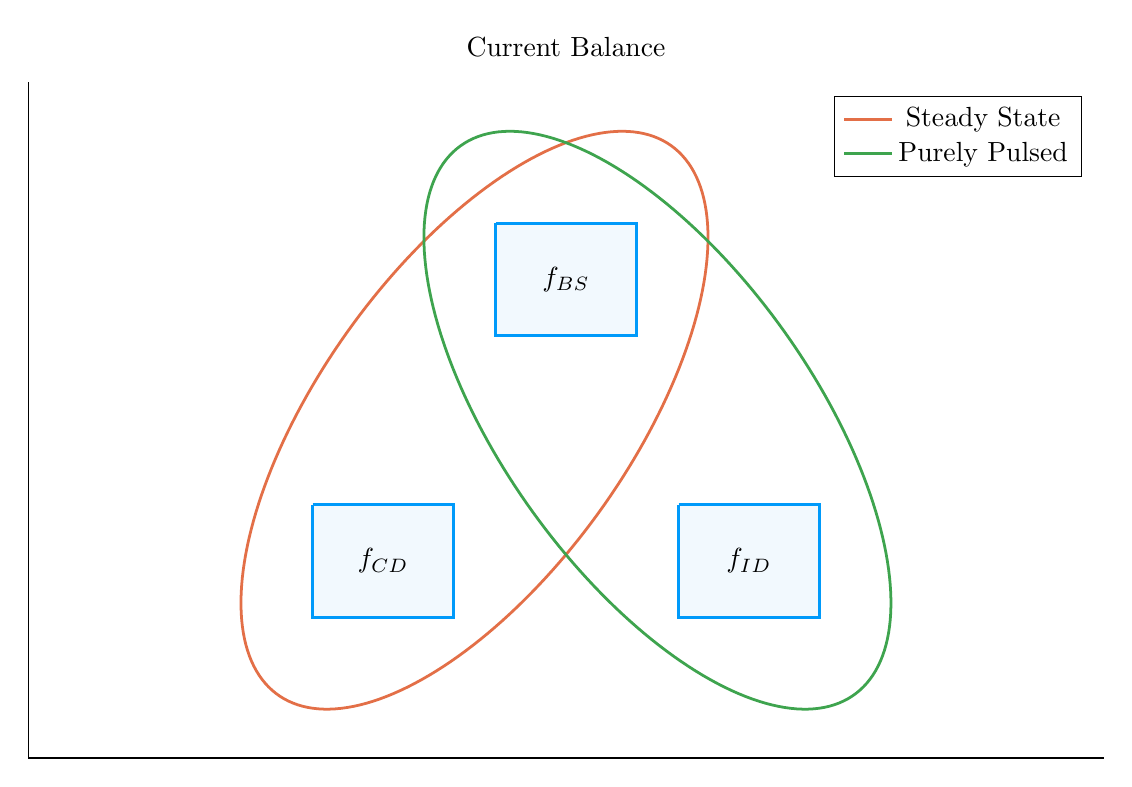
\begin{tikzpicture}[]
\begin{axis}[height = {101.6mm}, axis equal = {true}, ylabel = {}, title = {Current Balance}, xmin = {-5.773116112756781}, xmax = {5.773116112756781}, ymax = {6}, xlabel = {}, {unbounded coords=jump, scaled x ticks = false, xticklabel style={rotate = 0}, xmajorticks=false, xmajorgrids = false, axis lines* = left, scaled y ticks = false, yticklabel style={rotate = 0}, ymajorticks=false, ymajorgrids = false, axis lines* = left,     xshift = 0.0mm,
    yshift = 0.0mm,
    axis background/.style={fill={rgb,1:red,1.00000000;green,1.00000000;blue,1.00000000}}
}, ymin = {-6}, width = {152.4mm}]\addplot+ [color = {rgb,1:red,0.00000000;green,0.60560316;blue,0.97868012},
draw opacity=1.0,
line width=1,
solid,mark = none,
mark size = 2.0,
mark options = {
    color = {rgb,1:red,0.00000000;green,0.00000000;blue,0.00000000}, draw opacity = 1.0,
    fill = {rgb,1:red,0.00000000;green,0.60560316;blue,0.97868012}, fill opacity = 1.0,
    line width = 1,
    rotate = 0,
    solid
},fill = {rgb,1:red,0.00000000;green,0.60560316;blue,0.97868012}, fill opacity=0.05,forget plot]coordinates {
(-1.25, 3.5)
(1.25, 3.5)
(1.25, 1.5)
(-1.25, 1.5)
(-1.25, 3.5)
};
\addplot+ [color = {rgb,1:red,0.00000000;green,0.60560316;blue,0.97868012},
draw opacity=1.0,
line width=1,
solid,mark = none,
mark size = 2.0,
mark options = {
    color = {rgb,1:red,0.00000000;green,0.00000000;blue,0.00000000}, draw opacity = 1.0,
    fill = {rgb,1:red,0.00000000;green,0.60560316;blue,0.97868012}, fill opacity = 1.0,
    line width = 1,
    rotate = 0,
    solid
},fill = {rgb,1:red,0.00000000;green,0.60560316;blue,0.97868012}, fill opacity=0.05,forget plot]coordinates {
(-4.5, -1.5)
(-2.0, -1.5)
(-2.0, -3.5)
(-4.5, -3.5)
(-4.5, -1.5)
};
\addplot+ [color = {rgb,1:red,0.00000000;green,0.60560316;blue,0.97868012},
draw opacity=1.0,
line width=1,
solid,mark = none,
mark size = 2.0,
mark options = {
    color = {rgb,1:red,0.00000000;green,0.00000000;blue,0.00000000}, draw opacity = 1.0,
    fill = {rgb,1:red,0.00000000;green,0.60560316;blue,0.97868012}, fill opacity = 1.0,
    line width = 1,
    rotate = 0,
    solid
},fill = {rgb,1:red,0.00000000;green,0.60560316;blue,0.97868012}, fill opacity=0.05,forget plot]coordinates {
(2.0, -1.5)
(4.5, -1.5)
(4.5, -3.5)
(2.0, -3.5)
(2.0, -1.5)
};
\addplot+ [color = {rgb,1:red,0.88887350;green,0.43564919;blue,0.27812294},
draw opacity=1.0,
line width=1,
solid,mark = none,
mark size = 2.0,
mark options = {
    color = {rgb,1:red,0.00000000;green,0.00000000;blue,0.00000000}, draw opacity = 1.0,
    fill = {rgb,1:red,0.88887350;green,0.43564919;blue,0.27812294}, fill opacity = 1.0,
    line width = 1,
    rotate = 0,
    solid
}]coordinates {
(1.8698661812068136, 4.877080107549691)
(1.7975582266118808, 4.9252162522328415)
(1.7218385915440537, 4.9684428342438745)
(1.6427827549822935, 5.006716764385765)
(1.5604695215037632, 5.03999989037258)
(1.4749809427297138, 5.068259034860505)
(1.3864022355346433, 5.091466028519745)
(1.2948216971002622, 5.109597738114323)
(1.2003306168989445, 5.122636089561793)
(1.1030231856943935, 5.130568085949879)
(1.0029964016502424, 5.133385820492077)
(0.9003499736401737, 5.131086484409318)
(0.7951862218559462, 5.123672369729815)
(0.6876099758124048, 5.111150867004319)
(0.5777284698511354, 5.093534457939059)
(0.46565123624694493, 5.07084070295371)
(0.35148999602370634, 5.043092223676775)
(0.23535854758841435, 5.010316680395862)
(0.11737265329445545, 4.972546744485303)
(-0.00235007595282255, 4.929820065838624)
(-0.12369029793321751, 4.882179235338303)
(-0.2465270580745944, 4.829671742400261)
(-0.37073791002303214, 4.77234992763537)
(-0.49619903770001583, 4.710270930675205)
(-0.6227853787249911, 4.643496633214007)
(-0.7503707490802689, 4.572093597323671)
(-0.878827968893996, 4.496132999103221)
(-1.0080289892158198, 4.415690557728926)
(-1.137845019658864, 4.330846459975782)
(-1.26814665678079, 4.241685280285592)
(-1.3988040130759585, 4.148295896461316)
(-1.5296868464501256, 4.050771401071749)
(-1.6606646900485882, 3.949209008654826)
(-1.7916069823083864, 3.8437099588120507)
(-1.9223831971049103, 3.734379415290662)
(-2.0528629738631725, 3.6213263611541278)
(-2.1829162475040724, 3.5046634901454468)
(-2.3124133780960925, 3.3845070943515854)
(-2.4412252800831986, 3.26097694828099)
(-2.5692235509601344, 3.1341961894697543)
(-2.696280599266827, 3.004291195735447)
(-2.822269771774333, 2.8713914592009493)
(-2.947065479735527, 2.735629457213896)
(-3.0705433240746993, 2.597140520290374)
(-3.192580219391261, 2.4560626972145165)
(-3.3130545166539442, 2.3125366174284774)
(-3.4318461244632026, 2.166705350849943)
(-3.5488366287609345, 2.0187142652569277)
(-3.6639094108681878, 1.8687108813820061)
(-3.776949763733194, 1.7168447258604496)
(-3.8878450062738565, 1.5632671821788118)
(-3.9964845957006974, 1.4081313397725874)
(-4.1027602377083205, 1.2515918414233274)
(-4.206565994425528, 1.0938047291073505)
(-4.307798390016492, 0.9349272884497156)
(-4.4063565138277205, 0.7751178919384804)
(-4.502142120977991, 0.614535841055565)
(-4.595059730290983, 0.4533412074815748)
(-4.685016719472996, 0.29169467353285894)
(-4.771923417440856, 0.12975737198989234)
(-4.8556931937080146, -0.032309274523392384)
(-4.936242544739693, -0.1943437144491822)
(-5.013491177191022, -0.3561844283338884)
(-5.087362087945198, -0.5176700898342566)
(-5.157781640871865, -0.6786397265309694)
(-5.224679640229201, -0.8389328803894542)
(-5.287989400636577, -0.9983897677079463)
(-5.347647813547976, -1.1568514383933535)
(-5.403595410159981, -1.3141599344061687)
(-5.455776420691558, -1.4701584472164726)
(-5.504138829976595, -1.6246914741140965)
(-5.548634429313749, -1.7776049732170973)
(-5.589218864521925, -1.9287465170240605)
(-5.625851680153492, -2.0779654443571474)
(-5.658496359821148, -2.225113010544426)
(-5.687120362598258, -2.3700425356918093)
(-5.711695155456349, -2.5126095508967543)
(-5.732196241707455, -2.6526719422580065)
(-5.74860318542295, -2.7900900925378296)
(-5.760899631804527, -2.9247270203354994)
(-5.769073323487013, -3.0564485166333526)
(-5.773116112756781, -3.1851232785792454)
(-5.773023969673565, -3.3106230403720964)
(-5.768796986087595, -3.432822701120024)
(-5.760439375548035, -3.551600449543642)
(-5.747959469102832, -3.6668378854001826)
(-5.731369706994138, -3.778420137507439)
(-5.710686626257609, -3.8862359782498594)
(-5.685930844237935, -3.9901779344526522)
(-5.657127038037011, -4.090142394513381)
(-5.624303919915274, -4.186029711684261)
(-5.587494208670695, -4.2777443034022165)
(-5.546734597023965, -4.365194746567642)
(-5.502065715042401, -4.448293868676952)
(-5.453532089639006, -4.526958834718015)
(-5.4011821001870715, -4.601111229741906)
(-5.345067930294576, -4.67067713702862)
(-5.285245515786418, -4.735587211768881)
(-5.221774488946376, -4.795776750188546)
(-5.154718119074351, -4.851185754046737)
(-5.084143249418149, -4.901758990443393)
(-5.010120230542682, -4.947446046876624)
(-4.932722850202994, -4.98820138149499)
(-4.852028259791015, -5.023984368494613)
(-4.768116897429388, -5.054759338615853)
(-4.681072407788987, -5.080495614699213)
(-4.590981558710103, -5.101167542264987)
(-4.497934154710361, -5.116754515086211)
(-4.40202294746563, -5.127240995729401)
(-4.303343543353135, -5.132616531042591)
(-4.201994308148942, -5.132875762575277)
(-4.098076268974807, -5.1280184319198305)
(-3.9916930135921564, -5.118049380969083)
(-3.88295058714354, -5.102978547089826)
(-3.7719573864445346, -5.082820953217027)
(-3.658824051931438, -5.0575966928786364)
(-3.543663357372476, -5.02733091016593)
(-3.4265900974524626, -4.9920537746693245)
(-3.3077209733429527, -4.951800451404678)
(-3.1871744763719843, -4.906611065760036)
(-3.065070769909341, -4.8565306634977725)
(-2.941531569585093, -4.801609165851993)
(-2.816680021960811, -4.741901319765965)
(-2.690640581774395, -4.677466643319172)
(-2.5635388878808865, -4.608369366398399)
(-2.435501638012921, -4.5346783666719865)
(-2.306656462485676, -4.456467100931064)
(-2.1771317969721977, -4.373813531866238)
(-2.047056754475925, -4.286800050352669)
(-1.9165609966280504, -4.1955133933210735)
(-1.785774604437966, -4.100044557296444)
(-1.654827948625708, -4.00048870769076)
(-1.523851559665576, -3.896945083940012)
(-1.3929759976705065, -3.7895169005801836)
(-1.26233172224694, -3.678311244360763)
(-1.132048962449818, -3.5634389674983264)
(-1.0022575869674537, -3.4450145771766545)
(-0.8730869746655892, -3.323156121403477)
(-0.7446658856197179, -3.1979850713376368)
(-0.6171223327642645, -3.069626200204022)
(-0.49058345428648176, -2.938207458916877)
(-0.3651753868923626, -2.803859848535569)
(-0.24102314007082093, -2.666717289679875)
(-0.11825047148150092, -2.526916489034983)
(0.0030202364095237577, -2.384596803079324)
(0.12266809832327996, -2.2399000991709683)
(0.2405738466689491, -2.09297061413119)
(0.3566199504324037, -1.9439548104660527)
(0.4706907323336891, -1.7930012303693847)
(0.5826724841366269, -1.6402603476527216)
(0.6924535799956866, -1.4858844177497015)
(0.7999245877270309, -1.3300273259445707)
(0.9049783778929097, -1.1728444339759707)
(1.0075102305906167, -1.0144924251689658)
(1.1074179398395505, -0.8551291482497284)
(1.20460191546238, -0.6949134599984598)
(1.2989652823586764, -0.534005066897528)
(1.3904139770721349, -0.3725643659325606)
(1.478856841555075, -0.210752284705227)
(1.564205714036751, -0.04873012101713625)
(1.6463755169049392, 0.11334061791535466)
(1.725284341513138, 0.27529837645501054)
(1.8008535298288972, 0.4369817115859278)
(1.8730077528418523, 0.598229453843409)
(1.9416750856533156, 0.7588808679712085)
(2.0067870791725912, 0.9187758131459416)
(2.0682788283485025, 1.0777549026089095)
(2.126089036868173, 1.2356596625463219)
(2.1801600782585133, 1.3923326900594108)
(2.2304380533295443, 1.5476178100670777)
(2.2768728439022907, 1.7013602309846187)
(2.3194181627676604, 1.8534066990233193)
(2.358031599826549, 2.0036056509571933)
(2.392674664365143, 2.1518073652044736)
(2.423312823423304, 2.2978641110733555)
(2.4499155362177776, 2.4416302960231726)
(2.4724562845859026, 2.5829626107941834)
(2.490912599419497, 2.7217201722613846)
(2.505266083062553, 2.857764663869852)
(2.5155024276504205, 2.990960473511697)
(2.521611429372199, 3.12117482870718)
(2.5235869986421147, 3.2482779289551793)
(2.5214271661697554, 3.3721430751211794)
(2.515134084923101, 3.4926467957337035)
(2.5047140279823985, 3.609668970063368)
(2.4901773822870172, 3.7230929478618506)
(2.471538638281525, 3.8328056656413696)
(2.448816375471295, 3.9386977593788552)
(2.422033243902053, 4.040663673532358)
(2.391215941581816, 4.1386017662611385)
(2.356395187867742, 4.232414410744436)
(2.317605692844403, 4.322008092498024)
(2.274886122724018, 4.4072935025914814)
(2.2282790613031342, 4.488185626673267)
(2.1778309675141685, 4.564603829714885)
(2.123592129114139, 4.636471936389625)
(2.06561661255673, 4.70371830700579)
(2.0039622090976756, 4.766275908918702)
(1.9386903771871857, 4.824082383350291)
(1.869866181206814, 4.877080107549691)
};
\addlegendentry{Steady State}
\addplot+ [color = {rgb,1:red,0.24222430;green,0.64327509;blue,0.30444865},
draw opacity=1.0,
line width=1,
solid,mark = none,
mark size = 2.0,
mark options = {
    color = {rgb,1:red,0.00000000;green,0.00000000;blue,0.00000000}, draw opacity = 1.0,
    fill = {rgb,1:red,0.24222430;green,0.64327509;blue,0.30444865}, fill opacity = 1.0,
    line width = 1,
    rotate = 0,
    solid
}]coordinates {
(-1.8698661812068136, 4.877080107549691)
(-1.7975582266118808, 4.9252162522328415)
(-1.7218385915440537, 4.9684428342438745)
(-1.6427827549822935, 5.006716764385765)
(-1.5604695215037632, 5.03999989037258)
(-1.4749809427297138, 5.068259034860505)
(-1.3864022355346433, 5.091466028519745)
(-1.2948216971002622, 5.109597738114323)
(-1.2003306168989445, 5.122636089561793)
(-1.1030231856943935, 5.130568085949879)
(-1.0029964016502424, 5.133385820492077)
(-0.9003499736401737, 5.131086484409318)
(-0.7951862218559462, 5.123672369729815)
(-0.6876099758124048, 5.111150867004319)
(-0.5777284698511354, 5.093534457939059)
(-0.46565123624694493, 5.07084070295371)
(-0.35148999602370634, 5.043092223676775)
(-0.23535854758841435, 5.010316680395862)
(-0.11737265329445545, 4.972546744485303)
(0.00235007595282255, 4.929820065838624)
(0.12369029793321751, 4.882179235338303)
(0.2465270580745944, 4.829671742400261)
(0.37073791002303214, 4.77234992763537)
(0.49619903770001583, 4.710270930675205)
(0.6227853787249911, 4.643496633214007)
(0.7503707490802689, 4.572093597323671)
(0.878827968893996, 4.496132999103221)
(1.0080289892158198, 4.415690557728926)
(1.137845019658864, 4.330846459975782)
(1.26814665678079, 4.241685280285592)
(1.3988040130759585, 4.148295896461316)
(1.5296868464501256, 4.050771401071749)
(1.6606646900485882, 3.949209008654826)
(1.7916069823083864, 3.8437099588120507)
(1.9223831971049103, 3.734379415290662)
(2.0528629738631725, 3.6213263611541278)
(2.1829162475040724, 3.5046634901454468)
(2.3124133780960925, 3.3845070943515854)
(2.4412252800831986, 3.26097694828099)
(2.5692235509601344, 3.1341961894697543)
(2.696280599266827, 3.004291195735447)
(2.822269771774333, 2.8713914592009493)
(2.947065479735527, 2.735629457213896)
(3.0705433240746993, 2.597140520290374)
(3.192580219391261, 2.4560626972145165)
(3.3130545166539442, 2.3125366174284774)
(3.4318461244632026, 2.166705350849943)
(3.5488366287609345, 2.0187142652569277)
(3.6639094108681878, 1.8687108813820061)
(3.776949763733194, 1.7168447258604496)
(3.8878450062738565, 1.5632671821788118)
(3.9964845957006974, 1.4081313397725874)
(4.1027602377083205, 1.2515918414233274)
(4.206565994425528, 1.0938047291073505)
(4.307798390016492, 0.9349272884497156)
(4.4063565138277205, 0.7751178919384804)
(4.502142120977991, 0.614535841055565)
(4.595059730290983, 0.4533412074815748)
(4.685016719472996, 0.29169467353285894)
(4.771923417440856, 0.12975737198989234)
(4.8556931937080146, -0.032309274523392384)
(4.936242544739693, -0.1943437144491822)
(5.013491177191022, -0.3561844283338884)
(5.087362087945198, -0.5176700898342566)
(5.157781640871865, -0.6786397265309694)
(5.224679640229201, -0.8389328803894542)
(5.287989400636577, -0.9983897677079463)
(5.347647813547976, -1.1568514383933535)
(5.403595410159981, -1.3141599344061687)
(5.455776420691558, -1.4701584472164726)
(5.504138829976595, -1.6246914741140965)
(5.548634429313749, -1.7776049732170973)
(5.589218864521925, -1.9287465170240605)
(5.625851680153492, -2.0779654443571474)
(5.658496359821148, -2.225113010544426)
(5.687120362598258, -2.3700425356918093)
(5.711695155456349, -2.5126095508967543)
(5.732196241707455, -2.6526719422580065)
(5.74860318542295, -2.7900900925378296)
(5.760899631804527, -2.9247270203354994)
(5.769073323487013, -3.0564485166333526)
(5.773116112756781, -3.1851232785792454)
(5.773023969673565, -3.3106230403720964)
(5.768796986087595, -3.432822701120024)
(5.760439375548035, -3.551600449543642)
(5.747959469102832, -3.6668378854001826)
(5.731369706994138, -3.778420137507439)
(5.710686626257609, -3.8862359782498594)
(5.685930844237935, -3.9901779344526522)
(5.657127038037011, -4.090142394513381)
(5.624303919915274, -4.186029711684261)
(5.587494208670695, -4.2777443034022165)
(5.546734597023965, -4.365194746567642)
(5.502065715042401, -4.448293868676952)
(5.453532089639006, -4.526958834718015)
(5.4011821001870715, -4.601111229741906)
(5.345067930294576, -4.67067713702862)
(5.285245515786418, -4.735587211768881)
(5.221774488946376, -4.795776750188546)
(5.154718119074351, -4.851185754046737)
(5.084143249418149, -4.901758990443393)
(5.010120230542682, -4.947446046876624)
(4.932722850202994, -4.98820138149499)
(4.852028259791015, -5.023984368494613)
(4.768116897429388, -5.054759338615853)
(4.681072407788987, -5.080495614699213)
(4.590981558710103, -5.101167542264987)
(4.497934154710361, -5.116754515086211)
(4.40202294746563, -5.127240995729401)
(4.303343543353135, -5.132616531042591)
(4.201994308148942, -5.132875762575277)
(4.098076268974807, -5.1280184319198305)
(3.9916930135921564, -5.118049380969083)
(3.88295058714354, -5.102978547089826)
(3.7719573864445346, -5.082820953217027)
(3.658824051931438, -5.0575966928786364)
(3.543663357372476, -5.02733091016593)
(3.4265900974524626, -4.9920537746693245)
(3.3077209733429527, -4.951800451404678)
(3.1871744763719843, -4.906611065760036)
(3.065070769909341, -4.8565306634977725)
(2.941531569585093, -4.801609165851993)
(2.816680021960811, -4.741901319765965)
(2.690640581774395, -4.677466643319172)
(2.5635388878808865, -4.608369366398399)
(2.435501638012921, -4.5346783666719865)
(2.306656462485676, -4.456467100931064)
(2.1771317969721977, -4.373813531866238)
(2.047056754475925, -4.286800050352669)
(1.9165609966280504, -4.1955133933210735)
(1.785774604437966, -4.100044557296444)
(1.654827948625708, -4.00048870769076)
(1.523851559665576, -3.896945083940012)
(1.3929759976705065, -3.7895169005801836)
(1.26233172224694, -3.678311244360763)
(1.132048962449818, -3.5634389674983264)
(1.0022575869674537, -3.4450145771766545)
(0.8730869746655892, -3.323156121403477)
(0.7446658856197179, -3.1979850713376368)
(0.6171223327642645, -3.069626200204022)
(0.49058345428648176, -2.938207458916877)
(0.3651753868923626, -2.803859848535569)
(0.24102314007082093, -2.666717289679875)
(0.11825047148150092, -2.526916489034983)
(-0.0030202364095237577, -2.384596803079324)
(-0.12266809832327996, -2.2399000991709683)
(-0.2405738466689491, -2.09297061413119)
(-0.3566199504324037, -1.9439548104660527)
(-0.4706907323336891, -1.7930012303693847)
(-0.5826724841366269, -1.6402603476527216)
(-0.6924535799956866, -1.4858844177497015)
(-0.7999245877270309, -1.3300273259445707)
(-0.9049783778929097, -1.1728444339759707)
(-1.0075102305906167, -1.0144924251689658)
(-1.1074179398395505, -0.8551291482497284)
(-1.20460191546238, -0.6949134599984598)
(-1.2989652823586764, -0.534005066897528)
(-1.3904139770721349, -0.3725643659325606)
(-1.478856841555075, -0.210752284705227)
(-1.564205714036751, -0.04873012101713625)
(-1.6463755169049392, 0.11334061791535466)
(-1.725284341513138, 0.27529837645501054)
(-1.8008535298288972, 0.4369817115859278)
(-1.8730077528418523, 0.598229453843409)
(-1.9416750856533156, 0.7588808679712085)
(-2.0067870791725912, 0.9187758131459416)
(-2.0682788283485025, 1.0777549026089095)
(-2.126089036868173, 1.2356596625463219)
(-2.1801600782585133, 1.3923326900594108)
(-2.2304380533295443, 1.5476178100670777)
(-2.2768728439022907, 1.7013602309846187)
(-2.3194181627676604, 1.8534066990233193)
(-2.358031599826549, 2.0036056509571933)
(-2.392674664365143, 2.1518073652044736)
(-2.423312823423304, 2.2978641110733555)
(-2.4499155362177776, 2.4416302960231726)
(-2.4724562845859026, 2.5829626107941834)
(-2.490912599419497, 2.7217201722613846)
(-2.505266083062553, 2.857764663869852)
(-2.5155024276504205, 2.990960473511697)
(-2.521611429372199, 3.12117482870718)
(-2.5235869986421147, 3.2482779289551793)
(-2.5214271661697554, 3.3721430751211794)
(-2.515134084923101, 3.4926467957337035)
(-2.5047140279823985, 3.609668970063368)
(-2.4901773822870172, 3.7230929478618506)
(-2.471538638281525, 3.8328056656413696)
(-2.448816375471295, 3.9386977593788552)
(-2.422033243902053, 4.040663673532358)
(-2.391215941581816, 4.1386017662611385)
(-2.356395187867742, 4.232414410744436)
(-2.317605692844403, 4.322008092498024)
(-2.274886122724018, 4.4072935025914814)
(-2.2282790613031342, 4.488185626673267)
(-2.1778309675141685, 4.564603829714885)
(-2.123592129114139, 4.636471936389625)
(-2.06561661255673, 4.70371830700579)
(-2.0039622090976756, 4.766275908918702)
(-1.9386903771871857, 4.824082383350291)
(-1.869866181206814, 4.877080107549691)
};
\addlegendentry{Purely Pulsed}
\node at (axis cs:0, 2.5) [,
color={rgb,1:red,0.00000000;green,0.00000000;blue,0.00000000}, draw opacity=1.0,
rotate=0.0
] {$f_{BS}$};
\node at (axis cs:-3.25, -2.5) [,
color={rgb,1:red,0.00000000;green,0.00000000;blue,0.00000000}, draw opacity=1.0,
rotate=0.0
] {$f_{CD}$};
\node at (axis cs:3.25, -2.5) [,
color={rgb,1:red,0.00000000;green,0.00000000;blue,0.00000000}, draw opacity=1.0,
rotate=0.0
] {$f_{ID}$};
\end{axis}

\end{tikzpicture}

	\end{adjustbox}
%	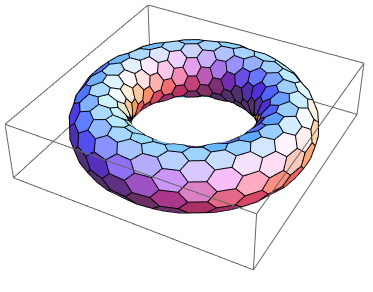
\includegraphics[width=0.75\textwidth]{images/test_image}
	\caption{Current Balance in a Tokamak} ~\\
	\small In a tokamak, there needs to be a certain amount of current -- and that current has to come from somewhere. All good reactors have an adequate bootstrap current. What provides the remaining current is what distinguishes steady state from pulsed operation.
	\label{fig:curbal}
\end{figure}

\subsubsection{The Tokamak Magnet Strength -- $B_0$}

The tokamak magnet strength has no \replaced{unique}{obvious} equation to eliminate it. With foresight, the one this model \replaced{uses}{chooses to use} is \added{the} power balance \replaced{inherent to every}{in a} reactor. Similar to current balance, power balance is what separates a reactor from a \replaced{device incapable of producing net electricity}{toaster}. As such, it is referred throughout this document as: the primary constraint. It will be derived later this chapter.

\subsubsection{The Tokamak Major Radius -- $R_0$}

Much like the magnet strength, the major radius has no \replaced{unique}{obvious} relation to express it. \replaced{The model therefore uses this equation to handle a reactor's various}{This is convenient, because the model still has yet to resolve one of its most pressing issues:} physical and engineering-based constraints. This \deleted{laundry} list of requirements further restricts reactor space to the curves shown in the results section. Collectively, these are referred to as the \replaced{limiting}{secondary} constraints -- discussed later this chapter. \replaced{These}{By miracle, these} constraints all just happen to depend on the size of the reactor -- the reason they are chosen to \replaced{represent}{substitute out} the radius.

\section{Enforcing Power Balance}

What separates a reactor from a \replaced{device incapable of producing net electricity}{toaster} is power balance. \replaced{Within a tokamak, it}{It} accounts for how the power going into a plasma's core exactly matches the power coming out of it. To approximate this conservation equation, two sets of power will be introduced: the sources and the sinks.

The sources have mainly been introduced at this point -- they include the alpha power ($P_\alpha$) \added{from fusion reactions} and the heating power ($P_H$), as well as a new ohmic power term ($P_\Omega$). The remaining two powers -- the sinks -- then appear through the radiation and heat conduction losses, which will be given shortly. In equation form, power balance becomes:
\begin{equation}
	\sum_{sources} P = \sum_{sinks} \, P
\end{equation}
or expanded to fit this model:
\begin{equation}
	\label{eq:power_balance}
	\tcboxmath{
	P_\alpha + P_H + P_\Omega = P_{BR} + P_\kappa
	}
\end{equation}
\myequations{Power Balance -- $P$}
For clarity, the left-hand side of this equality are the sources. Whereas the remaining two are sinks, i.e.\ Bremsstrahlung radiation ($P_{BR}$) and heat conduction losses ($P_\kappa$).

\subsection{Collecting Power Sources}

As suggested, the two dominant sources of power in a tokamak are: alpha power ($P_\alpha$) and auxiliary heating ($P_H$). From \cref{chapter:power}, it was determined that alpha particles (i.e.\ helium nuclei) carry around 20\% of the total fusion power; or as we put it mathematically:
\begin{equation}
	\tag{\ref{eq:palpha}}
	P_\alpha = \frac{P_F}{5}
\end{equation}
Additionally, it was determined that the heating power is what was eventually amplified into fusion power -- or through equation:
\begin{equation}
	\tag{\ref{eq:ph}}
	P_H = \frac{P_F}{Q}
\end{equation}
The final source term then is the ohmic power ($P_\Omega$). This is identical to how copper wires in a home heat up as current runs through them. From a simple circuits picture, the power across the plasma is related to its current and resistance -- in our standardized units -- through:\cite{process}
\begin{equation}
	\label{eq:pohmic_basic}
	P_\Omega = 10^6 \cdot I_P^2 \cdot R_P
\end{equation}
\replaced{This}{Here, the resistance of the plasma is unlike any material humans encounter on a daily basis -- actually decreasing with temperature. The} fusion systems model handles the plasma resistance ($R_P$)  with the neoclassical Spitzer resistivity. Through equation,\added{\cite{jeff}}
\begin{equation}
	\label{eq:rp}
	\tcbhighmath{
	R_P = \frac{K_{RP}}{R_0 \overline T ^ {3/2}}
	}
\end{equation}
\myequations{Plasma Resistance -- $R_P$}
\begin{equation}
	K_{RP} = 5.6e{-8} \cdot \left( \frac{ Z_{eff} }{ \epsilon^2 \kappa } \right) \cdot \left( \frac{1}{ 1 - 1.31 \sqrt{ \epsilon } + 0.46 \epsilon } \right)
\end{equation}
Combined with the Greenwald limit, ohmic power can be written more compactly as,
\begin{equation}
	\label{eq:pohmic}
	\tcboxmath{
	P_\Omega = K_\Omega \cdot \left( \frac{ \overline n ^ 2 R_0^3 }{\overline T ^ {3/2}} \right)
	}
\end{equation}
\myequations{Ohmic Power -- $P_\Omega$}
\begin{equation}
	K_\Omega = 10^6 \cdot \frac{K_{RP}}{K_n^2}
\end{equation}
With the sources defined, we are now in a position to discuss the two sink terms used in this model's power balance.

\subsection{Approximating Radiation Losses}

All nuclear reactors emit radiation. From a power balance perspective, this means some power has to always be reserved to recoup from its losses -- measured in megawatts. In a fusion reactor, the three most important types of radiation are: Bremsstrahlung radiation, line radiation, and synchrotron radiation.

\replaced{This}{Without going into too much detail, this} model chooses to only model Bremsstrahlung radiation -- as it usually dominates within the plasma's core. \added{Within most designs, Bremsstrahlung radiation outweighs the other two's contribution, to core power balance, two-to-one.\cite{ussteady,inputfile} } However, adding the effects of line-radiation and synchrotron radiation would drive results closer to real-world experiments. For example, line-radiation would better account for the \added{effects of} heavy impurities that \replaced{are emitted from the divertor plate and first wall}{appear as pieces of a tokamak fall into the plasma.}

For clarity, Bremsstrahlung -- or braking -- radiation is what occurs when a charged particle (e.g.\ an electron) is accelerated by some means. In a tokamak, this happens all the time as \replaced{electrons collide with the ion species.\cite{hutch}}{charged particles are flung around and around the machine.} \replaced{This term can be}{As given in Jeff Freidberg's book, this term is} described by the volume integral:\added{\cite{jeff}}
\begin{equation}
	P_{BR} = \int S_{BR} \ d \vec{\,r}
\end{equation}
\replaced{Where}{Here,} the radiation power density ($S_{BR}$) is given by:
\begin{equation}
	S_{BR} = \left( \frac{\sqrt{2}}{3 \sqrt{\pi^5}} \cdot \frac{e^6}{\epsilon_0^2 c^3 h m_e^{3/2}} \right) \cdot \left( Z_{eff} \, n^2 \, T^{1/2} \right)
\end{equation}
The constants in the left set of parentheses all have their usual physics meanings (i.e.\ c is the speed of light and $m_e$ is the mass of an electron). What is new is the effective charge: $Z_{eff}$.\cite{jeff}
\begin{equation}
	Z_{eff} = \frac{1}{n_e} \sum_j n_j Z_j^2
\end{equation}
The effective charge is a scheme for \replaced{reducing}{collapsing} the charge \replaced{each ion}{that each particle} has to a \replaced{single representative}{collective} value. Fundamental charge, here, is what: neutrons lack, electrons and hydrogen have one of, and helium has two. As such, a plasma with a purely deuterium and tritium fuel would have an effective charge of one. This value would then quickly rise if a Tungsten tile -- with 74 units of charge -- were to fall into the plasma core from the walls of the tokamak.\footnote{Typical effective charges ($Z_{eff}$) for a reactor are expected to be between 1 and 3.\cite{ussteady,inputfile,arc}} 

Using the volume integral -- seen in the derivation of fusion power -- allows the Bremsstrahlung power to be written in standardized units as:
\begin{equation}
	\label{eq:pbr}
	\tcboxmath{
	P_{BR} = K_{BR} \ \overline n ^ 2 \ \overline T ^ {1/2} R_0^3
	}
\end{equation}
\myequations{Bremsstrahlung Power -- $P_{BR}$}
\begin{equation}
	K_{BR} = 0.1056 \, \frac{ (1+\nu_n)^2 \, (1+\nu_T)^{1/2} }{1+2 \, \nu_n + 0.5 \, \nu_T} \, Z_{eff} \, \epsilon^2 \, \kappa \, g
\end{equation}

This power term represents the radiation power losses involved in power balance. All that is needed now is a formula for heat conduction losses -- \replaced{one of the most difficult plasma behaviors}{the hardest plasma behavior} to model to date.

\subsection{Estimating Heat Conduction Losses}

Heat is energy that \replaced{moves about randomly}{lacks direction} on a microscopic level. Macroscopically, it generally moves from hotter areas to colder ones. As hinted by the plasma profile for temperature, heat emanates from the center of a plasma and migrates towards the walls of its tokamak enclosure. It therefore \replaced{is a critical}{seems an important} quantity to calculate when balancing power in a plasma's core.

The difficulty of estimating heat conduction, though, lies in the \replaced{nonlinear behaviors}{chaotic nature} of plasmas -- no quick-running computation today can properly model it. As such, reactor designers have turned towards experimentalists for empirical scaling laws based on the dozen or so strongest tokamaks in the world. These are collectively referred to as confinement time scalings, i.e.\ the ELMy H-Mode Scaling Law.

The derivation of this heat conduction loss term ($P_\kappa$) starts in a manner similar to the previous powers. To begin, an equation for $P_\kappa$ \replaced{can be found using the following volume integral:\cite{jeff}}{sis given in Jeff Freidberg's book as:}
\begin{equation}
	P_\kappa = \frac{1}{\tau_E} \int U d \vec r
\end{equation}

This volume integral includes two new terms: the confinement time ($\tau_E$) and the internal energy (U). Before explaining these terms, a qualitative description is in order. As mentioned previously, the heat -- or microscopically random -- energy is captured by the internal energy (U). Then the confinement time ($\tau_E$) is how long it would take for the heat to \replaced{undergo an e-folding}{completely leave the device} if the \replaced{device}{system} were suddenly turned off.

A formula for confinement time will be delayed till the end of this section, when it is needed to solve for the magnetic field ($B_0$). The internal energy (U), however, can be given now as it has its typical physics meaning. This assumes that all three plasma species are held nearly at the same temperature (T) as the electrons:
\begin{equation}
	U = \frac{3}{2} \left( n + n_D + n_T \right) T
\end{equation}
Here again, $n_D$ and $n_T$ -- the density of deuterium and tritium, respectively -- are related to the electron density (used in this model) through the dilution factor, which assumes a 50-50 mix of D-T fuel:
\begin{equation}
	n_D = n_T = f_D \cdot \left( \, \frac{n}{2} \, \right)
\end{equation}
\replaced{After several substitutions,}{Foregoing the mathematical rigor of previous sections,} the equations here can be combined to form an equation for $P_\kappa$ -- the heat conduction losses -- in standardized units:
\begin{equation}
	\label{eq:pkappa}
	\tcboxmath{
	P_\kappa = K_\kappa \, \frac{ R_0 ^ 3 \ \overline{n}  \ \overline{T}  }{\tau_E}
	}
\end{equation}
\myequations{Heat Conduction Losses -- $P_\kappa$}
\begin{equation}
	K_\kappa = 0.4744 \, ( 1 + f_D ) \, \frac{ (1 + \nu_n) \, (1 + \nu_T) }{1 + \nu_n + \nu_T } \, ( \, \epsilon^2 \, \kappa \, g \, )
\end{equation}

Now that all five terms have been defined in power balance, the next step is expanding it and solving for the tokamak's toroidal magnetic field strength: $B_0$.

\subsection{Writing the Lawson \replaced{Parameter}{Criterion}}

Before \replaced{arriving at a formula for}{locking in the primary constraint -- i.e.\ } the magnet strength ($B_0$) \replaced{using}{equation from} power \replaced{balance,}{balance} -- it seems appropriate to take a detour and explain an intermediate solution: the Lawson \replaced{Parameter}{Criterion}.\cite{lawson} Within the fusion community, the Lawson \replaced{Parameter}{Criterion} is the cornerstone in any argument on the possibility of a \replaced{tokamak ever}{design} being used as a \replaced{reactor.}{reactor (and not just some grandiose toaster).}

An equation for the Lawson \replaced{Parameter}{Criterion} -- sometimes referred to as the \emph{triple product} -- is easily found in the literature as:\cite{jeff}
\begin{equation}
	\label{eq:lawson}
	n \cdot T \cdot \tau_E = \frac{ 60 }{ E_F } \cdot \frac{ T ^ 2 }{ \langle \sigma v \rangle }
\end{equation}
Similar to the steady current derived earlier, the right-hand side is only dependent on temperature. Further, as the left-hand side is a measure of difficult to achieve parameters, the goal is to minimize both sides. \replaced{As shown in \cref{fig:lawson}, this}{This} occurs when the plasma temperature is around 15 keV -- a fact \replaced{well known to}{memorized by} many fusion engineers. As will be seen, this is a simplified result of our model. This is why $\overline T$ = 15 keV is not always the optimum temperature -- but usually is in the right neighborhood for reasonable reactor designs.

\begin{figure}
	\centering
	\begin{adjustbox}{width=0.75\textwidth}
		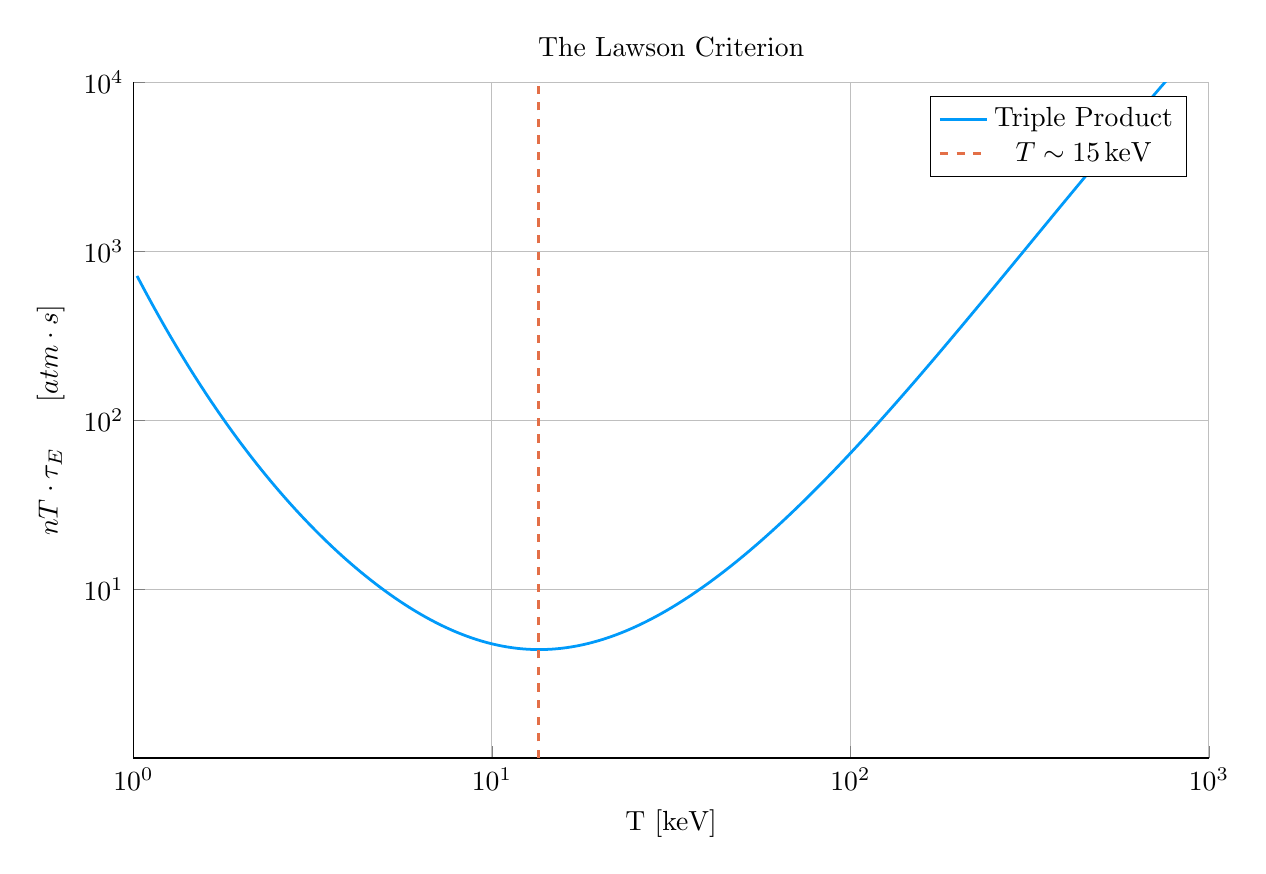
\begin{tikzpicture}[]
\begin{axis}[height = {101.6mm}, ylabel = {$n T \cdot \tau_E \ \ \ \ \ [atm \cdot s]$}, title = {The Lawson Criterion}, xmin = {1.0}, xmax = {1000.0}, ymax = {10000.0}, ymode = {log}, xlabel = {T   [keV]}, {unbounded coords=jump, xticklabel style={rotate = 0}, log basis x=10, xmajorgrids = true, xtick = {1.0,10.0,100.0,1000.0}, xticklabels = {$10^{0}$,$10^{1}$,$10^{2}$,$10^{3}$}, xtick align = inside, axis lines* = left, yticklabel style={rotate = 0}, log basis y=10, ymajorgrids = true, ytick = {10.0,100.0,1000.0,10000.0}, yticklabels = {$10^{1}$,$10^{2}$,$10^{3}$,$10^{4}$}, ytick align = inside, axis lines* = left,     xshift = 0.0mm,
    yshift = 0.0mm,
    axis background/.style={fill={rgb,1:red,1.00000000;green,1.00000000;blue,1.00000000}}
}, xmode = {log}, ymin = {1.001}, width = {152.4mm}]\addplot+ [color = {rgb,1:red,0.00000000;green,0.60560316;blue,0.97868012},
draw opacity=1.0,
line width=1,
solid,mark = none,
mark size = 2.0,
mark options = {
    color = {rgb,1:red,0.00000000;green,0.00000000;blue,0.00000000}, draw opacity = 1.0,
    fill = {rgb,1:red,0.00000000;green,0.60560316;blue,0.97868012}, fill opacity = 1.0,
    line width = 1,
    rotate = 0,
    solid
}]coordinates {
(1.023292992280754, 715.5843693055245)
(1.0471285480508996, 652.0764819850596)
(1.0715193052376064, 594.8592282501459)
(1.096478196143185, 543.2546522451097)
(1.1220184543019633, 496.663131536487)
(1.1481536214968828, 454.5537705698688)
(1.1748975549395295, 416.456035426309)
(1.202264434617413, 381.9524618339787)
(1.2302687708123816, 350.67229211863474)
(1.2589254117941673, 322.2859170225961)
(1.288249551693134, 296.50001561571264)
(1.318256738556407, 273.0533013093717)
(1.3489628825916535, 251.71279464231827)
(1.3803842646028848, 232.27055435304894)
(1.4125375446227544, 214.54080755655357)
(1.4454397707459274, 198.35742783107645)
(1.4791083881682074, 183.57171688596867)
(1.5135612484362082, 170.05045138851656)
(1.5488166189124815, 157.67416161454238)
(1.5848931924611136, 146.33561297294165)
(1.62181009735893, 135.9384652384002)
(1.6595869074375607, 126.3960875950959)
(1.6982436524617444, 117.63051042010802)
(1.7378008287493754, 109.57149718083319)
(1.7782794100389228, 102.155721939162)
(1.8197008586099834, 95.32603979193581)
(1.8620871366628675, 89.03083917128589)
(1.9054607179632472, 83.22346631314609)
(1.9498445997580451, 77.86171340616474)
(1.9952623149688795, 72.90736298097448)
(2.041737944669529, 68.32578201236458)
(2.0892961308540396, 64.08556000253319)
(2.137962089502232, 60.158186007840044)
(2.1877616239495525, 56.51776017780416)
(2.2387211385683394, 53.14073590510077)
(2.290867652767773, 50.0056891489945)
(2.344228815319922, 47.093111900666955)
(2.3988329190194904, 44.38522711472284)
(2.4547089156850306, 41.86582274326229)
(2.51188643150958, 39.52010278288166)
(2.5703957827688635, 37.33455348568332)
(2.6302679918953817, 35.29682309703734)
(2.6915348039269156, 33.395613669101465)
(2.7542287033381663, 31.62058366316803)
(2.8183829312644537, 29.962260198507185)
(2.884031503126606, 28.411959932944896)
(2.9512092266663856, 26.961717673034713)
(3.019951720402016, 25.60422191119189)
(3.0902954325135905, 24.332756575143232)
(3.1622776601683795, 23.141148352912094)
(3.2359365692962827, 22.0237190255119)
(3.311311214825911, 20.975242300634317)
(3.3884415613920256, 19.990904694824255)
(3.4673685045253166, 19.066270059743925)
(3.548133892335755, 18.197247390865947)
(3.630780547701014, 17.380061594923447)
(3.715352290971725, 16.611226926240565)
(3.8018939632056115, 15.887522832148305)
(3.890451449942806, 15.205971974493213)
(3.9810717055349722, 14.563820218135483)
(4.073802778041127, 13.9585183986498)
(4.168693834703354, 13.387705700467096)
(4.265795188015927, 12.849194493696395)
(4.36515832240166, 12.340956493058842)
(4.466835921509632, 11.86111011596177)
(4.570881896148751, 11.407908928906801)
(4.677351412871983, 10.979731082327069)
(4.786300923226384, 10.575069643717114)
(4.897788193684462, 10.192523747682124)
(5.011872336272722, 9.830790489396893)
(5.1286138399136485, 9.4886574950276)
(5.248074602497725, 9.16499610901522)
(5.370317963702527, 8.858755143826464)
(5.495408738576246, 8.568955142911767)
(5.623413251903491, 8.29468311223238)
(5.7543993733715695, 8.035087679882023)
(5.88843655355589, 7.789374647081937)
(6.025595860743578, 7.556802897213308)
(6.165950018614822, 7.336680632605374)
(6.309573444801933, 7.1283619115573345)
(6.456542290346556, 6.931243460563939)
(6.606934480075959, 6.7447617389697925)
(6.760829753919817, 6.5683902353161425)
(6.918309709189364, 6.4016369764913525)
(7.079457843841379, 6.244042232468866)
(7.244359600749901, 6.095176400934137)
(7.413102413009175, 5.954638057478739)
(7.5857757502918375, 5.822052158290098)
(7.762471166286917, 5.697068383402136)
(7.943282347242816, 5.579359609605691)
(8.128305161640993, 5.4686205030596)
(8.31763771102671, 5.364566222501177)
(8.511380382023766, 5.266931224738075)
(8.709635899560805, 5.175468164818683)
(8.912509381337454, 5.089946883932297)
(9.120108393559097, 5.010153478689247)
(9.33254300796991, 4.93588944597961)
(9.549925860214358, 4.866970898113729)
(9.772372209558107, 4.803227843409827)
(10.0, 4.74450352782116)
(10.232929922807541, 4.690653833587014)
(10.471285480508996, 4.641546731255455)
(10.715193052376065, 4.597061781760152)
(10.964781961431852, 4.557089685544928)
(11.220184543019636, 4.521531876017525)
(11.481536214968829, 4.490300154882151)
(11.748975549395297, 4.463316367150074)
(12.02264434617413, 4.4405121138606)
(12.302687708123818, 4.4218285007630715)
(12.589254117941675, 4.407215921415124)
(12.882495516931343, 4.39663387334517)
(13.182567385564074, 4.390050806109046)
(13.489628825916533, 4.38744400024263)
(13.803842646028846, 4.388799476276163)
(14.12537544622754, 4.3941119331320175)
(14.454397707459272, 4.403384715376948)
(14.791083881682072, 4.416629808943959)
(15.13561248436208, 4.433867865077917)
(15.488166189124811, 4.455128252393695)
(15.848931924611133, 4.48044913706814)
(16.218100973589298, 4.509877591315835)
(16.595869074375607, 4.5434697304270015)
(16.982436524617444, 4.581290878772013)
(17.378008287493753, 4.6234157653040935)
(17.78279410038923, 4.669928749218003)
(18.197008586099834, 4.72092407655112)
(18.620871366628677, 4.7765061686425785)
(19.054607179632473, 4.836789943498778)
(19.498445997580454, 4.9019011712485865)
(19.952623149688797, 4.971976865010962)
(20.417379446695296, 5.047165708641305)
(20.892961308540396, 5.127628522971638)
(21.379620895022324, 5.213538772314609)
(21.87761623949553, 5.305083113162599)
(22.3872113856834, 5.4024619871819475)
(22.908676527677734, 5.505890260779421)
(23.442288153199225, 5.615597913703399)
(23.9883291901949, 5.73183077933847)
(24.547089156850298, 5.854851339557513)
(25.118864315095795, 5.984939577213792)
(25.703957827688633, 6.122393889584756)
(26.302679918953814, 6.267532066323497)
(26.915348039269155, 6.420692335730828)
(27.542287033381662, 6.582234483434617)
(28.183829312644534, 6.752541047852738)
(28.84031503126606, 6.932018597123181)
(29.512092266663856, 7.121099092511616)
(30.19951720402016, 7.3202413436533345)
(30.902954325135905, 7.52993256135462)
(31.622776601683793, 7.750690014070107)
(32.359365692962825, 7.983062794588698)
(33.11311214825911, 8.227633703902626)
(33.884415613920254, 8.485021259704226)
(34.673685045253166, 8.75588183745494)
(35.48133892335755, 9.040911952501903)
(36.30780547701014, 9.340850692282585)
(37.15352290971726, 9.656482308258274)
(38.018939632056124, 9.988638977855283)
(38.90451449942807, 10.33820374737135)
(39.810717055349734, 10.706113667526031)
(40.73802778041128, 11.093363134099329)
(41.68693834703355, 11.50100744691819)
(42.65795188015925, 11.930166601314705)
(43.65158322401658, 12.382029327098968)
(44.6683592150963, 12.857857391065538)
(45.708818961487495, 13.358990180088743)
(46.77351412871981, 13.886849582961755)
(47.86300923226383, 14.442945190302456)
(48.97788193684461, 15.028879833087446)
(50.11872336272722, 15.646355481690618)
(51.28613839913648, 16.297179528695864)
(52.48074602497726, 16.983271480232325)
(53.70317963702527, 17.706670082146438)
(54.954087385762456, 18.469540908986364)
(56.23413251903491, 19.274184445531887)
(57.543993733715695, 20.1230446924667)
(58.8843655355589, 21.01871832976149)
(60.25595860743578, 21.963964473423015)
(61.65950018614822, 22.96171506347328)
(63.09573444801933, 24.015085923357283)
(64.56542290346556, 25.127388533447483)
(66.06934480075961, 26.302142563921986)
(67.60829753919819, 27.543089215049925)
(69.18309709189366, 28.85420541582856)
(70.79457843841381, 30.2397189349887)
(72.44359600749902, 31.704124461627565)
(74.13102413009177, 33.25220071614717)
(75.85775750291836, 34.889028655780834)
(77.62471166286916, 36.620010842788844)
(79.43282347242814, 38.45089204740532)
(81.2830516164099, 40.387781161829686)
(83.17637711026708, 42.43717450598852)
(85.11380382023764, 44.6059806104552)
(87.09635899560806, 46.90154656681403)
(89.12509381337455, 49.331686040906135)
(91.20108393559097, 51.90470904980014)
(93.3254300796991, 54.62945360900688)
(95.49925860214358, 57.515319362410956)
(97.72372209558107, 60.57230331363601)
(100.0, 63.81103778410115)
(102.32929922807536, 67.24283072987917)
(104.71285480508996, 70.87970855663967)
(107.1519305237606, 74.73446157946178)
(109.64781961431851, 78.82069228215158)
(112.2018454301963, 83.15286653889214)
(114.81536214968828, 87.74636796962139)
(117.48975549395291, 92.61755560946783)
(120.22644346174131, 97.78382508189834)
(123.02687708123811, 103.26367347494983)
(125.89254117941675, 109.07676813004912)
(128.82495516931337, 115.24401956346287)
(131.82567385564073, 121.78765875140567)
(134.89628825916532, 128.7313190212372)
(138.03842646028852, 136.10012280306256)
(141.2537544622754, 143.92077350836064)
(144.5439770745928, 152.22165281508785)
(147.91083881682073, 161.03292365197024)
(151.35612484362088, 170.38663918850096)
(154.88166189124811, 180.3168581514265)
(158.48931924611142, 190.859766803331)
(162.18100973589299, 202.05380793424246)
(165.95869074375614, 213.93981723308698)
(169.82436524617444, 226.5611674222155)
(173.78008287493762, 239.96392055525848)
(177.82794100389228, 254.19698889610504)
(181.97008586099827, 269.3123048150095)
(186.20871366628674, 285.3650001565748)
(190.54607179632464, 302.41359555379074)
(194.98445997580455, 320.5202001823509)
(199.52623149688787, 339.75072247016425)
(204.17379446695296, 360.175092298409)
(208.92961308540387, 381.86749525252964)
(213.79620895022325, 404.9066195044671)
(218.77616239495518, 429.37591593094083)
(223.872113856834, 455.36387209705316)
(229.08676527677724, 482.9643007596241)
(234.42288153199226, 512.2766435708044)
(239.88329190194898, 543.4062906894171)
(245.4708915685031, 576.464917035484)
(251.18864315095797, 611.5708359522358)
(257.03957827688646, 648.8493710699868)
(263.02679918953817, 688.4332471972791)
(269.1534803926917, 730.4630010970918)
(275.4228703338166, 775.087413039401)
(281.8382931264455, 822.4639600564246)
(288.40315031266056, 872.7592918631268)
(295.1209226666387, 926.1497304436313)
(301.9951720402016, 982.8217943436637)
(309.0295432513592, 1042.972748750622)
(316.22776601683796, 1106.8111824860716)
(323.5936569296281, 1174.5576130809143)
(331.1311214825911, 1246.4451211509213)
(338.84415613920237, 1322.7200153403764)
(346.73685045253166, 1403.6425291540393)
(354.8133892335753, 1489.4875510528248)
(363.0780547701014, 1580.545389247023)
(371.5352290971724, 1677.1225726820153)
(380.1893963205613, 1779.542689776586)
(389.04514499428046, 1888.147266542193)
(398.1071705534973, 2003.2966857842675)
(407.3802778041126, 2125.3711491630897)
(416.8693834703355, 2254.771683973346)
(426.57951880159254, 2391.92119658728)
(436.5158322401661, 2537.2655745980082)
(446.683592150963, 2691.2748397961623)
(457.0881896148752, 2854.4443542162185)
(467.73514128719813, 3027.296081597634)
(478.6300923226385, 3210.379906722357)
(489.77881936844614, 3404.2750152128565)
(501.18723362727246, 3609.591336506103)
(512.8613839913648, 3826.971052857308)
(524.8074602497728, 4057.0901773752544)
(537.0317963702527, 4300.660204247052)
(549.5408738576248, 4558.429834477045)
(562.341325190349, 4831.186780640399)
(575.4399373371566, 5119.759654339896)
(588.843655355589, 5425.019940252352)
(602.5595860743575, 5747.884060862276)
(616.5950018614822, 6089.315536203627)
(630.957344480193, 6450.327243166718)
(645.6542290346556, 6831.983779178804)
(660.6934480075957, 7235.403935331275)
(676.0829753919819, 7661.763284308377)
(691.8309709189363, 8112.296888768487)
(707.945784384138, 8588.302136144339)
(724.4359600749899, 9091.141706159546)
(741.3102413009177, 9622.24667771128)
(758.5775750291835, 10183.11978213795)
(776.247116628692, 10775.338810284076)
(794.3282347242813, 11400.560181185736)
(812.8305161640995, 12060.52268063764)
(831.7637711026708, 12757.051378360826)
(851.1380382023768, 13492.06173297636)
(870.9635899560806, 14267.563894499495)
(891.2509381337459, 15085.667214609008)
(912.0108393559096, 15948.584975511469)
(933.2543007969915, 16858.63934881972)
(954.992586021436, 17818.266596491703)
(977.2372209558112, 18830.022526540524)
(1000.0, 19896.588216921093)
(1023.2929922807537, 21020.77602173607)
(1047.1285480508996, 22205.535874673045)
(1071.519305237606, 23453.961905400487)
(1096.4781961431852, 24769.29938550517)
(1122.018454301963, 26154.952021453166)
(1148.1536214968828, 27614.489613007096)
(1174.897554939529, 29151.656096526574)
(1202.2644346174131, 30770.37799363245)
(1230.268770812381, 32474.77328681697)
(1258.9254117941675, 34269.16074474929)
(1288.2495516931335, 36158.06972124623)
(1318.2567385564075, 38146.2504531722)
(1348.9628825916532, 40238.68488388557)
(1380.3842646028852, 42440.598040283076)
(1412.537544622754, 44757.46999299408)
(1445.439770745928, 47195.048430870826)
(1479.1083881682073, 49759.3618825815)
(1513.5612484362086, 52456.73361988538)
(1548.816618912481, 55293.79627901266)
(1584.893192461114, 58277.5072385393)
(1621.8100973589299, 61415.16479419626)
(1659.5869074375614, 64714.42517323727)
(1698.2436524617442, 68183.3204332687)
(1737.8008287493763, 71830.27729287352)
(1778.2794100389228, 75664.13694389607)
(1819.7008586099826, 79694.17589795444)
(1862.0871366628676, 83930.12792257269)
(1905.4607179632462, 88382.20712532024)
(1949.8445997580454, 93061.13224750487)
(1995.2623149688789, 97978.15223228547)
(2041.7379446695295, 103145.07313560059)
(2089.296130854039, 108574.28645200086)
(2137.9620895022326, 114278.79893140584)
(2187.761623949552, 120272.26396692236)
(2238.72113856834, 126569.01463824147)
(2290.8676527677726, 133184.09849971998)
(2344.228815319923, 140133.3142071364)
(2398.83291901949, 147433.25008222583)
(2454.708915685031, 155101.32471954415)
(2511.88643150958, 163155.82974591767)
(2570.3957827688646, 171615.97484880453)
(2630.2679918953813, 180501.9351962624)
(2691.5348039269165, 189834.9013779866)
(2754.2287033381663, 199637.13200398907)
(2818.382931264455, 209932.00910503615)
(2884.031503126606, 220744.09648690396)
(2951.209226666387, 232099.20119892008)
(3019.9517204020162, 244024.43828613157)
(3090.295432513592, 256548.29900382337)
(3162.2776601683795, 269700.72268301074)
(3235.936569296281, 283513.1724460091)
(3311.311214825911, 298018.714982234)
(3388.441561392024, 313252.1046060778)
(3467.368504525317, 329249.87183106877)
(3548.133892335753, 346050.41670754453)
(3630.780547701014, 363694.1071848948)
(3715.352290971724, 382223.3827739712)
(3801.8939632056126, 401682.863800698)
(3890.4514499428046, 422119.46655815904)
(3981.0717055349733, 443582.52468168386)
(4073.802778041126, 466123.9170895939)
(4168.693834703355, 489798.2028515374)
(4265.795188015925, 514662.763366615)
(4365.158322401661, 540777.9522550126)
(4466.835921509631, 568207.2533895164)
(4570.881896148751, 597017.4475173334)
(4677.351412871981, 627278.7879479581)
(4786.300923226385, 659065.1858096905)
(4897.7881936844615, 692454.4054057244)
(5011.872336272725, 727528.2702307551)
(5128.613839913648, 764372.8802406823)
(5248.074602497728, 803078.841001585)
(5370.317963702527, 843741.5053794787)
(5495.408738576249, 886461.2284699624)
(5623.413251903491, 931343.6365063301)
(5754.399373371566, 978499.910526803)
(5888.43655355589, 1.0280470856256834e6)
(6025.595860743575, 1.080108366660198e6)
(6165.9500186148225, 1.1348134613343545e6)
(6309.57344480193, 1.1922989316334699e6)
(6456.542290346556, 1.252708564638612e6)
(6606.934480075957, 1.3161937638086632e6)
(6760.829753919818, 1.3829139618799328e6)
(6918.309709189362, 1.4530370565986685e6)
(7079.457843841381, 1.52673987057139e6)
(7244.359600749898, 1.6042086365912505e6)
(7413.102413009177, 1.6856395098764265e6)
(7585.775750291836, 1.771239108738555e6)
(7762.4711662869195, 1.8612250852863907e6)
(7943.282347242814, 1.955826727861547e6)
(8128.305161640995, 2.0552855970008024e6)
(8317.63771102671, 2.1598561968221436e6)
(8511.380382023768, 2.2698066838408946e6)
(8709.635899560806, 2.385419615337356e6)
(8912.509381337459, 2.506992739519579e6)
(9120.108393559096, 2.6348398298537624e6)
(9332.543007969914, 2.7692915660716193e6)
(9549.92586021436, 2.910696464508343e6)
(9772.372209558112, 3.0594218605781165e6)
(10000.0, 3.2158549463557494e6)
};
\addlegendentry{Triple Product}
\addplot+ [color = {rgb,1:red,0.88887350;green,0.43564919;blue,0.27812294},
draw opacity=1.0,
line width=1,
dashed,mark = none,
mark size = 2.0,
mark options = {
    color = {rgb,1:red,0.00000000;green,0.00000000;blue,0.00000000}, draw opacity = 1.0,
    fill = {rgb,1:red,0.88887350;green,0.43564919;blue,0.27812294}, fill opacity = 1.0,
    line width = 1,
    rotate = 0,
    solid
}]coordinates {
(13.489628825916533, 1.0)
(13.489628825916533, 10000.0)
};
\addlegendentry{$T \sim 15 \, \textnormal{keV}$}
\end{axis}

\end{tikzpicture}

	\end{adjustbox}
%	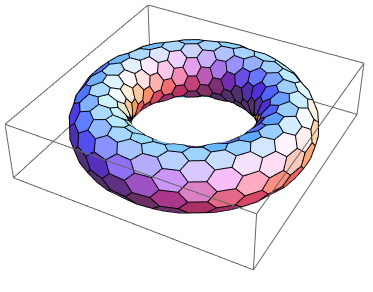
\includegraphics[width=0.75\textwidth]{images/test_image}
	\caption{Power Balance in a Reactor} ~\\
	\small Power balance is what differentiates a reactor from a net power loss experiment. When cast as the Lawson \replaced{Parameter}{Criterion} for fusion, it explains why D-T plasmas often have a temperature around 15 keV.
	\label{fig:lawson}
\end{figure}

As all the terms in power balance have already been defined, the starting point will be simply repeating the standardized equations for all five included powers.
\begin{gather}
	\tag{\ref{eq:palpha}}
	P_\alpha = \frac{P_F}{5} \\
	\tag{\ref{eq:ph}}
	P_H = \frac{P_F}{Q} \\
	\tag{\ref{eq:pohmic}}
	P_\Omega = K_\Omega \cdot \left( \frac{ \overline n ^ 2 R_0^3 }{\overline T ^ {3/2}} \right) \\
	\tag{\ref{eq:pbr}}
	P_{BR} = K_{BR} \ \overline n ^ 2 \ \overline T ^ {1/2} R_0^3 \\
	\tag{\ref{eq:pkappa}}
	P_\kappa = K_\kappa \, \frac{ R_0 ^ 3 \ \overline{n}  \ \overline{T}  }{\tau_E}
\end{gather}

With the fusion power again being,
\begin{equation}
	\tag{\ref{eq:pf}}
	P_F = K_F \cdot \overline{n}^2 \cdot R_0^3  \cdot (\sigma v)
\end{equation}
These can then be substituted into power balance:
\begin{equation}
	\tag{\ref{eq:power_balance}}
	P_\alpha + P_H + P_\Omega = P_{BR} + P_\kappa
\end{equation}
After a couple lines of algebra, power balance can be rewritten in a form analogous to the triple product:
\begin{equation}
	\label{eq:ntaue}
	\tcboxmath{
	 \overline{n}  \cdot \overline{T} \cdot \tau_E = \frac{ K_\kappa \, \overline{T}^{\,2} }{ \left( K_P \, (\sigma v) +  K_{OH} \, \overline{T}^{  \,-3/2 } \right) - K_{BR} \, \overline{T}^{  \,1/2 } }
	 }
\end{equation}
\myequations{Triple Product -- $\overline{n}  \cdot \overline{T} \cdot \tau_E$}
\begin{equation}
	K_P = K_F \cdot \left( \frac{5 + Q}{5 \times Q} \right)
\end{equation}
\replaced{As expected, this shares a form}{As can be seen, this is remarkably} similar to the simple Lawson \replaced{Parameter}{Criterion}:
\begin{equation}
	\tag{\ref{eq:lawson}}
	n \cdot T \cdot \tau_E = \frac{ 60 }{ E_F } \cdot \frac{ T ^ 2 }{ \langle \sigma v \rangle }
\end{equation}
The main difference is this model does not ignore ohmic power and radiation losses completely. The inclusion of radiation for example sometimes bars a range of temperatures from being physically realizable.\footnote{ The denominator of Eq \ref{eq:ntaue} has discontinuities when the $K_{BR} \, \overline{T}^{  \,1/2 }$ term exactly equals the parenthesised one. Therefore, valid reactors only exist outside the discontinuities, when the entire triple product is finite and positive. } With this intermediate relation in place, the goal is now to give a formula for the confinement time and solve it for the magnetic field strength ($B_0$) -- thus giving the Primary Constraint.

\subsection{Finalizing the Primary Constraint}

The goal now is to transform the Lawson \replaced{Parameter}{Criterion} into an equation for magnet strength ($B_0$). This choice to solve the equation for $B_0$ was \replaced{motivated by the goals of analysis and how it will fit}{completely arbitrary, only motivated by the foresight of how it fits} into the fusion systems model. To solve the primary constraint, the confinement time scaling law will need to be introduced. At the end, a \replaced{convoluted}{messy} -- albeit highly useful -- relation will be the reward.

\begin{figure}
	\centering
	\begin{adjustbox}{width=0.75\textwidth}
		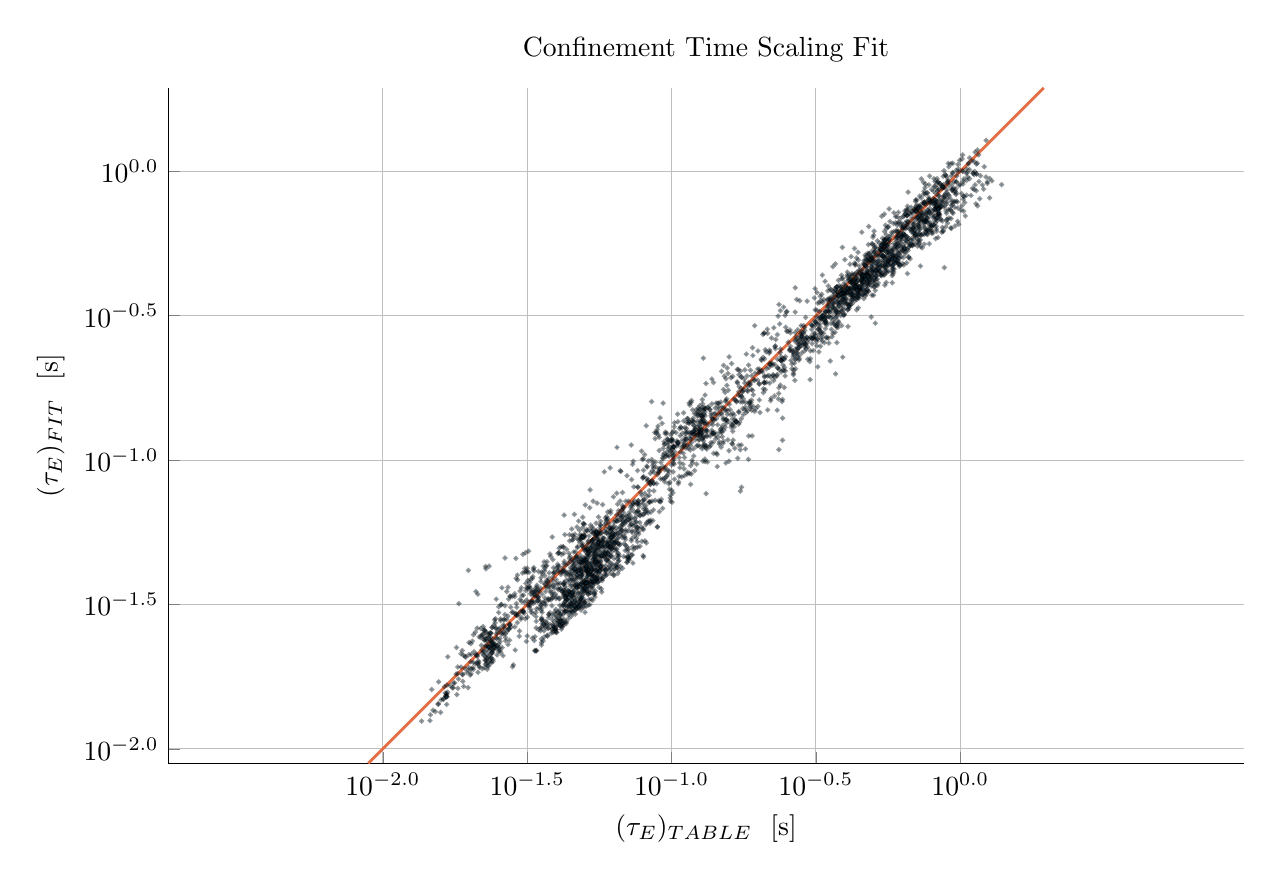
\begin{tikzpicture}[]
\begin{axis}[height = {101.6mm}, axis equal = {true}, ylabel = {$(\tau_E)_{ FIT } \ \ [ \textnormal{s} ]$}, title = {Confinement Time Scaling Fit}, xmin = {0.008904842990761705}, xmax = {1.9473999999999996}, ymax = {1.9473999999999996}, ymode = {log}, xlabel = {$(\tau_E)_{ TABLE } \ \ [ \textnormal{s} ]$}, {unbounded coords=jump, scaled x ticks = false, xticklabel style={rotate = 0}, log basis x=10, xmajorgrids = true, xtick = {0.01,0.03162277660168379,0.1,0.31622776601683794,1.0}, xticklabels = {$10^{-2.0}$,$10^{-1.5}$,$10^{-1.0}$,$10^{-0.5}$,$10^{0.0}$}, xtick align = inside, axis lines* = left, scaled y ticks = false, yticklabel style={rotate = 0}, log basis y=10, ymajorgrids = true, ytick = {0.01,0.03162277660168379,0.1,0.31622776601683794,1.0}, yticklabels = {$10^{-2.0}$,$10^{-1.5}$,$10^{-1.0}$,$10^{-0.5}$,$10^{0.0}$}, ytick align = inside, axis lines* = left,     xshift = 0.0mm,
    yshift = 0.0mm,
    axis background/.style={fill={rgb,1:red,1.00000000;green,1.00000000;blue,1.00000000}}
}, xmode = {log}, ymin = {0.008904842990761705}, width = {152.4mm}]\addplot+[draw=none, color = {rgb,1:red,0.00000000;green,0.60560316;blue,0.97868012},
draw opacity=0.4,
line width=0,
solid,mark = *,
mark size = 0.325,
mark options = {
    color = {rgb,1:red,0.00000000;green,0.00000000;blue,0.00000000}, draw opacity = 0.4,
    fill = {rgb,1:red,0.00000000;green,0.60560316;blue,0.97868012}, fill opacity = 0.4,
    line width = 1,
    rotate = 0,
    solid
},forget plot] coordinates {
(0.048709999999999996, 0.03286927009465151)
(0.047479999999999994, 0.030718782340371346)
(0.056709999999999997, 0.04427687673230967)
(0.06154, 0.040523205193333994)
(0.049249999999999995, 0.031000215657666388)
(0.046439999999999995, 0.03902384637413358)
(0.04536, 0.03366158264691253)
(0.041229999999999996, 0.029311430641277475)
(0.04224, 0.03489492877112558)
(0.05357, 0.03985677848149215)
(0.042449999999999995, 0.030139467297048302)
(0.04393, 0.03525642598465171)
(0.037579999999999995, 0.029115058174186102)
(0.040589999999999994, 0.03552938448965956)
(0.016339999999999997, 0.016414220556232706)
(0.01926, 0.018966660638066977)
(0.014769999999999998, 0.01604916788911629)
(0.020909999999999998, 0.019687625330862386)
(0.014559999999999998, 0.01252323235667468)
(0.016659999999999998, 0.016615842361327)
(0.017099999999999997, 0.016562775820865377)
(0.025429999999999998, 0.024119656293897448)
(0.01834, 0.03183654298531315)
(0.02225, 0.026522518089311862)
(0.02354, 0.023762954142859543)
(0.01883, 0.02190554572449257)
(0.0156, 0.0170549295762654)
(0.01678, 0.020822704009415233)
(0.154, 0.14943255990407037)
(0.17639999999999997, 0.1506224447310805)
(0.7525999999999999, 0.7841653529419872)
(0.7196999999999999, 0.7123510444198007)
(0.7581, 0.7126653992395249)
(0.5971, 0.6636747785042374)
(0.5545, 0.6034081737695671)
(0.5620999999999999, 0.5855426425362842)
(0.7231, 0.611757051674103)
(0.7314999999999999, 0.6000776436052295)
(0.8261999999999999, 0.7332080576221435)
(0.8526999999999999, 0.6874473851854792)
(0.7659999999999999, 0.6249854199535853)
(0.8212999999999999, 0.6647675128338589)
(0.7968, 0.6202645990011652)
(1.1369999999999998, 0.8572954951071405)
(0.8379, 0.709498458538988)
(0.7112999999999999, 0.6481476339591892)
(0.8383999999999999, 0.7100253242029977)
(0.9772, 0.7850517774047457)
(0.6932999999999999, 0.6449986085844157)
(0.7078, 0.5696128161569505)
(0.7666999999999999, 0.6076651618162499)
(0.7231, 0.8218656209469912)
(0.7654, 0.7824204839027497)
(0.8880999999999999, 0.9751544259782554)
(0.9436, 0.987045215482296)
(0.982, 1.0567556111003251)
(1.0659999999999998, 1.0600221351309262)
(1.021, 1.0023421135083617)
(1.037, 0.780421246365204)
(1.0139999999999998, 0.7598649860996711)
(0.9391999999999999, 0.722374477345195)
(0.7876, 0.7737488110528499)
(0.7564, 0.8355652777917266)
(0.8073999999999999, 0.7829615268340135)
(0.6101, 0.662119064106307)
(0.5015, 0.6015695673902948)
(0.7323999999999999, 0.8090796506003152)
(0.6535, 0.7394639493973881)
(0.5972, 0.6975536633839833)
(0.8778999999999999, 0.7874999827504517)
(0.7773, 0.8125562886500788)
(0.6810999999999999, 0.7238692523345119)
(0.6392, 0.701072652615907)
(0.6046999999999999, 0.6507248504722397)
(0.9085, 1.0662323587837632)
(0.746, 0.9171741777262944)
(0.6601999999999999, 0.8477587902173862)
(1.019, 1.1402820961295275)
(0.9123, 1.0371038527895822)
(0.5081, 0.5255375119481419)
(0.7402, 0.6843189302449205)
(0.7313999999999999, 0.6912025500896107)
(1.0779999999999998, 1.1138270195034614)
(0.6314, 0.6309700937894861)
(0.9303999999999999, 0.9647835607071941)
(0.8503, 0.9084098651600415)
(0.8125, 0.8871934724039697)
(0.9943, 1.0920838325900788)
(0.8109999999999999, 0.94316240550339)
(0.7583, 0.9027068941508603)
(0.8357, 0.9197400869136341)
(0.6762999999999999, 0.7509390530838264)
(0.6529999999999999, 0.7031904860947172)
(0.3892, 0.34318485870648646)
(0.34049999999999997, 0.3124029593731834)
(0.45299999999999996, 0.3908324185235881)
(0.44149999999999995, 0.37445805641759866)
(0.5680999999999999, 0.519309036063986)
(0.5427, 0.470258508275619)
(0.3973, 0.3208880474419727)
(0.4023, 0.3620545624474692)
(0.36279999999999996, 0.3723269788644909)
(0.5475, 0.4394327211967968)
(0.3898, 0.37922457801357046)
(0.31279999999999997, 0.303118325347936)
(0.38389999999999996, 0.35281373501460195)
(0.3181, 0.31386085182034285)
(0.7142, 0.6930925801653104)
(0.6252, 0.6626568011479417)
(0.6154999999999999, 0.5263153459242683)
(0.9141999999999999, 0.6902582143865932)
(0.7587999999999999, 0.6215886466745869)
(0.6337999999999999, 0.5997015869390643)
(0.9221999999999999, 0.7382203149764545)
(0.6928, 0.6177290812059213)
(0.7125999999999999, 0.6963967594591091)
(0.21899999999999997, 0.18496435234301067)
(0.20789999999999997, 0.1766203805469118)
(0.26499999999999996, 0.20490261922028621)
(0.4225, 0.34891440428748743)
(0.4118, 0.3421446077261888)
(0.2397, 0.22159945467095882)
(0.26959999999999995, 0.22409261472703068)
(0.3127, 0.2631427459860977)
(0.32389999999999997, 0.2832737570128158)
(0.8515999999999999, 0.9068928303444452)
(0.8177, 0.9220516908419841)
(1.0179999999999998, 1.002889177259622)
(0.5892999999999999, 0.7186483132855688)
(0.9675999999999999, 0.918899482262656)
(0.8809999999999999, 0.4645188486258639)
(1.077, 1.013495270683344)
(0.5667, 0.7415870515780109)
(0.5344, 0.6992580529977903)
(0.5457, 0.7114200487063042)
(0.6599999999999999, 0.568829584256022)
(0.7506999999999999, 0.604323636235005)
(0.7131, 0.5987909231331726)
(0.6576, 0.5815966808550769)
(0.6386, 0.6040200009888924)
(0.4816, 0.6444934910993216)
(0.45589999999999997, 0.6160051006574458)
(0.6427999999999999, 0.7305600248168257)
(0.8285999999999999, 0.7476043736628556)
(0.6534, 0.6544069370264392)
(0.6638999999999999, 0.6723198321350972)
(0.5883999999999999, 0.5629685596654105)
(0.6073999999999999, 0.5947667114406178)
(0.5639, 0.5731530731910407)
(0.6101, 0.6034835968431853)
(0.6638999999999999, 0.5863468310710566)
(0.6346999999999999, 0.5309682418246683)
(0.5062, 0.456996379113654)
(0.6548999999999999, 0.703107054401337)
(0.5526, 0.5545528151553201)
(0.8658999999999999, 0.7858011508612296)
(0.7361, 0.7026740161837454)
(0.734, 0.7080907193345652)
(0.722, 0.7026124938878728)
(0.9287, 1.0629014859458583)
(0.7698999999999999, 0.84074579772222)
(0.8176, 0.8870105921186713)
(0.5843999999999999, 0.5035404234450113)
(0.9373999999999999, 0.8698220688660848)
(0.9337, 0.8623382177770421)
(0.8964, 0.7160170198322513)
(0.7332, 0.9423078640879671)
(0.7831999999999999, 0.963224279565402)
(0.9906999999999999, 0.8952623033567918)
(0.9087, 0.8308130537672082)
(0.7955, 0.8658102097350978)
(0.9360999999999999, 0.9039593399896794)
(0.7863, 0.714131359979918)
(0.8229, 0.740299033130453)
(0.823, 0.760314511413916)
(0.7636999999999999, 0.7163144408463683)
(0.6311, 0.5556779797096207)
(0.6262, 0.6533313908678976)
(0.8946999999999999, 0.9586908006605939)
(0.8576999999999999, 0.7537146014939096)
(0.8473999999999999, 0.7461424250229518)
(0.9255, 0.801575405231461)
(0.8498, 0.7649223531344689)
(0.7823, 0.7268518889656576)
(0.8255999999999999, 0.7470872412684922)
(0.8631, 0.7753860665056598)
(0.7994, 0.728145541191726)
(0.8747999999999999, 0.8208827079316118)
(1.015, 1.1045865073889138)
(1.1609999999999998, 0.9219761380746218)
(0.7623, 0.6715119057586799)
(0.7824, 0.6467686006890678)
(0.5243, 0.564617572937227)
(0.5503999999999999, 0.5783318044105018)
(0.5407, 0.5701439812605221)
(0.5317999999999999, 0.5494542896098417)
(0.5491999999999999, 0.5670933149802504)
(0.5455, 0.5598085924937554)
(0.8478, 0.7018507562099994)
(0.7223999999999999, 0.6570441876740942)
(0.8067, 0.7135500971429034)
(0.7686999999999999, 0.6885128255514706)
(0.7448999999999999, 0.6760240646258281)
(0.7343, 0.6742929760912958)
(0.6597999999999999, 0.7354882011318915)
(0.6793999999999999, 0.7289884081681665)
(0.6546, 0.7051597393592424)
(0.9087999999999999, 0.7368656746766299)
(0.7526999999999999, 0.671806203783079)
(0.7545, 0.8781283223894364)
(0.969, 1.0091726548574242)
(0.9864999999999999, 0.9978820947672817)
(0.9519, 0.8476711232851686)
(0.8273999999999999, 0.778663500363082)
(0.8248, 0.7801934517664398)
(0.6835, 0.6627837535553688)
(0.6928, 0.6114247462326845)
(0.7931999999999999, 0.6269714335560767)
(0.7208, 0.6045147201505461)
(0.6963999999999999, 0.6028585041743847)
(0.8253999999999999, 0.6317543998575686)
(0.6675, 0.5602136085491106)
(0.7319, 0.6026263780884397)
(0.6533, 0.5360321914526158)
(0.564, 0.4904554472531542)
(0.9439, 0.7157171194446946)
(0.7939999999999999, 0.6411620402371146)
(0.8091999999999999, 0.6525781912908896)
(0.7292, 0.5485933677696657)
(0.6357999999999999, 0.503286345980577)
(0.6447999999999999, 0.5185162967617107)
(1.069, 1.0695180372896376)
(0.8583, 0.8908809768320126)
(0.8087, 0.8543034142940075)
(0.8318, 0.9446369769051516)
(0.7786, 0.8979525071302351)
(1.1219999999999999, 0.9996281574893591)
(1.107, 0.9853860242113884)
(1.2109999999999999, 1.0380777356700828)
(1.109, 0.988185626984255)
(0.8967999999999999, 0.7722301840545289)
(0.824, 0.8390911317907782)
(0.8246, 0.7494173273698013)
(0.7246999999999999, 0.6803976433290927)
(0.6926, 0.6607682224597816)
(0.8103999999999999, 0.7710346210832281)
(0.7748999999999999, 0.7325112272388337)
(0.7414999999999999, 0.7062682017319861)
(0.8249, 0.6842066249663288)
(0.8475999999999999, 0.7093971409693103)
(0.7781999999999999, 0.6302194723063099)
(0.7003999999999999, 0.6008831528899192)
(0.6518999999999999, 0.5945976708252837)
(0.7195999999999999, 0.5780911978357602)
(0.7698999999999999, 0.6045774400058568)
(0.6951999999999999, 0.5594902956731888)
(0.6265999999999999, 0.5281946682083224)
(1.0519999999999998, 0.9316449640552941)
(1.011, 0.8373271253227542)
(1.0619999999999998, 0.9564802790915702)
(0.9991, 0.8998058834673238)
(1.1019999999999999, 0.874362127898913)
(0.9502999999999999, 0.7861813492490419)
(1.1929999999999998, 0.8970574608241824)
(1.1409999999999998, 0.9798783118539908)
(1.1389999999999998, 0.981247441890904)
(0.7454, 0.6506062999832742)
(0.7213999999999999, 0.6316980480914915)
(0.7511, 0.6382470829505086)
(1.168, 0.8045488413734408)
(1.1329999999999998, 0.7723998453123871)
(1.2049999999999998, 0.8686731269524)
(0.8418, 0.7105640304650586)
(0.8438, 0.7167529167481481)
(0.8319, 0.6761440014142099)
(0.7971999999999999, 0.647212185326572)
(0.8099999999999999, 0.6507837939912798)
(0.954, 0.7838744415871535)
(1.0279999999999998, 0.8191939822720388)
(1.029, 0.8188141254422304)
(0.9371999999999999, 0.765214397024378)
(1.0219999999999998, 0.9050020965486358)
(1.1449999999999998, 1.0674931488210169)
(1.136, 1.0609598989430766)
(0.9721, 0.9642173576087313)
(0.8966, 0.8641697646781274)
(0.8880999999999999, 0.8373748291165626)
(0.8997999999999999, 0.8442042621804475)
(1.0219999999999998, 0.9220333467704045)
(1.126, 0.897657994702853)
(1.2879999999999998, 0.9272527550966493)
(0.8389, 0.7182547844853155)
(0.9348, 0.7828004050235056)
(1.051, 0.8269739428545848)
(1.0239999999999998, 0.8005745674982954)
(1.158, 1.1412196875478482)
(0.8996, 0.8065770952173787)
(0.9666999999999999, 0.8315473131899693)
(0.8414999999999999, 0.7684067296642498)
(0.8493999999999999, 0.7527319188772996)
(0.8481, 0.7458196646149527)
(0.8429, 0.7423208728716764)
(0.8990999999999999, 0.7842614607464142)
(0.8253999999999999, 0.7485587864344085)
(0.8107, 0.7384132406448961)
(0.8147, 0.7410312659641048)
(0.9854999999999999, 1.0196276084818066)
(1.1469999999999998, 1.1863286392932)
(1.126, 1.1666665208852889)
(0.9404999999999999, 0.8611051902461748)
(0.7303, 0.7213915082892701)
(1.0959999999999999, 1.0877850615898468)
(1.117, 1.0833298051794935)
(1.057, 0.9923729605851154)
(0.9539, 0.9233369235535771)
(1.2289999999999999, 1.2805920757347342)
(0.8688999999999999, 0.8918437252115444)
(0.8352999999999999, 0.8716065387445937)
(0.9081999999999999, 0.9368678123602089)
(0.8755, 0.90002820580841)
(0.8695999999999999, 0.8794079728006472)
(0.8787999999999999, 0.881459737915593)
(0.9007, 0.9104206399267062)
(0.872, 0.8798842972291739)
(0.8658999999999999, 0.8749949687250976)
(0.8429, 0.8633412845042695)
(0.8341, 0.8574697533575164)
(0.7795, 0.80110995309816)
(0.8055, 0.8051314579770487)
(0.7888999999999999, 0.7871440794358052)
(0.7888, 0.78597297922507)
(0.7839999999999999, 0.783736968755363)
(0.8906999999999999, 0.9705362439027034)
(0.8353999999999999, 0.9206177853670467)
(0.9397, 0.9901636819697397)
(0.833, 0.9066645584090964)
(0.7091, 0.7411169895186779)
(0.7263999999999999, 0.7515058392068585)
(0.9071999999999999, 0.9226286568967264)
(0.8681, 0.8888136889786512)
(0.7014999999999999, 0.7549502980032216)
(0.6941999999999999, 0.7414453256597049)
(0.6193, 0.6868705118704591)
(0.7438999999999999, 0.7801456918201667)
(0.6958, 0.7373496835919023)
(0.7162, 0.7545932329675524)
(0.7295999999999999, 0.7653022211346575)
(0.7071, 0.7633267093779594)
(0.7009, 0.79841785676154)
(0.7074999999999999, 0.7960705831433198)
(0.6993999999999999, 0.7869623482126145)
(0.7202, 0.7611057495934285)
(0.7847999999999999, 0.7953466660425729)
(0.7509999999999999, 0.7704143379652046)
(0.6954999999999999, 0.7363969319361924)
(0.6666, 0.7152819454604417)
(0.7485999999999999, 0.7778447754623078)
(0.7101999999999999, 0.7347703554376556)
(0.6983999999999999, 0.7278364728917994)
(0.5580999999999999, 0.4833226862967873)
(0.6591999999999999, 0.5325006454360778)
(0.6224999999999999, 0.507999140907478)
(0.592, 0.4829571034104287)
(0.5678, 0.4750822637133591)
(0.5478999999999999, 0.46940311682153735)
(0.7485999999999999, 0.7775297709191064)
(0.7027, 0.7322537919167466)
(0.7165999999999999, 0.7453502012689315)
(0.7544, 0.7813252510105715)
(0.701, 0.7340106625957865)
(1.0499999999999998, 0.9847941321751483)
(0.7162, 0.7493085145738181)
(0.6687, 0.7135001121348747)
(0.7599999999999999, 0.768274815018355)
(0.7058, 0.7290656456829794)
(0.7031, 0.7275885380278503)
(0.7041, 0.6367181066561843)
(0.688, 0.6354802698552251)
(1.077, 0.943090689087118)
(0.9655999999999999, 0.8715157034912367)
(0.8762, 0.8088387283718785)
(0.8806999999999999, 0.8127564086172461)
(0.5542999999999999, 0.41253102576251693)
(0.5478, 0.4036039372001265)
(0.4941, 0.373031283060472)
(0.5829, 0.512947049410342)
(0.5613999999999999, 0.48664164380957775)
(0.5247999999999999, 0.4527986103525293)
(0.4695, 0.4227065708121077)
(0.48919999999999997, 0.5073610229958332)
(0.6664, 0.5504072752437238)
(0.6019, 0.506184963883185)
(0.5290999999999999, 0.46835384346341935)
(0.6813999999999999, 0.5595253856241379)
(0.5491999999999999, 0.47440537547191425)
(0.5149999999999999, 0.454161051345693)
(0.6145999999999999, 0.5153919313492221)
(0.5720999999999999, 0.48890197499449095)
(0.7011999999999999, 0.5951245600889739)
(0.6801999999999999, 0.5862584147630384)
(0.6436, 0.5779925943174439)
(0.6879, 0.6355711960485161)
(0.7161, 0.6580154715421902)
(0.6805, 0.6403947308683965)
(0.5677, 0.4994502254665087)
(0.6407999999999999, 0.537341813479382)
(0.5336, 0.4735622145714224)
(0.6022, 0.48585628016871496)
(0.5301999999999999, 0.43812776843405565)
(0.5569, 0.4511379734712108)
(0.5309999999999999, 0.4382828143980356)
(0.7189, 0.561283944496514)
(0.6033, 0.49593491486870384)
(0.5882, 0.48791409058918084)
(0.5133, 0.47086714482313546)
(0.6835, 0.5557071339364735)
(0.5457, 0.4595648149111282)
(0.5548, 0.46523133962452173)
(0.47969999999999996, 0.4249658620586939)
(0.4523, 0.415295964493189)
(0.6022, 0.5400209296818028)
(0.5538, 0.5052764641657136)
(0.5436, 0.5055194776119623)
(0.6782999999999999, 0.6163137196828592)
(0.695, 0.6266243673269388)
(0.62, 0.5813674172258797)
(0.6432, 0.5431537583550402)
(0.6287999999999999, 0.5349480622390502)
(0.6376, 0.54586058250559)
(0.5668, 0.4914002086290934)
(0.5511999999999999, 0.47842606650822395)
(0.5179999999999999, 0.4490979395028368)
(0.4926, 0.43740028298001615)
(0.45459999999999995, 0.4189036373559835)
(0.6536, 0.5941545657972782)
(0.5829, 0.5349527992919924)
(0.18815494499765392, 0.1581399078244611)
(0.2146061814556331, 0.19572896069781145)
(0.16599999999999998, 0.13799498658430565)
(0.18969999999999998, 0.14876546786696357)
(0.1833, 0.1482841294703696)
(0.1813, 0.14622039951602703)
(0.17729999999999999, 0.14361309282173648)
(0.1793, 0.14932396239540086)
(0.16018654635778376, 0.14375168149593862)
(0.23608148464163825, 0.20618864049175167)
(0.15090505517866634, 0.13993845766847318)
(0.16462308753545907, 0.14319802218703614)
(0.22867658825412063, 0.2432843316035902)
(0.15437048917401763, 0.19150835096181462)
(0.204407884525842, 0.2234568824525145)
(0.3385921358212541, 0.25515688094639516)
(0.30803062388011077, 0.2920590580475614)
(0.3698439872088892, 0.1989826760084809)
(0.3020055284361583, 0.1900834656284462)
(0.391747288185283, 0.22739364529660014)
(0.18722432262129804, 0.1513418397949884)
(0.35449272544635624, 0.220335621447283)
(0.23145587735894824, 0.1958237725659035)
(0.22568075547813332, 0.1966426493637936)
(0.12419999999999999, 0.12535236963339896)
(0.1362, 0.12116477109254274)
(0.1686, 0.18668565060566708)
(0.2571, 0.24065324034899624)
(0.14309999999999998, 0.10574864224466833)
(0.1001, 0.07861924902447287)
(0.1394, 0.11523665402006138)
(0.13169999999999998, 0.11054302384899538)
(0.1679, 0.16024914750084338)
(0.1679, 0.1592375423514523)
(0.1379, 0.1269124989160874)
(0.13759999999999997, 0.13474346567467413)
(0.15669999999999998, 0.11752104464678922)
(0.1634, 0.11731413030603775)
(0.1513, 0.11615944954854357)
(0.1641, 0.1342046675569159)
(0.1324, 0.11202070716494673)
(0.144, 0.10455225164776064)
(0.08367999999999999, 0.07550572887234856)
(0.08138, 0.06960465607403137)
(0.07985999999999999, 0.06790024415870552)
(0.06914, 0.06133434654420463)
(0.07455999999999999, 0.0659594636095902)
(0.06749, 0.059094960344554005)
(0.07956999999999999, 0.06457109181522346)
(0.07042, 0.06434532605690742)
(0.1243, 0.11740776302358609)
(0.1098, 0.10570841747417169)
(0.11209999999999999, 0.10998875997985506)
(0.12769999999999998, 0.10957807347983331)
(0.10719999999999999, 0.1065573371040371)
(0.13019999999999998, 0.11151703529901563)
(0.11929999999999999, 0.10336177621901224)
(0.18949999999999997, 0.16142608123554003)
(0.13319999999999999, 0.0985814769637825)
(0.122, 0.12133203045600598)
(0.13249999999999998, 0.12167416353208241)
(0.1772, 0.16311084283670516)
(0.11599999999999999, 0.12343156692499643)
(0.118, 0.12364896689819536)
(0.14439999999999997, 0.13258051012966407)
(0.08478999999999999, 0.06604715398119469)
(0.06265, 0.05571638354031536)
(0.06549999999999999, 0.05587664803721788)
(0.07185, 0.06281229971832496)
(0.09925999999999999, 0.07568059816491898)
(0.08231, 0.06687006216262115)
(0.10619999999999999, 0.08785115077712564)
(0.12229999999999999, 0.11192205816899478)
(0.11739999999999999, 0.11521568056327589)
(0.12789999999999999, 0.1567843318502842)
(0.13579999999999998, 0.14986674835019317)
(0.1419, 0.1450258373657531)
(0.16909999999999997, 0.18501546928802198)
(0.17149999999999999, 0.17951957710562474)
(0.1555, 0.1814374863085525)
(0.08192999999999999, 0.060625895818463005)
(0.054299999999999994, 0.04462659847247578)
(0.2382, 0.1819535561143575)
(0.09888999999999999, 0.07391663231244197)
(0.124, 0.14509661104394564)
(0.07007999999999999, 0.08833187686319875)
(0.1354, 0.11128291067705666)
(0.08912999999999999, 0.05866212753957971)
(0.09344, 0.10979611752819195)
(0.08574, 0.09185740084703009)
(0.07637999999999999, 0.08068943179070469)
(0.1404, 0.13841888959775664)
(0.09434999999999999, 0.10565360812919727)
(0.08445, 0.08995215787515654)
(0.07651, 0.08056048684717657)
(0.07107, 0.07211752477661636)
(0.06596999999999999, 0.06504025851381419)
(0.06323, 0.06094593014549412)
(0.12, 0.12630414943307358)
(0.1007, 0.10525729084649234)
(0.1108, 0.1020943378561658)
(0.1661, 0.16132082925344174)
(0.1372, 0.14528321511173972)
(0.15119999999999997, 0.1523332546589318)
(0.1488, 0.14590645549660508)
(0.1263, 0.13574445405586816)
(0.16479999999999997, 0.13044837625750083)
(0.1802, 0.15262991045375698)
(0.15419999999999998, 0.13767198793228275)
(0.2344, 0.16286922831246586)
(0.1619, 0.13198012828918207)
(0.1316, 0.1276676250276773)
(0.1719, 0.13525220987281406)
(0.1177, 0.09988977043209674)
(0.1011, 0.07701041806885227)
(0.1016, 0.09769656334934149)
(0.2014, 0.16156529514473916)
(0.12619999999999998, 0.1453260279389522)
(0.1273, 0.14152422005247894)
(0.10569999999999999, 0.11434661903762405)
(0.1306, 0.1680125891907873)
(0.1319, 0.13503314008427944)
(0.1026, 0.10687459020159086)
(0.09519999999999999, 0.09412923196453649)
(0.08876999999999999, 0.08283955952603496)
(0.10229999999999999, 0.08588833148769484)
(0.08658999999999999, 0.08299779138044373)
(0.12799999999999997, 0.14134838261978305)
(0.10079999999999999, 0.10946905609261658)
(0.09147999999999999, 0.09369943456869442)
(0.08574999999999999, 0.08482791867206357)
(0.08084, 0.0767519431544391)
(0.07662, 0.07222614911256207)
(0.1523, 0.19536945325599323)
(0.11299999999999999, 0.13487967435723913)
(0.10949999999999999, 0.11143501760664376)
(0.09051, 0.09340434624717418)
(0.08438999999999999, 0.08268489965566242)
(0.07891999999999999, 0.07556694845270819)
(0.07379999999999999, 0.07096169353245259)
(0.1397, 0.18575095007051093)
(0.13799999999999998, 0.14010775280450505)
(0.1104, 0.11206507718092389)
(0.102, 0.09676166903886248)
(0.09311, 0.08600781045736207)
(0.08688, 0.07826153594175268)
(0.08052999999999999, 0.07301355683925279)
(0.1487, 0.1442582464317744)
(0.1137, 0.11263854088300114)
(0.09999999999999999, 0.0962223851675817)
(0.09147999999999999, 0.08616202229912978)
(0.08366, 0.07830055417672487)
(0.07941999999999999, 0.0721875693170648)
(0.07307, 0.0675705560076057)
(0.143, 0.13914318897713676)
(0.23379999999999998, 0.31531076056144025)
(0.19399999999999998, 0.29205931398123475)
(0.149, 0.20306944284381495)
(0.09272999999999999, 0.13401719596726916)
(0.08355, 0.0716089079690666)
(0.09022, 0.07228247460420813)
(0.09165, 0.07174064320583198)
(0.11389999999999999, 0.13914314602381422)
(0.1133, 0.13923921674291376)
(0.11889999999999999, 0.1397352499217919)
(0.1568, 0.19945630712290494)
(0.156, 0.2085005358684465)
(0.1306, 0.09881166008611196)
(0.1283, 0.09913341046916643)
(0.08012999999999999, 0.07302668206755579)
(0.06458, 0.06144775295643559)
(0.08765999999999999, 0.07256126399136432)
(0.05644, 0.05559868896061745)
(0.06917999999999999, 0.06275059588936908)
(0.061579999999999996, 0.058396471040249004)
(0.07954, 0.07048587142644203)
(0.1114, 0.11994745431276213)
(0.1113, 0.11733327502135991)
(0.1148, 0.13484774445886444)
(0.11049999999999999, 0.11437476436659133)
(0.10729999999999999, 0.13021477026161207)
(0.1225, 0.13606696165153784)
(0.1157, 0.15513167323708593)
(0.11499999999999999, 0.13411837835876708)
(0.1306, 0.14213468350709502)
(0.08935, 0.08915179338374941)
(0.11009999999999999, 0.14576047007944345)
(0.1278, 0.1619777264626628)
(0.11689999999999999, 0.15853225680858268)
(0.1243, 0.12387254013383525)
(0.1234, 0.14767466023768622)
(0.1273, 0.127599209482771)
(0.11199999999999999, 0.11785537828827053)
(0.13229999999999997, 0.1268143883172406)
(0.12069999999999999, 0.12856174969577555)
(0.1263, 0.13531885730621823)
(0.12649999999999997, 0.1235050552789202)
(0.1498, 0.12054317047255599)
(0.1419, 0.12202374495418274)
(0.12819999999999998, 0.11819378475482076)
(0.1293, 0.1197207947117362)
(0.1249, 0.1320341256906147)
(0.1119, 0.12530666859701617)
(0.12079999999999999, 0.1175727963826226)
(0.1204, 0.12404401900584305)
(0.15419999999999998, 0.16117819943343953)
(0.15519999999999998, 0.1630004223267142)
(0.149, 0.12447480533003696)
(0.1815, 0.23294309109366615)
(0.1515, 0.2128608494637006)
(0.15819999999999998, 0.22787106445763292)
(0.23679999999999998, 0.29618766989262024)
(0.1482, 0.15871540189049393)
(0.1704, 0.16791245305450714)
(0.1541, 0.15959671783996715)
(0.1457, 0.1433583512001976)
(0.1629, 0.14532409688704132)
(0.1392, 0.12337134064185833)
(0.1377, 0.1240380342864336)
(0.1618, 0.11436185846084809)
(0.1304, 0.10081951424495947)
(0.1729, 0.10855438062534839)
(0.12209999999999999, 0.09685894331856996)
(0.09917, 0.0720708881226102)
(0.13179999999999997, 0.07655681296476237)
(0.10039999999999999, 0.07154353600621864)
(0.19299999999999998, 0.18986364317050522)
(0.15849999999999997, 0.1559406980770874)
(0.2203, 0.1607446930750097)
(0.1851, 0.12123867726350177)
(0.17099999999999999, 0.14743911231994888)
(0.1596, 0.14955493831854305)
(0.15419999999999998, 0.09773120055026036)
(0.16909999999999997, 0.2061243181784032)
(0.17029999999999998, 0.2058381027830356)
(0.1606, 0.19290619953642732)
(0.1022, 0.13045114095945723)
(0.09720999999999999, 0.1125395501329079)
(0.1992, 0.23890615900756107)
(0.09857999999999999, 0.08380725082730994)
(0.08400999999999999, 0.0836857170876031)
(0.07471, 0.06121716742820579)
(0.060759999999999995, 0.060182296774004926)
(0.09648, 0.11853897362627272)
(0.10049999999999999, 0.11797322686773393)
(0.11059999999999999, 0.09326023592393005)
(0.102, 0.10089694561208583)
(0.11639999999999999, 0.0957494494183482)
(0.10619999999999999, 0.10201496245161465)
(0.1402, 0.13744893646663867)
(0.1284, 0.13797694791841408)
(0.09651, 0.10670447338174062)
(0.08660999999999999, 0.09403021636813678)
(0.07813999999999999, 0.07734075393518643)
(0.1283, 0.12482444828543321)
(0.1196, 0.12295895913744047)
(0.08606, 0.09579042147664807)
(0.0823, 0.09464568864104099)
(0.056609999999999994, 0.05967258031319823)
(0.055209999999999995, 0.05388213282227408)
(0.1161, 0.11225766369562562)
(0.10869999999999999, 0.11699912494083614)
(0.14839999999999998, 0.1109136505090462)
(0.1901, 0.12128013508649073)
(0.16959999999999997, 0.10151304495153544)
(0.1846, 0.10065505375492664)
(0.1802, 0.10928137721748753)
(0.1581, 0.0991190670353167)
(0.144, 0.09497874232346445)
(0.14559999999999998, 0.15747921112760563)
(0.16469999999999999, 0.16280904518476683)
(0.09311, 0.06809312959312291)
(0.2354, 0.10867715161077376)
(0.1132, 0.08940805796206792)
(0.23859999999999998, 0.24265880726016018)
(0.2014, 0.20649899178209827)
(0.2125, 0.23708492761951952)
(0.1987, 0.2067527428125195)
(0.2582, 0.27595496112874146)
(0.2176, 0.23477458786297317)
(0.21509999999999999, 0.2748956590299204)
(0.2112, 0.24127609628614075)
(0.23559999999999998, 0.34572248038156783)
(0.2445, 0.33877484516585993)
(0.20889999999999997, 0.1860324730832509)
(0.14259999999999998, 0.15760892680189537)
(0.1788, 0.1907498251164262)
(0.20259999999999997, 0.20229735213250857)
(0.25049999999999994, 0.2797364122577605)
(0.24869999999999998, 0.28864117170195547)
(0.2324, 0.27200854100824934)
(0.27259999999999995, 0.24095712361087654)
(0.14479999999999998, 0.15727123584741792)
(0.17099999999999999, 0.146311066352737)
(0.25279999999999997, 0.27915593412286555)
(0.16149999999999998, 0.2159785303177128)
(0.2012, 0.1838662699508891)
(0.17479999999999998, 0.19429681993630987)
(0.1795, 0.20546503367693428)
(0.2065, 0.20172375012643864)
(0.18949999999999997, 0.1960774602491867)
(0.2004, 0.20091302365583058)
(0.20509999999999998, 0.2216737122541796)
(0.1913, 0.23034255208373441)
(0.1671, 0.13608055982080755)
(0.2422, 0.16221177390492433)
(0.1674, 0.13579011535793092)
(0.17079999999999998, 0.13322188934623178)
(0.2422, 0.11709623548612105)
(0.1153, 0.08987545119182616)
(0.11699999999999999, 0.08945266735800408)
(0.09839999999999999, 0.07929935971289688)
(0.09126, 0.07188966657454025)
(0.08113, 0.06571471170536555)
(0.2153, 0.1492539132981206)
(0.1573, 0.13627029545931585)
(0.26739999999999997, 0.1888399985041798)
(0.2473, 0.1957211434435336)
(0.18359999999999999, 0.17325295604505397)
(0.2276, 0.21431505378819005)
(0.21, 0.1955367394519443)
(0.2395, 0.22823459423604212)
(0.20989999999999998, 0.19411397518986154)
(0.18769999999999998, 0.20475009474126396)
(0.23789999999999997, 0.23589564766282592)
(0.16269999999999998, 0.1950964585633041)
(0.1712, 0.19775428241515514)
(0.22219999999999998, 0.21696298191216917)
(0.15119999999999997, 0.1756801334185195)
(0.23329999999999998, 0.20840584050079666)
(0.1793, 0.18506052364877812)
(0.12599999999999997, 0.12287744772297488)
(0.2322, 0.14895050290636133)
(0.1488, 0.1286069479697702)
(0.1866, 0.15734728132882891)
(0.24239999999999998, 0.1397956283398731)
(0.1492, 0.12619156829671674)
(0.17459999999999998, 0.08055313390322363)
(0.07780999999999999, 0.06428661312191306)
(0.17309999999999998, 0.07813376266193288)
(0.09726, 0.08947298251455935)
(0.09426999999999999, 0.08620176021989492)
(0.11599999999999999, 0.10834189064266644)
(0.06767999999999999, 0.05991663837471774)
(0.09945, 0.10692611324801736)
(0.10189999999999999, 0.10409600624325935)
(0.08793, 0.098392083176672)
(0.09173999999999999, 0.09819867560781786)
(0.0881, 0.09467620104667158)
(0.07249, 0.06971858881927705)
(0.06788, 0.0687027184850796)
(0.0638, 0.05214911600923483)
(0.06534, 0.051463869151886554)
(0.09065, 0.10798375106622375)
(0.07407, 0.0808089542364699)
(0.06179, 0.05769612546096603)
(0.05411, 0.04153581887795808)
(0.22119999999999998, 0.16352395227295474)
(0.16269999999999998, 0.13885985821041003)
(0.2412, 0.15953996334513368)
(0.12469999999999999, 0.12551071491627808)
(0.10429999999999999, 0.11657304485547855)
(0.08536999999999999, 0.10049365375288266)
(0.1379, 0.19100894797578152)
(0.1316, 0.18428617507449538)
(0.10239999999999999, 0.13470260690029018)
(0.06288999999999999, 0.07463547168385536)
(0.048319999999999995, 0.05326501666698749)
(0.08302999999999999, 0.09928961207224235)
(0.11729999999999999, 0.1608911209872414)
(0.149, 0.15212784864177845)
(0.18619999999999998, 0.159501776903014)
(0.1284, 0.11939956210704208)
(0.1069, 0.09413987192099378)
(0.11639999999999999, 0.0823526920772639)
(0.18769999999999998, 0.15355776611125668)
(0.1991, 0.15356802969542246)
(0.2287, 0.2487537473757535)
(0.22799999999999998, 0.24700230258041972)
(0.2573, 0.28246695327196)
(0.20989999999999998, 0.22387245009083012)
(0.1329, 0.12554558687880552)
(0.1744, 0.1935795424268048)
(0.18259999999999998, 0.19559326244974617)
(0.2296, 0.2617586433112894)
(0.24969999999999998, 0.325551325400114)
(0.2218, 0.26480813246836626)
(0.1762, 0.17231226581412426)
(0.17609999999999998, 0.1732391867863001)
(0.08295, 0.061486957322273585)
(0.07457, 0.06266876380790434)
(0.07491999999999999, 0.059557100094138865)
(0.07762, 0.06083165347186544)
(0.07651, 0.058267780551432426)
(0.06197999999999999, 0.0577665739122182)
(0.08023999999999999, 0.06499986257129406)
(0.07157999999999999, 0.06150372894319572)
(0.058969999999999995, 0.06309751098303848)
(0.057879999999999994, 0.0537416693041645)
(0.05943, 0.0559945728249867)
(0.059489999999999994, 0.056110927753351775)
(0.042769999999999996, 0.0413682676590617)
(0.03992999999999999, 0.04223255836407681)
(0.041949999999999994, 0.04215722867685451)
(0.030529999999999998, 0.0300339743250663)
(0.030889999999999997, 0.02947397056803015)
(0.06823, 0.06578551977634188)
(0.076, 0.07087353087869819)
(0.06670999999999999, 0.06428197312604807)
(0.07608, 0.07057297019238358)
(0.08127999999999999, 0.06800083709642646)
(0.06728999999999999, 0.0636928217502245)
(0.07306, 0.06297451652537106)
(0.06752999999999999, 0.06006982317240965)
(0.06910999999999999, 0.060465931187406174)
(0.06928999999999999, 0.05735393668498113)
(0.08220999999999999, 0.0747742141627103)
(0.07626999999999999, 0.06653152369237965)
(0.07647, 0.07084263327632506)
(0.08672999999999999, 0.08319125798549942)
(0.08442, 0.08237903544761241)
(0.08524999999999999, 0.08435175719029939)
(0.07744, 0.06573756472416)
(0.09222999999999999, 0.07313801529568059)
(0.08127, 0.06667274731113847)
(0.07221, 0.05982258221378274)
(0.07987, 0.057431530113228595)
(0.07948999999999999, 0.05781483279072657)
(0.06624, 0.05873605187005876)
(0.05848999999999999, 0.056514777560105776)
(0.06298, 0.054616873245672465)
(0.07114, 0.062458481246712584)
(0.06460999999999999, 0.06472646920395032)
(0.07349, 0.07080760838201602)
(0.06549999999999999, 0.0667358866509557)
(0.07398999999999999, 0.06999479702397633)
(0.07737999999999999, 0.07055456609076001)
(0.07214999999999999, 0.06875755572867255)
(0.06960999999999999, 0.06402221874244592)
(0.06441, 0.05817662578647154)
(0.07551999999999999, 0.06382065567962092)
(0.056409999999999995, 0.05694452868487799)
(0.049069999999999996, 0.05462344622251885)
(0.056769999999999994, 0.0613293166979812)
(0.0643, 0.05648369630319677)
(0.05003, 0.04561644832449351)
(0.047779999999999996, 0.0454458249419369)
(0.045739999999999996, 0.04455883579969699)
(0.05465999999999999, 0.05709811483935313)
(0.05341, 0.05584938935322688)
(0.05177, 0.05455199940055293)
(0.054509999999999996, 0.055872293106406304)
(0.05721999999999999, 0.05584146162584512)
(0.05463, 0.05454495200713225)
(0.056729999999999996, 0.055769777958188986)
(0.06764999999999999, 0.06744130324281997)
(0.06692, 0.06688479167403714)
(0.06760999999999999, 0.05540813686444543)
(0.06329, 0.05507643268217983)
(0.06741, 0.05707681444000063)
(0.06866, 0.05440513458870319)
(0.06623, 0.054814540457069995)
(0.06273999999999999, 0.05427589673248694)
(0.061489999999999996, 0.05527004413634945)
(0.09483, 0.08408816730522116)
(0.1566, 0.14820472884968763)
(0.1071, 0.12149261299572511)
(0.1544, 0.13423732792755952)
(0.1283, 0.1384880113792176)
(0.1674, 0.1353148892312939)
(0.1288, 0.13462223185340558)
(0.161, 0.12994450526359577)
(0.1296, 0.13412391229788448)
(0.1421, 0.11851028468528989)
(0.1368, 0.11493579083908262)
(0.1058, 0.08407299739730385)
(0.1084, 0.0874438651574127)
(0.1182, 0.09797171038774165)
(0.1533, 0.1301097475804018)
(0.1228, 0.14218157415906343)
(0.1274, 0.14370143720646936)
(0.1309, 0.15090535522437679)
(0.1512, 0.1380979131720662)
(0.1183, 0.1492713170858393)
(0.1628, 0.1259128126265888)
(0.1248, 0.12722005822535085)
(0.1389, 0.13263042694693655)
(0.1238, 0.15099299116711412)
(0.1297, 0.14411230115170373)
(0.1305, 0.15029373076314514)
(0.04847, 0.045675528167181935)
(0.050379999999999994, 0.044873710407074704)
(0.050749999999999997, 0.04370347874497095)
(0.048479999999999995, 0.043710268049808515)
(0.06319, 0.04559195751176136)
(0.06558, 0.0462767281048458)
(0.08398, 0.061558294911051664)
(0.053509999999999995, 0.07211108621196018)
(0.045829999999999996, 0.054330497917725686)
(0.05207, 0.06842122598337619)
(0.04267, 0.05517926052046134)
(0.055799999999999995, 0.06352502091347549)
(0.05014999999999999, 0.05653506342111358)
(0.04858, 0.053194021280888376)
(0.033209999999999996, 0.0419256579194234)
(0.05023, 0.06991059361959831)
(0.058499999999999996, 0.09112585677836395)
(0.05, 0.054876691080469706)
(0.06470999999999999, 0.1107003689262583)
(0.05523, 0.07092388040718704)
(0.05223, 0.07885854706177597)
(0.05328, 0.05298021417670986)
(0.04557, 0.05316400438323801)
(0.06673, 0.09143741016625018)
(0.057699999999999994, 0.07010510549474457)
(0.125, 0.15393784124347562)
(0.1219, 0.14966336400601812)
(0.07651, 0.0668164568452781)
(0.1345, 0.15305308481153276)
(0.1239, 0.1427402497182206)
(0.1379, 0.15655338527902882)
(0.1292, 0.14906937744964177)
(0.1055, 0.08277935187087547)
(0.129, 0.11639524926090943)
(0.1108, 0.0883125771053816)
(0.1068, 0.09786880127191908)
(0.09776, 0.08277728428981354)
(0.1549, 0.13780788842979494)
(0.12019999999999999, 0.09201427058617603)
(0.15309999999999999, 0.14875740563187737)
(0.14159999999999998, 0.15160597098620893)
(0.13229999999999997, 0.10925760692445917)
(0.15799999999999997, 0.10776553068682639)
(0.08238999999999999, 0.08471609723468296)
(0.07942, 0.08669069291724071)
(0.07976, 0.08706498807067349)
(0.04606, 0.06490335310913804)
(0.04245, 0.0645329376800915)
(0.0973, 0.1096947638706353)
(0.09913, 0.10777002997722854)
(0.0956, 0.10370029408131938)
(0.09354, 0.103938547908765)
(0.1181, 0.13665433557444123)
(0.1198, 0.13567655430912065)
(0.1152, 0.13627982776740938)
(0.0491, 0.044348326049970944)
(0.1002, 0.11823277472074821)
(0.105, 0.1443289348743426)
(0.08746, 0.12465286732832695)
(0.09061, 0.11990519779132883)
(0.08893, 0.12516423419670564)
(0.1301, 0.15214869546469234)
(0.1288, 0.2255155183166059)
(0.09348, 0.15759823893015865)
(0.08528, 0.15941684058432107)
(0.12419999999999999, 0.12195065121186409)
(0.12569999999999998, 0.1374565755280349)
(0.1732, 0.20320665960583337)
(0.13959999999999997, 0.12366910099714125)
(0.14109999999999998, 0.12430754552123721)
(0.12409999999999999, 0.12880032982989656)
(0.15059999999999998, 0.11421111664343418)
(0.16549999999999998, 0.10990801564826941)
(0.1709, 0.11262984028705153)
(0.1744, 0.11286867434901504)
(0.1055, 0.11289515934280171)
(0.1283, 0.11198760726025224)
(0.09007, 0.12225868340047104)
(0.11359999999999999, 0.09068171745435977)
(0.1462, 0.11365702623830429)
(0.14639999999999997, 0.11561011062342046)
(0.13649999999999998, 0.1123931461778589)
(0.1132, 0.12509873540612407)
(0.09333999999999999, 0.09498468586724412)
(0.1251, 0.1116942826507943)
(0.1304, 0.11257872208906217)
(0.1294, 0.12130744690491709)
(0.15019999999999997, 0.13149356252183778)
(0.12589999999999998, 0.12072340901798598)
(0.07783999999999999, 0.06439530806899496)
(0.06775999999999999, 0.06385161520464276)
(0.07626, 0.09201388986727703)
(0.12459999999999999, 0.12714590487008093)
(0.1299, 0.11329191002724368)
(0.13129999999999997, 0.1258856655214462)
(0.09624999999999999, 0.12385402916374029)
(0.09126, 0.140130820406291)
(0.121, 0.13057325091806632)
(0.13849999999999998, 0.13870651374891094)
(0.1142, 0.10995265725315949)
(0.0885, 0.12391235454665024)
(0.06644, 0.09184942445780366)
(0.07164999999999999, 0.06452766437686051)
(0.09735999999999999, 0.11642961582706703)
(0.08070999999999999, 0.10447922483805273)
(0.09434, 0.11360314165418156)
(0.09477999999999999, 0.1135356201973556)
(0.12669999999999998, 0.129975462949832)
(0.08918999999999999, 0.12759437856843164)
(0.109, 0.12380036080640254)
(0.06710999999999999, 0.061818713018713986)
(0.06793999999999999, 0.06133553501580421)
(0.06127, 0.0939913706036707)
(0.121, 0.12771967112435265)
(0.1181, 0.13347411309741714)
(0.11729999999999999, 0.12441504247038145)
(0.12329999999999999, 0.11252768904302743)
(0.16269999999999998, 0.113496351186043)
(0.15589999999999998, 0.14417523179908165)
(0.08771, 0.11859999903705179)
(0.09523, 0.1250204184086543)
(0.11939999999999999, 0.12371081191534117)
(0.11629999999999999, 0.11804369340210522)
(0.10149999999999999, 0.12589039786834094)
(0.10369999999999999, 0.1243916447692094)
(0.1006, 0.12435234256843904)
(0.1399, 0.1055473924806664)
(0.09796999999999999, 0.09163498397751507)
(0.08294, 0.06558549092055614)
(0.07876, 0.10743013860227772)
(0.06841, 0.06845462656277039)
(0.051329999999999994, 0.052057311859872134)
(0.051559999999999995, 0.05254108455984637)
(0.09692999999999999, 0.09217986793723612)
(0.07998, 0.09220581651823166)
(0.06712, 0.0629131318635799)
(0.10099999999999999, 0.09979934695914197)
(0.0861, 0.09800229764971968)
(0.15439999999999998, 0.13860946050196066)
(0.12279999999999999, 0.12210508814948884)
(0.10519999999999999, 0.13584490163220816)
(0.07254, 0.11279009869911553)
(0.11989999999999999, 0.12566268567316524)
(0.11259999999999999, 0.12866661409855143)
(0.1112, 0.1294858844702571)
(0.09941, 0.12232657130752157)
(0.11879999999999999, 0.12601338729640035)
(0.12669999999999998, 0.12426405413897554)
(0.10659999999999999, 0.12845277442343564)
(0.09007, 0.09080934805665608)
(0.09508, 0.1233928617509406)
(0.1294, 0.13667678773620542)
(0.08707, 0.09068530929777574)
(0.1123, 0.12337708199376132)
(0.08198, 0.08639335900843197)
(0.08209999999999999, 0.09523864120856623)
(0.11499999999999999, 0.15767285594551322)
(0.07365999999999999, 0.09907168487830971)
(0.08312, 0.0853612314119027)
(0.09713999999999999, 0.11801143864658041)
(0.07329999999999999, 0.09673907606211848)
(0.06512, 0.063023365872411)
(0.13549999999999998, 0.14955704827553037)
(0.09985, 0.11618485215481959)
(0.09756, 0.11497562639949635)
(0.07457, 0.07221047216387508)
(0.06455999999999999, 0.07674999536987968)
(0.07577999999999999, 0.06590178291411886)
(0.07064999999999999, 0.062222414227090884)
(0.05438, 0.050763778653052906)
(0.06949999999999999, 0.06133222914584153)
(0.05431, 0.051209517320050094)
(0.10079999999999999, 0.10340902849993704)
(0.09806, 0.10294473996353326)
(0.08167999999999999, 0.13155320349132546)
(0.1012, 0.0910179839144466)
(0.09617999999999999, 0.08791569975337975)
(0.08564999999999999, 0.07211056702124978)
(0.10959999999999999, 0.09680617904654507)
(0.12409999999999999, 0.1321602014865297)
(0.14509999999999998, 0.15327592785587155)
(0.12169999999999999, 0.14504819027613808)
(0.07271999999999999, 0.08563754443128341)
(0.1196, 0.1315090384489796)
(0.08979, 0.13122541161208645)
(0.06936999999999999, 0.07202047055670764)
(0.1103, 0.13672581711368698)
(0.104, 0.11185186931596473)
(0.1404, 0.144552147983772)
(0.07677999999999999, 0.07232878130823436)
(0.09974, 0.11698525740125511)
(0.13699999999999998, 0.14243402467920438)
(0.09477, 0.09259434833531666)
(0.08428999999999999, 0.0716081102803995)
(0.1084, 0.12939197175729403)
(0.07917999999999999, 0.10056699555846009)
(0.12549999999999997, 0.1499633270885214)
(0.125, 0.11785049446031891)
(0.1258, 0.12218761772929966)
(0.1176, 0.12024479486655033)
(0.1477, 0.12799981529830304)
(0.12589999999999998, 0.12532263795529228)
(0.12699999999999997, 0.12711880201914286)
(0.11549999999999999, 0.12475342870521901)
(0.13269999999999998, 0.1206690356828618)
(0.1128, 0.11751387493213465)
(0.11499999999999999, 0.11971869826060168)
(0.07988999999999999, 0.1010700832605083)
(0.15339999999999998, 0.17164743250594205)
(0.09304, 0.10172703396904313)
(0.09369999999999999, 0.10115527336607896)
(0.1308, 0.13392963181365516)
(0.1341, 0.13203578883911835)
(0.12749999999999997, 0.1428139857049046)
(0.1175, 0.1370113042456721)
(0.12639999999999998, 0.14261395249606929)
(0.09574999999999999, 0.10327750174654599)
(0.09742999999999999, 0.10404187749552464)
(0.10099999999999999, 0.11045647697951541)
(0.09892999999999999, 0.1103240550664823)
(0.10149999999999999, 0.11176524526508155)
(0.1049, 0.11464659823714847)
(0.102, 0.11144896659771159)
(0.10139999999999999, 0.1115184334913019)
(0.10479999999999999, 0.11514668826256849)
(0.10189999999999999, 0.11074596579716918)
(0.13319999999999999, 0.152134742964813)
(0.1201, 0.1450707224400905)
(0.0953, 0.0871451758926745)
(0.07712, 0.06908716239003389)
(0.08006999999999999, 0.08769541662115697)
(0.06760999999999999, 0.06959655065568175)
(0.1084, 0.11010009805517544)
(0.09054999999999999, 0.09236587853069575)
(0.09047, 0.0908918275722975)
(0.06571999999999999, 0.06171502677099673)
(0.13049999999999998, 0.14669645905988252)
(0.12739999999999999, 0.14902970225305368)
(0.12799999999999997, 0.15208775807296487)
(0.1011, 0.11622942096714987)
(0.09419, 0.11590333943260595)
(0.062139999999999994, 0.043807126805594794)
(0.05121, 0.03758276043879671)
(0.04854, 0.04188928691324043)
(0.058679999999999996, 0.041754403697277835)
(0.051829999999999994, 0.03772453021255255)
(0.056089999999999994, 0.05236381625047371)
(0.09076999999999999, 0.06628979462576573)
(0.07708999999999999, 0.05663764891390501)
(0.052989999999999995, 0.049880565329447395)
(0.08657999999999999, 0.06724796958361724)
(0.07852999999999999, 0.05864519685405708)
(0.057769999999999995, 0.05239550415437296)
(0.08613, 0.061743726336050374)
(0.07558, 0.05363693062268584)
(0.05384, 0.039744205311861486)
(0.04919, 0.03600428248701913)
(0.044059999999999995, 0.03347985370339069)
(0.05755, 0.03826955667730545)
(0.051559999999999995, 0.03512616106470059)
(0.04906, 0.04032372242817625)
(0.058679999999999996, 0.04214444563079101)
(0.05012, 0.037502672969671226)
(0.050129999999999994, 0.042430783157216004)
(0.04822, 0.034792805809842606)
(0.048279999999999997, 0.032619944690633604)
(0.04013, 0.028002041041515307)
(0.04205, 0.029170276562792554)
(0.03738, 0.026162823529597843)
(0.05393, 0.03943172805693677)
(0.050769999999999996, 0.03495612307283419)
(0.043669999999999994, 0.031045632399048853)
(0.04403, 0.031618631445663424)
(0.042699999999999995, 0.029932727265347615)
(0.04108, 0.028925903253109522)
(0.04484, 0.03183738666236927)
(0.045149999999999996, 0.03146721524329628)
(0.039839999999999993, 0.02858424780951381)
(0.0426, 0.02975641390272645)
(0.04357, 0.02996641353096916)
(0.041269999999999994, 0.029193782152619648)
(0.054889999999999994, 0.05500535213193049)
(0.07554999999999999, 0.05591811006975335)
(0.06824, 0.04636280684367296)
(0.05511, 0.04672160286737354)
(0.07113, 0.04584180889427859)
(0.06291, 0.04152720570189643)
(0.054419999999999996, 0.045428123478448955)
(0.06992999999999999, 0.04612361683254559)
(0.06449999999999999, 0.04242120362059848)
(0.061919999999999996, 0.04807160682356552)
(0.07135, 0.045762491094245426)
(0.06363999999999999, 0.04219806322929389)
(0.052, 0.048372279638101104)
(0.07269999999999999, 0.0468040440484844)
(0.06595999999999999, 0.041570472489462135)
(0.05107999999999999, 0.047183085073742595)
(0.07082, 0.0461554492235355)
(0.0629, 0.04006546620834503)
(0.06649999999999999, 0.04287181171264254)
(0.07622999999999999, 0.05837251483801267)
(0.07612999999999999, 0.05215117266301809)
(0.07103999999999999, 0.04759241413313047)
(0.06299999999999999, 0.052817145211616214)
(0.08087, 0.052506486127834665)
(0.07494999999999999, 0.04977898525649905)
(0.056459999999999996, 0.04891705048708967)
(0.07626999999999999, 0.04993263731360597)
(0.07773999999999999, 0.050343045793943254)
(0.07164, 0.06610173472165022)
(0.07299, 0.05615105030368495)
(0.06177, 0.04940751143085813)
(0.06467999999999999, 0.052188354754795545)
(0.07018999999999999, 0.04884134712167059)
(0.052899999999999996, 0.051741716695579455)
(0.07347, 0.05018394405510633)
(0.07013, 0.04421800868229376)
(0.08453999999999999, 0.0617390727633646)
(0.07072999999999999, 0.04529772441151242)
(0.055659999999999994, 0.05451464652476719)
(0.07002, 0.0443650578957311)
(0.05218999999999999, 0.04964667672770208)
(0.08178999999999999, 0.051640094402335475)
(0.07128, 0.045052511376517)
(0.051089999999999997, 0.04874524801561931)
(0.08947, 0.05871229255121658)
(0.06763999999999999, 0.04219320039650211)
(0.07361, 0.05932933487413711)
(0.07380999999999999, 0.04899247538083112)
(0.05916999999999999, 0.03988049695301668)
(0.045739999999999996, 0.03075691624554024)
(0.05014999999999999, 0.035401936689860816)
(0.033449999999999994, 0.023700887298799177)
(0.053309999999999996, 0.032676177975323885)
(0.047099999999999996, 0.03080356662595087)
(0.050699999999999995, 0.03595772068320578)
(0.052719999999999996, 0.033020284032847846)
(0.05067, 0.031184906998317417)
(0.050649999999999994, 0.037656117203829845)
(0.05425, 0.03442624362513712)
(0.05212, 0.03159101870740787)
(0.054439999999999995, 0.035188185934650985)
(0.04645, 0.030224786461125842)
(0.0573, 0.03494551090327198)
(0.048549999999999996, 0.030257084736934982)
(0.04747, 0.04135021016473731)
(0.06317999999999999, 0.03982508027185115)
(0.053959999999999994, 0.0346268854209517)
(0.05143, 0.03427530371566186)
(0.04686, 0.03120614023043205)
(0.056549999999999996, 0.038287530588219355)
(0.048279999999999997, 0.032958921992933446)
(0.053439999999999994, 0.037585052989652805)
(0.039209999999999995, 0.026514308280023078)
(0.05409, 0.037412048857159125)
(0.046639999999999994, 0.03088282794362106)
(0.07297999999999999, 0.05693901026043227)
(0.057769999999999995, 0.046046079564715486)
(0.06492999999999999, 0.043174389389974886)
(0.053149999999999996, 0.03624914998591414)
(0.050219999999999994, 0.03225742769689555)
(0.048229999999999995, 0.03088307422218342)
(0.054299999999999994, 0.0335587098052626)
(0.049749999999999996, 0.031003527657185174)
(0.057109999999999994, 0.0358135779317065)
(0.05143, 0.031485811399370074)
(0.043989999999999994, 0.03761777517924622)
(0.05243, 0.038282480138270826)
(0.04350999999999999, 0.033005142328412534)
(0.08366, 0.07153028553566486)
(0.06323, 0.05176468048260886)
(0.07561, 0.061109348491963394)
(0.06385999999999999, 0.05183748083133759)
(0.054639999999999994, 0.04508115403462853)
(0.07281, 0.05345805985067246)
(0.05962, 0.04523765375910066)
(0.05397, 0.04781061844296936)
(0.06993999999999999, 0.050115911134589464)
(0.05873, 0.04020647496480056)
(0.047779999999999996, 0.04230161759273692)
(0.0658, 0.04488581377727357)
(0.05721, 0.038907659702185675)
(0.04869, 0.03729477101085321)
(0.04049, 0.02974114494857944)
(0.05993999999999999, 0.052024431970484036)
(0.0532, 0.04198675629086556)
(0.043179999999999996, 0.032831826514113836)
(0.057089999999999995, 0.046560287216035466)
(0.04724999999999999, 0.0360910713658527)
(0.042269999999999995, 0.031519775987039554)
(0.049179999999999995, 0.03411621800943581)
(0.047979999999999995, 0.031395409412267636)
(0.04185, 0.026457476863003582)
(0.03143, 0.023559452842022342)
(0.03294, 0.024191193682469768)
(0.03362999999999999, 0.02445319477047692)
(0.05352, 0.04555484255452605)
(0.06036999999999999, 0.04230717245489598)
(0.05898, 0.04092733613909257)
(0.03594, 0.02365069058393874)
(0.0501, 0.037665493374325495)
(0.044899999999999995, 0.029978715337933833)
(0.04405, 0.02834125410198317)
(0.0472, 0.03661553469194371)
(0.04298, 0.03158286755633917)
(0.03859, 0.02805717934692784)
(0.043199999999999995, 0.03378778112236379)
(0.036599999999999994, 0.02763055086580289)
(0.03548, 0.026402444570132584)
(0.045009999999999994, 0.03703011841448374)
(0.045329999999999995, 0.033819895538348514)
(0.03639, 0.02671635397810346)
(0.04436, 0.03496089912997418)
(0.03931, 0.027563793963025496)
(0.04047, 0.026883356729058002)
(0.056429999999999994, 0.04205696457404693)
(0.053689999999999995, 0.037756483483319746)
(0.048769999999999994, 0.033455436981654645)
(0.055729999999999995, 0.04417119268895516)
(0.057519999999999995, 0.041866740635265375)
(0.04887, 0.03385624850789497)
(0.04509, 0.028860198770128964)
(0.04328, 0.027523750313724553)
(0.042129999999999994, 0.026771242589141424)
(0.049539999999999994, 0.036323873064086375)
(0.039119999999999995, 0.026371052445352896)
(0.03961, 0.025854179708570544)
(0.046439999999999995, 0.03301722359260753)
(0.0498, 0.032196506271848294)
(0.043109999999999996, 0.027105912960769706)
(0.07107, 0.049326575054020876)
(0.05538, 0.047189806803314985)
(0.052349999999999994, 0.04296051271539761)
(0.0506, 0.04138058160525018)
(0.05021, 0.037955032628458285)
(0.038669999999999996, 0.02904041064101643)
(0.03943, 0.029289920396264903)
(0.04994, 0.03813699008048943)
(0.03943, 0.0298269422075107)
(0.037489999999999996, 0.028486638285630885)
(0.042499999999999996, 0.035293216474861715)
(0.04323, 0.032761673855646094)
(0.04183, 0.031233257450439693)
(0.05067, 0.041228206190652504)
(0.055299999999999995, 0.04145679364135235)
(0.044879999999999996, 0.03188445303300164)
(0.051579999999999994, 0.048421431277563876)
(0.06305, 0.0491128852804413)
(0.053, 0.03791875345281894)
(0.03585, 0.02786794841954307)
(0.03394, 0.02623117834448156)
(0.035629999999999995, 0.02719573931429382)
(0.036169999999999994, 0.026981104545494138)
(0.035239999999999994, 0.026209812725624077)
(0.03754, 0.029271724901413543)
(0.035989999999999994, 0.027064400898775383)
(0.034629999999999994, 0.025883550055635036)
(0.04742, 0.034555392026848625)
(0.03711999999999999, 0.026894115962422565)
(0.035179999999999996, 0.025633243130909103)
(0.037939999999999995, 0.02695112454493581)
(0.03618, 0.025634398809376048)
(0.04026999999999999, 0.027158340352581127)
(0.036199999999999996, 0.024393946352571364)
(0.05352, 0.0480122407394134)
(0.046259999999999996, 0.036825844828731996)
(0.04248, 0.03214908610941244)
(0.048729999999999996, 0.03604796004122758)
(0.04371, 0.03097584319157523)
(0.061149999999999996, 0.04654581942999267)
(0.05552, 0.04092100373510931)
(0.05021, 0.036408566128837264)
(0.056639999999999996, 0.04160010586103059)
(0.051539999999999996, 0.036650182475572106)
(0.050719999999999994, 0.035366860127939916)
(0.039779999999999996, 0.033184283534412946)
(0.04314, 0.03310277887864934)
(0.042879999999999995, 0.03243468318042962)
(0.03537, 0.028024821149512047)
(0.049839999999999995, 0.03599952802236968)
(0.046139999999999994, 0.031019200946584814)
(0.041229999999999996, 0.02662056645495299)
(0.057019999999999994, 0.039971022591691746)
(0.042199999999999994, 0.027387223798712317)
(0.04153, 0.02595622736579993)
(0.04955, 0.04414358340703178)
(0.04674, 0.04105118737287537)
(0.045599999999999995, 0.04001434425879645)
(0.04416, 0.031072392536260273)
(0.04405, 0.029172748666705474)
(0.04131, 0.026963455158686467)
(0.05307, 0.039939102443030616)
(0.04294, 0.03001031029290522)
(0.04158, 0.028076529913457184)
(0.0482, 0.03715197577398297)
(0.038919999999999996, 0.02660760265621123)
(0.039729999999999994, 0.026371333545799833)
(0.048029999999999996, 0.03178317101479531)
(0.042839999999999996, 0.027559440764451347)
(0.03986, 0.025301463032816076)
(0.04468, 0.03117912257299728)
(0.04246, 0.028088319600306236)
(0.039869999999999996, 0.025883172035342596)
(0.04974, 0.03518875712420223)
(0.04128999999999999, 0.02766285639963346)
(0.0394, 0.025826057456375943)
(0.06481999999999999, 0.04681553415445039)
(0.05177, 0.036144490601876175)
(0.04865, 0.03322277997327565)
(0.049949999999999994, 0.03486760462501651)
(0.045459999999999993, 0.029928672121444885)
(0.04137, 0.026592294764567318)
(0.04631999999999999, 0.032560875988658346)
(0.044379999999999996, 0.02975226714676566)
(0.03938, 0.025910804282523184)
(0.048369999999999996, 0.04230438601068989)
(0.040249999999999994, 0.028629298695145917)
(0.040999999999999995, 0.028013454845046738)
(0.03859, 0.026028936109391845)
(0.05595, 0.040651048020974294)
(0.041229999999999996, 0.028027432153189154)
(0.0389, 0.025306741901049937)
(0.04511, 0.03179471921712473)
(0.040409999999999995, 0.02758606120429414)
(0.03961, 0.026245528738720946)
(0.04622, 0.031238874605723662)
(0.0421, 0.02710348340874567)
(0.040049999999999995, 0.02534401125217854)
(0.046889999999999994, 0.0319978953522729)
(0.04171999999999999, 0.027137277522240388)
(0.039549999999999995, 0.02542923275099463)
(0.05001, 0.04270733316867462)
(0.048819999999999995, 0.03990011739412072)
(0.045689999999999995, 0.035987063029765586)
(0.04321, 0.029963341715362454)
(0.03707, 0.02473775814120398)
(0.035449999999999995, 0.02333833052822582)
(0.051219999999999995, 0.04107922620313101)
(0.04527, 0.03449411206017924)
(0.051879999999999996, 0.04052410773349539)
(0.047479999999999994, 0.03465236967810864)
(0.04946, 0.044796026370465716)
(0.051219999999999995, 0.04061201722646834)
(0.04607, 0.0342101990445086)
(0.06082, 0.058156032358951275)
(0.04373, 0.04037346360760039)
(0.03659, 0.02630697838545053)
(0.035449999999999995, 0.024002694322198023)
(0.0336, 0.02191938919126572)
(0.03723, 0.02456410143773018)
(0.03408, 0.021898138292734654)
(0.044899999999999995, 0.03296744803553329)
(0.03856999999999999, 0.025879606558637504)
(0.033979999999999996, 0.021870743639875723)
(0.04446, 0.03478983476934267)
(0.038799999999999994, 0.02698940111078313)
(0.03365, 0.0217954424138954)
(0.038259999999999995, 0.025160188130300548)
(0.03541, 0.02288524612115034)
(0.05483, 0.038444328645044684)
(0.053259999999999995, 0.03562149453573055)
(0.046819999999999994, 0.030573150028132066)
(0.0658, 0.04693482331225837)
(0.0593, 0.04168611079756195)
(0.043919999999999994, 0.03519771600076149)
(0.04092, 0.02749350239397576)
(0.050859999999999995, 0.04117206139217811)
(0.04131, 0.027568730033184982)
(0.047959999999999996, 0.03357678902249291)
(0.040979999999999996, 0.0268198215038522)
(0.06947999999999999, 0.056322471571686225)
(0.054909999999999994, 0.039180507447196866)
(0.04577, 0.03203521301987455)
(0.0556, 0.039013731832366734)
(0.04545, 0.029684501573588415)
(0.059579999999999994, 0.05181805053938185)
(0.06007, 0.0477458984938311)
(0.05554, 0.04458005175271727)
(0.05964, 0.05127966044286074)
(0.07509999999999999, 0.05710509181060265)
(0.061489999999999996, 0.04648649495034286)
(0.05819, 0.047776706992870226)
(0.06845, 0.05133049158682345)
(0.06064, 0.045837944071215)
(0.04831, 0.041395780527819545)
(0.07251999999999999, 0.05260023656352511)
(0.06391, 0.04306288354098858)
(0.061489999999999996, 0.05054295543010538)
(0.06430999999999999, 0.0492933003922123)
(0.056459999999999996, 0.041483307827431225)
(0.061099999999999995, 0.05000930607013184)
(0.06016, 0.05041839595451042)
(0.05486, 0.04291590518741538)
(0.05298, 0.041550436932967075)
(0.05774, 0.0522281589767972)
(0.06488999999999999, 0.055540984575026375)
(0.05107999999999999, 0.04203718812090458)
(0.05252999999999999, 0.043210938792144875)
(0.06426, 0.04359490611063006)
(0.06478999999999999, 0.042450564314710115)
(0.06741, 0.05393940803467957)
(0.06491, 0.04561127459840459)
(0.05783, 0.03912360915828068)
(0.051179999999999996, 0.0426312349715133)
(0.05712999999999999, 0.04305810278718661)
(0.05508, 0.039529616248591734)
(0.06075, 0.05008749535931189)
(0.06098, 0.04294355608020117)
(0.052439999999999994, 0.03473145039982899)
(0.06388999999999999, 0.05529644883660158)
(0.049769999999999995, 0.0374781494985194)
(0.050809999999999994, 0.03752990586920512)
(0.05255, 0.03992333489812251)
(0.05488, 0.03871516312559054)
(0.05248, 0.03648936403279889)
(0.038509999999999996, 0.03128890418694755)
(0.037919999999999995, 0.029610090390963635)
(0.042499999999999996, 0.031098952591799726)
(0.05916, 0.041532857264628444)
(0.04974, 0.0329483063126124)
(0.055619999999999996, 0.038012113760066385)
(0.04819, 0.031336837068120314)
(0.05227, 0.048454666496922906)
(0.05916999999999999, 0.04644456416277519)
(0.05264, 0.04017404857594558)
(0.056479999999999995, 0.04277695867172708)
(0.058589999999999996, 0.05079197424838071)
(0.0602, 0.05015514312365183)
(0.05635999999999999, 0.04633756360803307)
(0.050929999999999996, 0.04173323455012917)
(0.05522, 0.03754905182335937)
(0.04888, 0.031846553682433436)
(0.05282, 0.04454818747658203)
(0.05245, 0.041161882224101255)
(0.04928, 0.03777537069417967)
(0.05252999999999999, 0.037035319995371456)
(0.05339, 0.03680833694758647)
(0.05479, 0.041400386095808164)
(0.05332, 0.04048032047089661)
(0.050929999999999996, 0.03879256034674798)
(0.06002, 0.052538011386075716)
(0.06046, 0.044779422312630254)
(0.05218999999999999, 0.0376128944515065)
(0.05379, 0.04654214366197547)
(0.05551, 0.03778351219660085)
(0.051359999999999996, 0.03438205656741011)
(0.05925999999999999, 0.047171713083550976)
(0.051449999999999996, 0.040128684667407516)
(0.05606, 0.049878041063484084)
(0.059359999999999996, 0.04500483735227026)
(0.05429, 0.038290772304040745)
(0.060099999999999994, 0.05099245461524577)
(0.05635, 0.044967804581317015)
(0.05298, 0.0417878619726053)
(0.058899999999999994, 0.04728088252737356)
(0.059449999999999996, 0.045017566867429484)
(0.05538, 0.052956042800574206)
(0.05604, 0.05169574481895553)
(0.054669999999999996, 0.049206929902610726)
(0.06045, 0.05514412381137318)
(0.057879999999999994, 0.05027204336303889)
(0.054549999999999994, 0.04742557092488681)
(0.056209999999999996, 0.052535114271623336)
(0.06269, 0.05754602530210281)
(0.05465, 0.05121905861529514)
(0.061489999999999996, 0.0668489892266253)
(0.05862, 0.05967367024187677)
(0.054689999999999996, 0.05493740662994372)
(0.05925, 0.060682410016612884)
(0.05542999999999999, 0.05536244826631737)
(0.05343, 0.05303310781504308)
(0.05434, 0.04430983054107062)
(0.0554, 0.04211920770580433)
(0.050199999999999995, 0.0374338675473437)
(0.03739, 0.03309692417162335)
(0.03387999999999999, 0.02968209716822948)
(0.038669999999999996, 0.03409328513752852)
(0.04285, 0.03400357319125994)
(0.04103, 0.0313985267936527)
(0.05014999999999999, 0.03750884283566652)
(0.06538, 0.044511402466800985)
(0.046169999999999996, 0.030214160297030477)
(0.05626, 0.04334666908089799)
(0.07057, 0.04626667129860035)
(0.05175, 0.03290730440448738)
(0.0382, 0.03278209847144525)
(0.07311999999999999, 0.0470269977484591)
(0.05386, 0.03422438947102727)
(0.060169999999999994, 0.06269833996380637)
(0.06311, 0.05917343865820327)
(0.05737, 0.05263915237303688)
(0.04883, 0.043354986922602076)
(0.051579999999999994, 0.04167475482578621)
(0.04597, 0.03495427684517097)
(0.048929999999999994, 0.04504091425663451)
(0.05663, 0.046937655108107046)
(0.052099999999999994, 0.040174957000100285)
(0.040499999999999994, 0.03733563038602567)
(0.042429999999999995, 0.03549677962595195)
(0.040929999999999994, 0.03320789765877802)
(0.054099999999999995, 0.04871548769637523)
(0.055029999999999996, 0.04133114481814371)
(0.05092, 0.036641925161548176)
(0.04690999999999999, 0.041184548703789924)
(0.046529999999999995, 0.03804736772054051)
(0.042089999999999995, 0.03375303942293149)
(0.037939999999999995, 0.03540797312961206)
(0.04844999999999999, 0.041914336608437935)
(0.051039999999999995, 0.037568714996609166)
(0.04471, 0.03014750947860926)
(0.03351, 0.03440662557935258)
(0.03813999999999999, 0.03476954998348969)
(0.03634999999999999, 0.03236559526246643)
(0.036239999999999994, 0.03736189360112195)
(0.03881999999999999, 0.0381570503955528)
(0.03779, 0.03648970053762369)
(0.03985, 0.03727699665227257)
(0.038799999999999994, 0.03345127248367704)
(0.035649999999999994, 0.029691019501746584)
(0.053489999999999996, 0.04300030245324201)
(0.06910999999999999, 0.04867428601906883)
(0.04786, 0.03232269245875938)
(0.04999, 0.04144444820205272)
(0.050289999999999994, 0.0360723947600714)
(0.04609, 0.032244482728131525)
(0.05586, 0.050802854988832066)
(0.05513, 0.038872733870573405)
(0.055659999999999994, 0.05087725372305442)
(0.07698999999999999, 0.055432650261195246)
(0.05959, 0.04001553205517576)
(0.0518, 0.04688060558559667)
(0.07447999999999999, 0.05458704419645025)
(0.061649999999999996, 0.0421482768796164)
(0.049049999999999996, 0.035493182901452286)
(0.06509, 0.04045751394646205)
(0.050159999999999996, 0.02970807814016159)
(0.055479999999999995, 0.05298923861873267)
(0.06589999999999999, 0.05067097476609811)
(0.05916, 0.043187979054619796)
(0.060759999999999995, 0.058340575702210955)
(0.061309999999999996, 0.056825050388284656)
(0.051739999999999994, 0.047990064291929674)
(0.02872, 0.021991151350571118)
(0.05567999999999999, 0.05600382183293284)
(0.05116999999999999, 0.04415535435910399)
(0.039749999999999994, 0.030400027044893297)
(0.04781, 0.032413782405142075)
(0.055119999999999995, 0.04820939803164962)
(0.060669999999999995, 0.044337518604464984)
(0.044919999999999995, 0.031035606412003307)
(0.045219999999999996, 0.04217874449844669)
(0.054959999999999995, 0.04065656884779951)
(0.04688, 0.03178931623615448)
(0.07088, 0.05694654337189137)
(0.05739, 0.04316363905567389)
(0.05565, 0.03921162167194618)
(0.04752, 0.031019807127883933)
(0.050609999999999995, 0.03869459333360339)
(0.040409999999999995, 0.029689160966617098)
(0.051329999999999994, 0.04194649926197363)
(0.054189999999999995, 0.037961792608831556)
(0.04915, 0.03491641494908949)
(0.04452, 0.03846494689119722)
(0.04999, 0.032104251314690996)
(0.056659999999999995, 0.04274354736297203)
(0.05227999999999999, 0.037961002841612766)
(0.04672, 0.0335418028724764)
(0.053419999999999995, 0.03822814811420505)
(0.05610999999999999, 0.03625793704847974)
(0.046459999999999994, 0.029274393440629005)
(0.047029999999999995, 0.039875433967434516)
(0.06224, 0.043241106786234364)
(0.049609999999999994, 0.031860700377524066)
(0.047499999999999994, 0.03927883260618694)
(0.05214, 0.034685204006533354)
(0.03856999999999999, 0.033341254982174225)
(0.041069999999999995, 0.030238802882683824)
(0.037369999999999994, 0.026200406980571665)
(0.05576999999999999, 0.05165407313766035)
(0.06632999999999999, 0.051182641489536884)
(0.05783, 0.03902240731840701)
(0.05298, 0.04989927065192724)
(0.06283, 0.05038603927316746)
(0.05302, 0.03884168642927923)
(0.06434, 0.048254357295283885)
(0.05431, 0.038989436797381004)
(0.04527, 0.045385418665426995)
(0.052969999999999996, 0.03892774390688113)
(0.053329999999999995, 0.052584995758789034)
(0.06127, 0.04978768503089732)
(0.05635999999999999, 0.04121234160552009)
(0.06381999999999999, 0.06180685564037409)
(0.06892, 0.05384287176181795)
(0.05683, 0.04274892220393436)
(0.03634, 0.041358778322521425)
(0.03988, 0.03849221220497752)
(0.03872, 0.0364638847760882)
(0.036969999999999996, 0.0273369467102266)
(0.028339999999999997, 0.01953658565221176)
(0.02811, 0.019242781803430992)
(0.03548, 0.02841083181107432)
(0.03163, 0.024593035232370938)
(0.6186999999999999, 0.5527520622885186)
(0.7935, 0.6501911657223417)
(0.7838999999999999, 0.6558069471247496)
(0.8281, 0.6209205685695759)
(0.8041999999999999, 0.6111019031483682)
(0.6248999999999999, 0.5931602699826816)
(0.5984999999999999, 0.5495590963889001)
(0.5637, 0.5254674326638633)
(0.5251999999999999, 0.5292139928163043)
(0.5286, 0.5350148428828109)
(0.5480999999999999, 0.5824188670399325)
(0.6879, 0.6131332166799048)
(0.7496999999999999, 0.6722586276927994)
(0.7689999999999999, 0.6891479009085897)
(0.7584, 0.6757704577614778)
(0.8137, 0.6962392034997542)
(0.7645, 0.669458282230263)
(0.7559999999999999, 0.6680306305398734)
(0.7730999999999999, 0.6254221805034001)
(0.7588999999999999, 0.615678046415659)
(0.7423, 0.6072492996984746)
(0.7838999999999999, 0.6685306349734867)
(0.6436999999999999, 0.6013534169948768)
(0.7795, 0.7226702181183312)
(0.8374999999999999, 0.7446003119184083)
(0.7215999999999999, 0.642129517401127)
(0.8435999999999999, 0.7270547589628914)
(0.8321999999999999, 0.6918566270493204)
(0.8918999999999999, 0.7296314454306362)
(0.8785999999999999, 0.7523133179271677)
(0.7173999999999999, 0.6715359801764549)
(0.9473999999999999, 0.8757621312090283)
(0.8279, 0.7918280609461607)
(0.9601, 0.8545487611950366)
(0.8028, 0.7704826799613372)
(0.7684, 0.7345219812622645)
(0.8015, 0.6547620849060369)
(0.5639, 0.5297155209558391)
(0.6742999999999999, 0.5544041006968006)
(0.6440999999999999, 0.52660533817917)
(0.6002, 0.506732855876665)
(0.4936, 0.43319852059539515)
(0.728, 0.46993402046542554)
(1.0059999999999998, 0.7353255046133941)
(1.027, 0.7285942629020193)
(0.8321999999999999, 0.7579760704954372)
(0.7761999999999999, 0.7119546594999552)
(0.8164999999999999, 0.697962591738087)
(0.607, 0.5883559494598027)
(0.5569999999999999, 0.5244571327272487)
(0.5028999999999999, 0.6209462422627147)
(0.8148, 0.7766834122783495)
(0.6269999999999999, 0.5945317740115772)
(0.5134, 0.46369652947037926)
(1.2639999999999998, 0.9452863567895553)
(0.9683999999999999, 0.7883127749368145)
(0.5726, 0.4997364737907523)
(0.5551999999999999, 0.5143226571949301)
(0.4905, 0.42758439984784713)
(0.6840999999999999, 0.5530622904670989)
(0.6013, 0.5113110567817074)
(0.7386999999999999, 0.543747825187262)
(0.6793999999999999, 0.6293992716829699)
(0.6708999999999999, 0.6302672038352027)
(0.6701999999999999, 0.6281538728934806)
(0.6109, 0.6208369136431433)
(0.5482999999999999, 0.5626596153984148)
(0.5404, 0.5498642288986815)
(0.5387, 0.5362787434020904)
(0.3957, 0.371670620454098)
(0.36369999999999997, 0.3342517649698936)
(0.7098, 0.6187989743657507)
(0.5843999999999999, 0.4745062989307511)
(0.5435, 0.4373648036179361)
(0.6564, 0.44258991006029563)
(0.6705, 0.4978919692144581)
(0.6211, 0.4730344620740657)
(0.7021999999999999, 0.6906871811332598)
(0.859, 0.7609540703842953)
(0.8835999999999999, 0.8250835053743938)
(1.1749999999999998, 0.9661237194494905)
(0.8374999999999999, 0.5907794737860472)
(0.8211999999999999, 0.5848245128461818)
(0.8631, 0.6157381661943029)
(0.7814, 0.5614731142811491)
(1.117, 0.8643893058936392)
(1.2639999999999998, 0.8103061689417329)
(1.1489999999999998, 0.7599845449887764)
(1.041, 0.7011731104434227)
(0.8577999999999999, 0.7945274089404176)
(0.7525999999999999, 0.7247827888927846)
(0.9329, 0.7620617336793662)
(0.8993, 0.6827143683604552)
(0.7954, 0.6112160598795201)
(0.979, 0.6719996315122976)
(0.8717999999999999, 0.6190270789464353)
(1.242, 0.9091642004451842)
(1.3909999999999998, 0.8997037634004964)
(1.029, 0.9431365561991832)
(1.228, 0.9569315461607647)
(1.24, 0.9199517501759673)
(0.9561999999999999, 0.7511875654587099)
(0.8561, 0.6793635024017334)
(0.9589, 0.6469155853506282)
(0.9271999999999999, 0.6375662116593728)
(0.9309, 0.634671873118761)
(0.8726999999999999, 0.6240739932420415)
(0.9882, 0.6563166443862991)
(0.5825999999999999, 0.47195818038131104)
(0.625, 0.5444593889382754)
(0.5337, 0.4874086908654478)
(0.8896, 0.6422215636408419)
(0.5942, 0.5442770149509969)
(0.5367, 0.507855317932444)
(0.5076999999999999, 0.4871926581371351)
(0.9412999999999999, 1.0674742403949902)
(0.7488999999999999, 0.8537839354818606)
(0.7673, 0.8438038937773517)
(0.9696999999999999, 0.8422742700686829)
(0.7498999999999999, 0.6779949155189536)
(0.7684, 0.6679290549198155)
(0.8683, 0.6735187301204548)
(0.9292999999999999, 0.6864951082730082)
(0.8147, 0.6773674419889165)
(0.8956, 0.6772935906094765)
(1.0899999999999999, 0.8256780812139015)
(0.9823, 0.7468444410858194)
(0.8821, 0.761736653980472)
(0.9269999999999999, 0.73488143720906)
(0.6962999999999999, 0.5989262553338442)
(0.7801999999999999, 0.6214527387629999)
(0.8323999999999999, 0.6909739794682419)
(0.7594, 0.6331562647988525)
(0.7327999999999999, 0.7479492020275712)
(0.486, 0.4991582966857936)
(0.9149999999999999, 0.8227183330806095)
(0.8291, 0.7652261413720448)
(0.9138, 0.8902480789843931)
(0.8088, 0.7928764688016058)
(0.8230999999999999, 0.7952536788815145)
(0.5046999999999999, 0.527826022582772)
(0.5789, 0.5420752959562744)
(0.7487999999999999, 0.6652834419745871)
(0.5983999999999999, 0.5592398058345223)
(0.5448999999999999, 0.5426500311458502)
(0.6368999999999999, 0.594713909051408)
(0.5412999999999999, 0.5108770291245782)
(0.6254, 0.6065316534637767)
(0.7272, 0.6309317316038652)
(0.6455, 0.5644358580703307)
(0.5795999999999999, 0.4970191351631676)
(0.6164999999999999, 0.49987523022964564)
(0.8259, 0.6454986752210894)
(0.6414, 0.5411219989164773)
(0.5822999999999999, 0.5293738482655047)
(0.9037999999999999, 0.662320167556819)
(0.8654, 0.6394944256912475)
(0.8142999999999999, 0.7979436240116342)
(0.7544, 0.6979738000707932)
(0.8785999999999999, 1.0052833075387289)
(0.873, 0.9628956544520038)
(0.9013, 0.9192952916329703)
(0.7755, 0.7960468262458333)
(0.6855, 0.7142659896924313)
(0.6791999999999999, 0.6904025456064653)
(0.6473, 0.6334222430583282)
(0.5649, 0.6438029937081184)
(0.4981, 0.5919126787129679)
(0.6523, 0.7311576991682788)
(0.5509999999999999, 0.651194634211818)
(0.5709, 0.6706946777584928)
(0.722, 0.6787490884883682)
(0.6888, 0.6550637078863958)
(0.6606, 0.6521585968392247)
(0.8413999999999999, 0.8210216625578244)
(0.5049999999999999, 0.5441800775167654)
(0.5306, 0.5323382659862758)
(0.2475, 0.3172615123064655)
(0.2382, 0.3294006844340666)
(0.209, 0.2749928309583979)
(0.21459999999999999, 0.28411910855072775)
(0.26799999999999996, 0.325732956231735)
(0.2261, 0.2873859614076087)
(0.39859999999999995, 0.49493801425198863)
(0.3878, 0.43662557905925553)
(0.3141, 0.3925456171712394)
(0.3329, 0.437684573712928)
(0.43239999999999995, 0.47359245712157483)
(0.44439999999999996, 0.453359425014722)
(0.5152, 0.5127424016105406)
(0.43589999999999995, 0.42525619704955747)
(0.5395, 0.529847978674794)
(0.43829999999999997, 0.4466543566265977)
(0.5447, 0.5041239589442734)
(0.45909999999999995, 0.4579297960184493)
(0.5273, 0.4654854188961313)
(0.5436, 0.48655294370569163)
(0.48869999999999997, 0.4662386530531713)
(0.5029999999999999, 0.491421681456107)
(0.6093, 0.5644035637608211)
(0.6255, 0.5792368102530077)
(0.5185, 0.4971578858101474)
(0.41869999999999996, 0.5067612356584902)
(0.44229999999999997, 0.525045867630468)
(0.5288999999999999, 0.5406283106008598)
(0.433, 0.47793073021226784)
(0.4725, 0.46853330834963486)
(0.44699999999999995, 0.4702197591365669)
(0.4971, 0.5021731951174488)
(0.4815, 0.4880960629461943)
(0.47309999999999997, 0.4922448144998003)
(0.47829999999999995, 0.5210080778295038)
(0.4195, 0.39340985035495696)
(0.5509999999999999, 0.4853364004218103)
(0.46799999999999997, 0.4427121123729043)
(0.3958, 0.3760872077219361)
(0.4044, 0.38047275422270715)
(0.469, 0.3809976337273325)
(0.3681, 0.3939470615488976)
(0.3559, 0.38910263769908726)
(0.3757, 0.39843410878889796)
(0.5419999999999999, 0.562162199211449)
(0.5585, 0.5359990213560281)
(0.34959999999999997, 0.3274922880312436)
(0.36069999999999997, 0.31400810494941456)
(0.3383, 0.2982060125694586)
(0.3418, 0.3024136488989675)
(0.5876999999999999, 0.617291168754752)
(0.3478, 0.38576285054493525)
(0.3344, 0.3512969310928087)
(0.6492, 0.5773112481246603)
(0.49429999999999996, 0.5617018062877753)
(0.48069999999999996, 0.5577608075259999)
(0.4961, 0.4915687390313487)
(0.5472999999999999, 0.533868687861957)
(0.5222, 0.511595607509166)
(0.6103, 0.721583114271629)
(0.6568999999999999, 0.7578647653665804)
(0.5380999999999999, 0.58673167364013)
(0.5468999999999999, 0.5803884001613453)
(0.5541999999999999, 0.5832675481731866)
(0.3257, 0.29630149409856277)
(0.3188, 0.33069311978705745)
(0.3334, 0.3093212624263834)
(0.40959999999999996, 0.393843922570771)
(0.42639999999999995, 0.41993652939136555)
(0.7837, 0.7463866913630562)
(0.27399999999999997, 0.25236705924290975)
(0.3933, 0.3597659644881242)
(0.3418, 0.3013542940476441)
(0.31779999999999997, 0.29811930821190025)
(0.45849999999999996, 0.43272727588593585)
(0.37849999999999995, 0.4198105996393588)
(0.3559, 0.3902196154187848)
(0.2354, 0.1781720927427736)
(0.24569999999999997, 0.1784944188062051)
(0.23509999999999998, 0.1701486444685744)
(0.3645, 0.38273791458900513)
(0.47619999999999996, 0.4086454209254139)
(0.47759999999999997, 0.40062113641746355)
(0.39299999999999996, 0.38238425674737375)
(0.49889999999999995, 0.4137795084611184)
(0.5124, 0.4354844933619734)
(0.4416, 0.4028271444716223)
(0.5793999999999999, 0.5318857771915588)
(0.6524, 0.6719994366587583)
(0.6092, 0.5525413190418276)
(0.5939, 0.5513985242076849)
(0.28019999999999995, 0.25113411698535454)
(0.2734, 0.24478188882181726)
(0.308, 0.26371974549813526)
(0.3493, 0.3287473119314671)
(0.3334, 0.31638672156510683)
(0.34109999999999996, 0.32808966061437544)
(0.289, 0.28799156217932587)
(0.28909999999999997, 0.2811603568657574)
(0.306, 0.2935438160066862)
(0.40109999999999996, 0.35887720114409677)
(0.4075, 0.3310496759949158)
(0.5319999999999999, 0.4732150982708785)
(0.35679999999999995, 0.29786569580768457)
(0.497, 0.44945242066292035)
(0.4229, 0.3669843425794542)
(0.4836, 0.5189407185656972)
(0.4446, 0.3791696074655237)
(0.5462999999999999, 0.6194057827288045)
(0.45139999999999997, 0.39356001744873575)
(0.5049999999999999, 0.5546939536873218)
(0.42619999999999997, 0.36869118745890045)
(0.6003, 0.6248580764665578)
(0.4916, 0.3131614641771857)
(0.5079999999999999, 0.2980064012408738)
(0.4815, 0.3846423486922374)
(0.5375, 0.4401030652429297)
(0.5167999999999999, 0.4025720088990313)
(0.4673, 0.43012475529919303)
(0.4577, 0.43676292851183474)
(0.4774, 0.450610214757353)
(0.4594, 0.44039633158907343)
(0.4614, 0.4464538188391845)
(0.49579999999999996, 0.46195009361620626)
(0.4699, 0.467675305358842)
(0.35259999999999997, 0.32591301353571034)
(0.357, 0.32645909770093723)
(0.35409999999999997, 0.33212348689064924)
(0.577, 0.6004218143970788)
(0.5886999999999999, 0.5121152718741617)
(0.432, 0.39607097420666565)
(0.5619999999999999, 0.4731294431711675)
(0.5156999999999999, 0.4753678254114378)
(0.42119999999999996, 0.3567443635004734)
(0.3772, 0.3534826496329452)
(0.7509999999999999, 0.559563354280606)
(0.7101999999999999, 0.5510082907056222)
(0.6071, 0.5617135550052029)
(0.6032, 0.5731772900993573)
(0.7191, 0.6461029481391397)
(0.2092, 0.18533128129238874)
(0.2682, 0.22350794909587185)
(0.34369999999999995, 0.3140972520939037)
(0.34149999999999997, 0.30993986233248944)
(0.32839999999999997, 0.30669346259979896)
(0.22779999999999997, 0.19346381137058483)
(0.2102, 0.1851960193169027)
(0.22419999999999998, 0.19746956795001092)
(0.2012, 0.1836304037733235)
(0.28009999999999996, 0.27085772106515443)
(0.27399999999999997, 0.2645623381805092)
(0.2835, 0.2676819837486658)
(0.3026, 0.22476530458707955)
(0.30139999999999995, 0.21943591150998545)
(0.5015, 0.44753649287978114)
(0.45189999999999997, 0.42249321310661514)
(0.37779999999999997, 0.36967727890409696)
(0.4603, 0.37605783752606314)
(0.622, 0.5677105766694989)
(1.117, 0.9737074768110023)
(0.4936, 0.5039659367168183)
(0.6457999999999999, 0.663143552515965)
(0.5301999999999999, 0.5444463633285608)
(0.4856, 0.4064864463964688)
(0.47959999999999997, 0.38399051749583774)
(0.474, 0.38787705248464227)
(0.6987, 0.6798880564391039)
(0.4764, 0.4531090410581006)
(0.4507, 0.4414360531359226)
(0.423, 0.41227020749415816)
(0.5153, 0.4590071423740111)
(0.4708, 0.43790210019664066)
(0.6880999999999999, 0.5801562454034916)
(0.4623, 0.4798659803127579)
(0.43799999999999994, 0.4287419044719971)
(0.4149, 0.43080887937572965)
(0.5331999999999999, 0.5173923199533981)
(0.41659999999999997, 0.38452731572580673)
(0.4079, 0.386068988027759)
(0.5381999999999999, 0.5359761868098799)
(0.48219999999999996, 0.4149827131619387)
(0.48229999999999995, 0.43718463578788097)
(0.5066999999999999, 0.41946171525091175)
(0.4705, 0.398609763354897)
(0.5156999999999999, 0.4241212906479504)
(0.43489999999999995, 0.40586355518506395)
(0.4745, 0.4425318859311907)
(0.44229999999999997, 0.3812508767041467)
(0.3745, 0.34833248747836304)
(0.4301, 0.5404777581119994)
(0.47969999999999996, 0.44304101083732)
(0.47809999999999997, 0.44040345329354663)
(0.4906, 0.4997079101168436)
(0.5370999999999999, 0.5609170206384834)
(0.5471999999999999, 0.5514056057350718)
(0.48839999999999995, 0.49039273545663187)
(0.4644, 0.47521812858950596)
(0.4962, 0.4354542300612929)
(0.45259999999999995, 0.4193006012969606)
(0.46049999999999996, 0.42635507729898764)
(0.49839999999999995, 0.4863397297548647)
(0.46749999999999997, 0.47737135990907337)
(0.46809999999999996, 0.47263990603351286)
(0.5593999999999999, 0.5444857066666406)
(0.4992, 0.41958614314987663)
(0.6364, 0.6074578882131912)
(0.5569, 0.5531515722918277)
(0.4951, 0.47694500836166737)
(0.43139999999999995, 0.4017721676337998)
(0.3776, 0.3031122525761031)
(0.5317, 0.5094606710563269)
(0.48069999999999996, 0.4362700647625468)
(0.407, 0.39221739851210136)
(0.4563, 0.44065147507922797)
(0.34869999999999995, 0.3442367478996655)
(0.3903, 0.3939028400088916)
(0.38809999999999995, 0.4000359448947391)
(0.39709999999999995, 0.41065143838151724)
(0.28059999999999996, 0.27421797238262435)
(0.32349999999999995, 0.2852723645011169)
(0.40169999999999995, 0.3500911567135457)
(0.35159999999999997, 0.31537800838185354)
(0.35969999999999996, 0.2675164225939671)
(0.34919999999999995, 0.264530587510002)
(0.3454, 0.2661462476131233)
(0.25699999999999995, 0.24257277602085928)
(0.2632, 0.23891138461482764)
(0.25649999999999995, 0.2398684849793579)
(0.2733, 0.28289602252030194)
(0.2683, 0.2767936169137675)
(0.2809, 0.2921966513596083)
(0.5798, 0.4500462042270829)
(0.6089, 0.48532089129386274)
(0.5553999999999999, 0.44682491155765935)
(0.4009, 0.3788183018788661)
(0.4003, 0.38039086714757675)
(0.40409999999999996, 0.380086720942035)
(0.2481, 0.227981280569579)
(0.24209999999999998, 0.22435028804346607)
(0.2638, 0.22817848182855105)
(0.712, 0.582722255358281)
(0.6116999999999999, 0.47715011146952724)
(0.6107999999999999, 0.5019343775979342)
(0.5928, 0.4997046716375931)
(0.8456999999999999, 0.8237396321723383)
(0.8220999999999999, 0.7358597242711473)
(0.7146999999999999, 0.6921790230720491)
(0.6335999999999999, 0.6963580324027195)
(0.6450999999999999, 0.712553404770077)
(0.34009999999999996, 0.41614756200402897)
(0.2949, 0.3554602299819364)
(0.2714, 0.360009457222162)
(0.6083999999999999, 0.4893772341411698)
(0.5801, 0.4704083075527772)
(0.349, 0.40090990209128885)
(0.31229999999999997, 0.3644267628998685)
(0.25079999999999997, 0.3275683913969337)
(0.5388999999999999, 0.5103216693537438)
(0.47619999999999996, 0.5103812264051043)
(0.6089, 0.47845966190211314)
(0.5743999999999999, 0.4784282047930035)
(0.46799999999999997, 0.5132255791129375)
(0.4901, 0.4949216954404725)
(0.5862999999999999, 0.4608229543705143)
(0.6378999999999999, 0.4741572408824594)
(0.35229999999999995, 0.363880860196204)
(0.3212, 0.34995673477730466)
(0.6097999999999999, 0.5192705288239727)
(0.5782999999999999, 0.5069078769739742)
(0.5922999999999999, 0.48870106054134266)
(0.5902, 0.45879444352352955)
(0.6305, 0.47975699501578056)
(0.29329999999999995, 0.26675664215028266)
(0.27199999999999996, 0.23605185516886634)
(0.27099999999999996, 0.23429527766831054)
(0.4508, 0.38592073939493543)
(0.35019999999999996, 0.3139331071234615)
(0.36519999999999997, 0.3383798130607952)
(0.373, 0.3285527704468291)
(0.5339999999999999, 0.5541531578587583)
(0.5029999999999999, 0.524807706108491)
(0.5157999999999999, 0.5392374310453111)
(0.2824, 0.235051576814999)
(0.2759, 0.2219780756659216)
(0.2773, 0.22473620320367624)
(0.45449999999999996, 0.4035914408870231)
(0.3262, 0.3126511314437383)
(0.3238, 0.309294535917615)
(0.2764, 0.25997804116804923)
(0.2823, 0.2687960227335888)
(0.29629999999999995, 0.25704167012301143)
(0.26139999999999997, 0.20723797581787948)
(0.2432, 0.21367149868840934)
(0.23229999999999998, 0.19799535377941063)
(0.2395, 0.20209588377681034)
(0.373, 0.39790424834970617)
(0.41709999999999997, 0.4235405336971331)
(0.4114, 0.4209672019696786)
(0.5499999999999999, 0.46416429739143156)
(0.4688, 0.4259334205087105)
(0.4678, 0.422721234572321)
(0.48129999999999995, 0.42832251029964724)
(0.22569999999999998, 0.18836202516107742)
(0.5894999999999999, 0.5168827972451926)
(0.5619999999999999, 0.4901189459832117)
(0.5819, 0.4973226347870648)
(0.5798, 0.5143868663454028)
(0.41509999999999997, 0.476721537813367)
(0.43039999999999995, 0.48104938182045964)
(0.47159999999999996, 0.5054461450023707)
(0.30679999999999996, 0.25332474381204517)
(0.28909999999999997, 0.23901167376002372)
(0.28969999999999996, 0.2466988819291138)
(0.7982999999999999, 0.6961122376763471)
(0.6009, 0.5917737310273858)
(0.6427999999999999, 0.6372286912459286)
(0.6265, 0.6442863518194151)
(0.5942999999999999, 0.480504729812762)
(0.43179999999999996, 0.41987029522478747)
(0.9703999999999999, 0.9216774756422924)
(0.5805999999999999, 0.4356703589915679)
(0.6153, 0.46896839623712355)
(0.3917, 0.38080034613463537)
(0.38589999999999997, 0.3784692304052789)
(0.7660999999999999, 0.6908944093725509)
(0.6198999999999999, 0.6115686020486658)
(0.6359999999999999, 0.6397715676746335)
(0.6297999999999999, 0.6378329959848925)
(0.44289999999999996, 0.4932673726683581)
(0.4065, 0.44822200210563556)
(0.4058, 0.43726566373423337)
(0.5663999999999999, 0.5956778996993985)
(0.5506, 0.5612599769204295)
(0.6591999999999999, 0.6685817014277831)
(0.8461, 0.7963875651436096)
(1.0519999999999998, 1.0208381430624431)
(0.6614, 0.504410622795961)
(0.6630999999999999, 0.5054466116964587)
(0.45799999999999996, 0.4373123108450308)
(0.47009999999999996, 0.4382842988564169)
(0.5811999999999999, 0.41149767218157235)
(0.3473, 0.33799671819604227)
(0.34119999999999995, 0.3232113498635166)
(0.34249999999999997, 0.32728246152399154)
(0.5608, 0.5513552711838428)
(0.5164, 0.5745704813820455)
(0.5646, 0.5815224067550457)
(0.208, 0.1712403878127631)
(0.1851, 0.15697981425542606)
(0.5351999999999999, 0.4432192317059059)
(0.36079999999999995, 0.3411563646508341)
(0.32589999999999997, 0.32711732053306186)
(0.2864, 0.27384360488266024)
(0.30479999999999996, 0.29427771605333)
(0.30539999999999995, 0.2837055858984311)
(0.4124, 0.37425205111119175)
(0.41809999999999997, 0.3860032622499)
(0.1672, 0.1362741202509062)
(0.1745, 0.1391599849158656)
(0.7464999999999999, 0.8342472887518778)
(0.6456, 0.7136860481880529)
(0.6045999999999999, 0.6970710438451209)
(0.5324, 0.5556662907779369)
(0.5065999999999999, 0.5444995887336935)
(0.3621, 0.46826614762423663)
(0.5102, 0.5124954449109967)
(0.4216, 0.44191670364426444)
(0.39209999999999995, 0.4259877990217977)
(0.2077, 0.22699874344497858)
(0.2188, 0.23723324521932798)
(0.2185, 0.24041695631657217)
(0.1863, 0.1819008207683882)
(0.1987, 0.18920776757264632)
(0.18359999999999999, 0.18027101421705202)
(0.17079999999999998, 0.17239476459905867)
(0.17429999999999998, 0.1771969686094261)
(0.178, 0.175878708966568)
(0.3735, 0.3807795192985324)
(0.2689, 0.2607110345832118)
(0.26759999999999995, 0.25812491164044576)
(0.25799999999999995, 0.2478180243712337)
(0.1735, 0.1675836902754422)
(0.17379999999999998, 0.16585232186518112)
(0.175, 0.1663056238107551)
(0.18899999999999997, 0.17562673457211272)
(0.1908, 0.1744014221569851)
(0.183, 0.17439170121844766)
(0.21319999999999997, 0.20729324197779708)
(0.20559999999999998, 0.20425548607294772)
(0.19469999999999998, 0.19999976354449456)
(0.1876, 0.1833220281418334)
(0.18419999999999997, 0.18538484085744217)
(0.1875, 0.18607605364096322)
(0.1462, 0.12452046114629556)
(0.1518, 0.12695838864290354)
(0.14489999999999997, 0.12014657546830881)
(0.2899, 0.26152381623429993)
(0.38939999999999997, 0.36438264843133705)
(0.44549999999999995, 0.3930233047137652)
(0.5105, 0.43250377290528713)
(0.48879999999999996, 0.4243856309852342)
(0.28099999999999997, 0.2629958490361782)
(0.28659999999999997, 0.2922889839207683)
(0.43329999999999996, 0.39876255934046645)
(0.4185, 0.41302828914477185)
(0.42539999999999994, 0.41990809198107454)
(0.3979, 0.40357965637058546)
(0.35429999999999995, 0.35661042073802074)
(0.3636, 0.36593845841166456)
(0.38489999999999996, 0.37209923477111895)
(0.43279999999999996, 0.38008923429115)
(0.4962, 0.5599967357213713)
(0.5608, 0.6413363782826588)
(0.6349999999999999, 0.6106771004628027)
(0.5629, 0.4993296035129141)
(0.36939999999999995, 0.4783774469384774)
(0.5140999999999999, 0.4808253208619202)
(0.36229999999999996, 0.2748954110181749)
(0.33209999999999995, 0.2581643922091723)
(0.34299999999999997, 0.26515097105652835)
(0.49319999999999997, 0.4666604014330104)
(0.45389999999999997, 0.3882168336056837)
(0.4457, 0.39151631563891387)
(0.44639999999999996, 0.3979615125551286)
(0.5309999999999999, 0.5138838630735595)
(0.4342, 0.4279852542270291)
(0.422, 0.4134321890772985)
(0.4623, 0.433984715379028)
(0.35819999999999996, 0.28351572137774)
(0.373, 0.2887724344210701)
(0.37679999999999997, 0.2879723319309903)
(0.2173, 0.19644222272006906)
(0.31889999999999996, 0.38095059284490806)
(0.27809999999999996, 0.3564297834350624)
(0.13909999999999997, 0.12442970368683559)
(0.3198, 0.26229020809032033)
(0.3362, 0.2746600375584639)
(0.3635, 0.3062300836321202)
(0.3324, 0.31564913430733704)
(0.32739999999999997, 0.3696572932703845)
(0.3101, 0.2650112346522011)
(0.31439999999999996, 0.3003766658959321)
(0.31779999999999997, 0.2573238915517321)
(0.34149999999999997, 0.32680824088605304)
(0.31039999999999995, 0.2747501368937305)
(0.3329, 0.3068797049637068)
(0.2914, 0.31221196702094717)
(0.38849999999999996, 0.4249804883034519)
(0.42229999999999995, 0.4363641077065277)
(0.33449999999999996, 0.31847827429464437)
(0.495, 0.5307289584690587)
(0.6383, 0.64753781048754)
(0.598, 0.5827846660869547)
(0.6537999999999999, 0.6420551913903981)
(0.6075999999999999, 0.618046194334855)
(0.599, 0.6187985593494791)
(0.6111, 0.668722515259894)
(0.5865999999999999, 0.6600914004188535)
(0.5548, 0.6333703398949355)
(0.4018, 0.38629310654538307)
(0.2643, 0.19993604266930556)
(0.3026, 0.2391566475290221)
(0.32609999999999995, 0.35145491019652353)
(0.3364, 0.35997515819157605)
(0.5784999999999999, 0.6148604688957735)
(0.39759999999999995, 0.38575672455541893)
(0.3843, 0.3853578339900477)
(0.36379999999999996, 0.3504534853981242)
(0.33059999999999995, 0.2774429145722224)
(0.5242, 0.4889013980751563)
(0.4184, 0.41141322253110185)
(0.23279999999999998, 0.22362590255694373)
(0.2455, 0.22473384729206558)
(0.26439999999999997, 0.23153933909485225)
(0.32889999999999997, 0.3104841029878232)
(0.3208, 0.2634248277481869)
(0.3187, 0.24872713487089207)
(0.37589999999999996, 0.2957279643007974)
(0.32799999999999996, 0.24806004523338387)
(0.31439999999999996, 0.27459178110406657)
(0.26799999999999996, 0.39541541649309775)
(0.4316, 0.44231933519491035)
(0.435, 0.4129397373024623)
(0.3953, 0.376977724983644)
(0.3732, 0.3979534625325265)
(0.3948, 0.37791427023697055)
(0.35259999999999997, 0.3480506250520118)
(0.5315, 0.5370609082531467)
(0.2819, 0.2782650767222861)
(0.29169999999999996, 0.26297836233944094)
(0.4053, 0.3494410542542784)
(0.4849, 0.5182481169360411)
(0.43029999999999996, 0.40188195854587205)
(0.4255, 0.387579146279172)
(0.4251, 0.36748106581068457)
(0.45849999999999996, 0.3735605923598992)
(0.46769999999999995, 0.38648042823765405)
(0.5109999999999999, 0.40474836158916494)
(0.4124, 0.3353633886406595)
(0.2763, 0.2296583119878064)
(0.2463, 0.2093126332833795)
(0.3912, 0.36940586219660143)
(0.5848, 0.4415257564157675)
(0.4764, 0.49218077836610047)
(0.35579999999999995, 0.31048960924046837)
(0.3902, 0.334325690825835)
(0.4579, 0.37445498873548244)
(0.4422, 0.43673793735307526)
(0.40069999999999995, 0.3998785952851859)
(0.41459999999999997, 0.3943774070461519)
(0.29829999999999995, 0.26235640705115315)
(0.2774, 0.24588607266189724)
(0.4068, 0.43061556286877445)
(0.34609999999999996, 0.35739761603539255)
(0.42179999999999995, 0.40881958592951356)
(0.4572, 0.4285204682341951)
(0.45659999999999995, 0.4322751378037804)
(0.45589999999999997, 0.42389383125479996)
(0.479, 0.4079513921026879)
(0.7371, 0.7210274667630912)
(0.6232, 0.5929075557488314)
(0.5510999999999999, 0.5302747932713269)
(0.4577, 0.4369895134217603)
(0.5225, 0.47631592743142315)
(0.5441999999999999, 0.4966338872055408)
(0.5259999999999999, 0.4498241286525777)
(0.47659999999999997, 0.415617977324674)
(0.5089999999999999, 0.4352933708447728)
(0.434, 0.36898881750334167)
(0.36069999999999997, 0.33808121714568207)
(0.567, 0.5613388570817414)
(0.5699, 0.5805415432454181)
(0.49779999999999996, 0.5128469690849604)
(0.45059999999999995, 0.45565094284047086)
(0.37279999999999996, 0.3869971702378465)
(0.33199999999999996, 0.31384890377703534)
(0.4125, 0.3478714495838302)
(0.5183, 0.4875412118230822)
(0.5605, 0.47706697878885596)
(0.41869999999999996, 0.37652046636244707)
(0.49119999999999997, 0.4009309663556469)
(0.5309999999999999, 0.4498806612496407)
(0.5814999999999999, 0.46031730748465716)
(0.4446, 0.3870370417374084)
(0.5673999999999999, 0.5176629414444541)
(0.48779999999999996, 0.41888407247750115)
(0.46559999999999996, 0.4335072593701879)
(0.4834, 0.4218017846277826)
(0.43779999999999997, 0.33146973486767745)
(0.4113, 0.34189856875590363)
(0.37039999999999995, 0.3904664505621129)
(0.40159999999999996, 0.348141633412532)
(0.38389999999999996, 0.3946576272344116)
(0.3645, 0.3811653109776877)
(0.6116999999999999, 0.597665742191542)
(0.5721999999999999, 0.5295535483292371)
(0.39089999999999997, 0.5456284849429804)
(0.45909999999999995, 0.4076362582756084)
(0.41209999999999997, 0.3449438231375068)
(0.38189999999999996, 0.3262440833886876)
(0.2687, 0.2072671947961389)
(0.3122, 0.29123249022926956)
(0.48529999999999995, 0.4944384423808277)
(0.3807, 0.3446879974764788)
(0.36989999999999995, 0.33263097600593367)
(0.4422, 0.3648338534372764)
(0.6054999999999999, 0.5458159945469001)
(0.5939, 0.49479611205855534)
(0.5153, 0.4450116067319009)
(0.6523, 0.48240210254733173)
(0.5021, 0.3981745484771828)
(0.5048999999999999, 0.39865493282997067)
(0.47, 0.472780843591897)
(0.43589999999999995, 0.40469425413165205)
(0.39149999999999996, 0.3512130604710496)
(0.4231, 0.37394501363705607)
(0.34049999999999997, 0.3052574656113735)
(0.32689999999999997, 0.28943645269023954)
(0.34419999999999995, 0.29768037282885473)
(0.3247, 0.2719267876091949)
(0.29059999999999997, 0.2509736691922378)
(0.2959, 0.24635700645894892)
(0.40809999999999996, 0.4190205099830307)
(0.48069999999999996, 0.49932898866671427)
(0.4819, 0.4824236520818924)
(0.4144, 0.39529959221797745)
(0.6174999999999999, 0.4748683276534075)
(0.4695, 0.37097522812395156)
(0.5009999999999999, 0.3724318352309228)
(0.7232, 0.56614520267789)
(0.4718, 0.37584289258248377)
(0.4437, 0.3371122386827327)
(0.46349999999999997, 0.3627338704958744)
(0.4271, 0.4078318459588586)
(0.36819999999999997, 0.2773224973215779)
(0.37079999999999996, 0.29267825611255416)
(0.3882, 0.2923618900979083)
(0.4083, 0.29026540483762037)
(0.3948, 0.3167106328163787)
(0.37339999999999995, 0.2928984224259295)
(0.3237, 0.23699289419207603)
(0.5497, 0.45185717659036906)
(0.433, 0.36316928106089974)
(0.43739999999999996, 0.3598986244733242)
(0.3797, 0.2997273506961995)
(0.5222, 0.45988047955723993)
(0.42379999999999995, 0.37740509972979097)
(0.32039999999999996, 0.2960971405053028)
(0.38539999999999996, 0.3168424491500876)
(0.5486, 0.5735364905228649)
(0.49829999999999997, 0.47570927493112686)
(0.4619, 0.4107352004225035)
(0.429, 0.438166015700742)
(0.5028999999999999, 0.4090942856994187)
(0.4377, 0.417210267506878)
(0.3142, 0.3314649773301977)
(0.47159999999999996, 0.38136701805641865)
(0.4195, 0.3759219004620855)
(0.5200999999999999, 0.410420811010907)
(0.4755, 0.4110787675306708)
(0.19199999999999998, 0.16838546872878785)
(0.24789999999999998, 0.20380853131487123)
(0.2612, 0.21529578424905238)
(0.34099999999999997, 0.28518649265386586)
(0.30429999999999996, 0.2647164459248797)
(0.213, 0.1858854203269478)
(0.2809, 0.24879638524259956)
(0.31039999999999995, 0.26711220460669227)
(0.4074, 0.33291439006208723)
(0.31499999999999995, 0.2693038204390351)
(0.3449, 0.29397486839807985)
(0.30979999999999996, 0.23965467904689514)
(0.3656, 0.2993144181325216)
(0.19399999999999998, 0.14740190447202)
(0.30339999999999995, 0.2679999815701535)
(0.37529999999999997, 0.32023563355558954)
(0.434, 0.39312399663533454)
(0.1918, 0.15348511468878923)
(0.211, 0.17535653719553893)
(0.2428, 0.20491075203470216)
(0.32759999999999995, 0.27996150220259985)
(0.373, 0.31379389268893504)
(0.7019, 0.6065003552462539)
(0.48619999999999997, 0.4523822272438422)
(0.5478999999999999, 0.5011202991341911)
(0.5883999999999999, 0.448141795921577)
(0.728, 0.5792936493926983)
(0.6053, 0.5271685010951435)
(0.5650999999999999, 0.45063583322268785)
(0.6750999999999999, 0.5623057096989867)
(0.292, 0.2524324281097153)
(0.39339999999999997, 0.360827972278034)
(0.42519999999999997, 0.41390323542988583)
(0.37699999999999995, 0.32509200113095055)
(0.29619999999999996, 0.22347210333545608)
(0.3953, 0.3193400621338368)
(0.39209999999999995, 0.35919239727385455)
(0.4461, 0.3641973137570721)
(0.39709999999999995, 0.33461717022557613)
(0.45209999999999995, 0.4008528859700895)
(0.45809999999999995, 0.39223970079037346)
(0.38849999999999996, 0.3277458397393034)
(0.374, 0.25526403339797316)
(0.41559999999999997, 0.3737159405837956)
(0.4402, 0.3805987314586666)
(0.5093, 0.4230730749317468)
(0.2682, 0.24273874052418573)
(0.26249999999999996, 0.23700112108912624)
(0.3867, 0.38843111610193953)
(0.41369999999999996, 0.4382346383801522)
(0.44249999999999995, 0.4185275056191777)
(0.6749999999999999, 0.5765736185396624)
(0.47609999999999997, 0.4368498024641675)
(0.41659999999999997, 0.35872149234614453)
(0.32889999999999997, 0.27550418554669615)
(0.37649999999999995, 0.3380363412495345)
(0.2592, 0.22122319528808096)
(0.22729999999999997, 0.16685248963471214)
(0.18, 0.15870793675060252)
(0.16149999999999998, 0.13331193899391838)
(0.19369999999999998, 0.18867801492420472)
(0.2241, 0.21362211087711028)
(0.21969999999999998, 0.2152827401530821)
(0.27549999999999997, 0.2522481496995114)
(0.24029999999999999, 0.22035228348532993)
(0.2211, 0.1936865208223577)
(0.22089999999999999, 0.21363907373594285)
(0.3065, 0.26392906219390233)
(0.21769999999999998, 0.20952756888073337)
(0.32099999999999995, 0.28349935359076284)
(0.2186, 0.21541755166246682)
(0.28209999999999996, 0.2552735845148249)
(0.2395, 0.22135042537027924)
(0.26449999999999996, 0.23547980197591373)
(0.23299999999999998, 0.20926308677963196)
(0.25339999999999996, 0.25600001743925244)
(0.2717, 0.22981459932248177)
(0.34109999999999996, 0.2995340891837074)
(0.49279999999999996, 0.4549469987600862)
(0.4448, 0.38869909507380485)
(0.47669999999999996, 0.3913949963729598)
(0.4602, 0.4191626690357025)
(0.44799999999999995, 0.39667199224860566)
(0.32099999999999995, 0.21044363521908924)
(0.3302, 0.26281980105674124)
(0.35069999999999996, 0.2542289457669549)
(0.39659999999999995, 0.35110042137048614)
(0.3691, 0.3226678926414647)
(0.495, 0.4484666858227093)
(0.39499999999999996, 0.36893600413455374)
(0.3737, 0.3636013065666249)
(0.36819999999999997, 0.3593276152174325)
(0.37579999999999997, 0.37110612600779347)
(0.35559999999999997, 0.3643545914132001)
(0.34859999999999997, 0.3395774361914745)
(0.3811, 0.40219734668214246)
(0.4997, 0.45735317535889985)
(0.4372, 0.5015535568580463)
(0.17609999999999998, 0.15898330214475997)
(0.1729, 0.15929870173950758)
(0.19579999999999997, 0.15054957914313638)
(0.2024, 0.14625740302778525)
(0.23879999999999998, 0.2223339937095519)
(0.2814, 0.26737819686614184)
(0.2744, 0.2443885452313199)
(0.2895, 0.2540341139565752)
(0.24559999999999998, 0.2232476529430935)
(0.5079999999999999, 0.4476086057546632)
(0.6636, 0.5466670755466212)
(0.5038999999999999, 0.42590226515893675)
(0.44079999999999997, 0.36670160008563657)
(0.3696, 0.32917249508847823)
(0.41119999999999995, 0.3403762880385567)
(0.4209, 0.3949502945704062)
(0.337587851816959, 0.3081004828791023)
(0.28786338628072794, 0.2527926155452161)
(0.4151237045214599, 0.3805310027017808)
(0.43508752598107026, 0.3905350994725226)
(0.37707371389668, 0.3504323115579068)
(0.3876601192072834, 0.3278424861353316)
(0.39725476586625075, 0.3871674048998558)
(0.43604568892061135, 0.3985088624015951)
(0.46010293248077266, 0.4125922978565356)
(0.8375373994364755, 0.7398243642720816)
(0.3641393195040758, 0.34866539534481394)
(0.4157962958166068, 0.4226870305656531)
(0.47670847869140887, 0.45503986969728405)
(0.38086995627883086, 0.3408801488122758)
(0.33134111822425893, 0.3756352467189432)
(0.36521314517185066, 0.2949307233787445)
(0.3322678128302267, 0.2677230211845174)
(0.4785948370157542, 0.4327374777126626)
(0.42779529530548777, 0.3714029147516166)
(0.4293071571278312, 0.3924317586687595)
(0.5104179840101832, 0.4537025597784146)
(0.430983469599404, 0.3563981993821954)
(0.4634293312095987, 0.4025088065463128)
(0.5336766991434906, 0.43505533927365464)
(0.4852810372939498, 0.4117527891795099)
(0.33625421289377566, 0.3169697295670631)
(0.287071192483932, 0.25657229403498755)
(0.4066223812781032, 0.39568472710358743)
(0.2864448683653076, 0.27644315835027633)
(0.27458660678690444, 0.25724089103971115)
(0.28432319552012436, 0.26251926189559294)
(0.29456422626080275, 0.2662402253546249)
(0.4644855136424024, 0.4908859934291456)
(0.37599220542481904, 0.38261603557853463)
(0.35440132929078844, 0.35950769285179734)
(0.40712498109325257, 0.3804494459654061)
(0.43699460680504537, 0.3979553155969574)
(0.32917503444110274, 0.35716408376435616)
(0.3901694144679778, 0.3774963300365497)
(0.40187959320310845, 0.3646184565590088)
(0.37442136345680294, 0.37339268449010266)
(0.315674098480989, 0.3021062918400383)
(0.4439379783797455, 0.37178859171853035)
(0.37040719390013965, 0.3109987564901897)
(0.3727486884666189, 0.3254095722922142)
(0.4364055286447659, 0.41384660353740305)
(0.2927398987056485, 0.24313992823266015)
(0.2665689290704938, 0.21674690971882243)
(0.26402048384305393, 0.19738426336343423)
(0.3891903587945944, 0.38994028594535257)
(0.2701331278708641, 0.266669705163537)
(0.3826219241031703, 0.3577985209042911)
(0.3831223712867374, 0.3513290239573301)
(0.4643105766979794, 0.41476609006586623)
(0.35882577938770316, 0.3480037333673096)
(0.2451072385594004, 0.2042121743764351)
(0.3475185459270383, 0.3606594729769049)
(0.37909328668467807, 0.3705997643726195)
(0.4475959321199367, 0.4467542366641025)
(0.46087846353771567, 0.38852423142417125)
(0.5080341571808104, 0.38683692936995145)
(0.42238752791174744, 0.3597410576594376)
(0.3844031598146132, 0.3761349102124809)
(0.3645115815694952, 0.3562934699751326)
(0.4479171449672546, 0.37078039901111776)
(0.4708125858008124, 0.4945429966255177)
(0.3791406470799335, 0.37154739421188776)
(0.4274860060557844, 0.3953179415154655)
(0.4322241235390518, 0.39999871181252317)
(0.4369493039887258, 0.3889433701644114)
(0.44185330970495806, 0.37521082779432596)
(0.41777966319633986, 0.34547506477122825)
(0.40631179564861886, 0.39324294689050293)
(0.044689999999999994, 0.036535552443545255)
(0.0331, 0.029371238508843024)
(0.04312, 0.03576110146357209)
(0.03661, 0.03135447651891317)
(0.048049999999999995, 0.03951767326830578)
(0.036419999999999994, 0.03332731893382612)
(0.06254, 0.04969449824739488)
(0.03934, 0.03604568070285879)
(0.059919999999999994, 0.04761133589765355)
(0.045509999999999995, 0.03875916288991665)
(0.055119999999999995, 0.049069985903948024)
(0.044689999999999994, 0.04242708553309025)
(0.0511, 0.04735581012925613)
(0.05338, 0.048524557769226394)
(0.057539999999999994, 0.05217217428174564)
(0.037169999999999995, 0.03809536243711238)
(0.025189999999999997, 0.031041886422406094)
(0.03875, 0.0393852534428942)
(0.025699999999999997, 0.03152194984872617)
(0.04384999999999999, 0.04380113608933268)
(0.027669999999999997, 0.03372249103627734)
(0.046979999999999994, 0.04634948005988274)
(0.029859999999999998, 0.035217603326477505)
(0.050519999999999995, 0.049355924910415516)
(0.04656999999999999, 0.0457674643482982)
(0.043039999999999995, 0.043385135551864254)
(0.0842, 0.06039028818182971)
(0.06358, 0.05118167186650033)
(0.04312, 0.04068885146787182)
(0.07561, 0.05835388777224069)
(0.06935, 0.050729794912146)
(0.08137, 0.05973771115665323)
(0.048929999999999994, 0.04016608832145033)
(0.04885, 0.04122595792187791)
(0.053869999999999994, 0.04702521306504706)
(0.04971999999999999, 0.04491488616782333)
(0.06261, 0.055720665812516966)
(0.046799999999999994, 0.04641680264590784)
(0.05105, 0.05082357488821044)
(0.053829999999999996, 0.05313821450303352)
(0.04709, 0.039121543794457)
(0.042409999999999996, 0.03738054169096483)
(0.05239, 0.043885687494973354)
(0.04591, 0.04161462745066014)
(0.05264, 0.05172189664472857)
(0.04917, 0.050187112261243456)
(0.058359999999999995, 0.04979210891647857)
(0.019889999999999998, 0.02335566401561129)
(0.031909999999999994, 0.031366683857804174)
(0.029969999999999997, 0.029914816443881494)
(0.020159999999999997, 0.023141094684878162)
(0.018, 0.02243284738048231)
(0.02377, 0.023244400903859336)
(0.027469999999999998, 0.026862259254050044)
(0.0306, 0.029755902364414052)
(0.02394, 0.026333127543656593)
(0.03292, 0.03240715264910193)
(0.03272, 0.03259516153558812)
(0.021609999999999997, 0.0191832283138307)
(0.01891, 0.018064867456428147)
(0.0215, 0.019941678549304637)
(0.02055, 0.019955278679462535)
(0.024909999999999998, 0.02281185931907646)
(0.023549999999999998, 0.022446884040721954)
(0.027319999999999997, 0.02619748230229979)
(0.0264, 0.026071065000361677)
(0.01866, 0.019186677504934718)
(0.01817, 0.019206387424873284)
(0.022469999999999997, 0.02372080790550348)
(0.017939999999999998, 0.018147867369111906)
(0.020479999999999998, 0.01908767411082696)
(0.019829999999999997, 0.019127939561691232)
(0.022279999999999998, 0.02169644429765814)
(0.02123, 0.020878206719219278)
(0.019799999999999998, 0.018662230127432577)
(0.01886, 0.018151462761339585)
(0.01773, 0.0169167778850327)
(0.01741, 0.016269127630755054)
(0.01661, 0.015544606674045537)
(0.01664, 0.015439137256683838)
(0.01654, 0.01526998545171411)
(0.015919999999999997, 0.014777912009037244)
(0.01653, 0.015217817773538337)
(0.016239999999999997, 0.01489816965952912)
(0.01661, 0.015183575812380492)
(0.01619, 0.014849605999464085)
(0.016679999999999997, 0.01515974384616695)
(0.016569999999999998, 0.015108237074926775)
(0.01644, 0.015598659971223908)
(0.016759999999999997, 0.015710327838544265)
(0.01816, 0.018231202839122558)
(0.018269999999999998, 0.017445355754604427)
(0.01556, 0.014341236893350413)
(0.01492, 0.013595065703730647)
(0.01554, 0.014259555121149382)
(0.0152, 0.013462600519873942)
(0.02623, 0.02494792183684805)
(0.023319999999999997, 0.025046346797610423)
(0.023049999999999998, 0.02496389217289885)
(0.021199999999999997, 0.026193405224934053)
(0.022119999999999997, 0.02489241379479816)
(0.020419999999999997, 0.0236030278073016)
(0.02182, 0.02610414042629343)
(0.020909999999999998, 0.025353524429359422)
(0.025759999999999998, 0.024958951813466596)
(0.02242, 0.025677476047517904)
(0.030649999999999997, 0.03005602906069624)
(0.025189999999999997, 0.029638922779537582)
(0.033819999999999996, 0.03371657779991511)
(0.02865, 0.03370109499978995)
(0.031229999999999997, 0.03534831596462829)
(0.031819999999999994, 0.035921640914582706)
(0.04054, 0.04132428153541446)
(0.031479999999999994, 0.03616396403508814)
(0.04915, 0.05137505667076721)
(0.049109999999999994, 0.05056471805302254)
(0.03476, 0.03514149816534428)
(0.027719999999999998, 0.030928977065758388)
(0.03415, 0.03630212911085102)
(0.03263, 0.03511417019454972)
(0.04452, 0.04470379451496373)
(0.035239999999999994, 0.038029158755666655)
(0.021009999999999997, 0.021209747868707104)
(0.020249999999999997, 0.021250969279941526)
(0.019399999999999997, 0.020770268595232403)
(0.01985, 0.021190209853726015)
(0.01902, 0.02107287911333861)
(0.01865, 0.021330601938752684)
(0.022949999999999998, 0.02207509126840199)
(0.02106, 0.021110881821902305)
(0.01893, 0.017132969657710342)
(0.01758, 0.016871432365765715)
(0.021369999999999997, 0.019727591071475054)
(0.02022, 0.01890795393131482)
(0.024089999999999997, 0.0229697123612274)
(0.021269999999999997, 0.021126129400284955)
(0.02473, 0.024998093685583124)
(0.02328, 0.024409760352210687)
(0.03435, 0.033647028506578046)
(0.02897, 0.02942117710827008)
(0.01461, 0.013116649516874256)
(0.013619999999999998, 0.012466780187066385)
(0.01954, 0.018377917846056555)
(0.017519999999999997, 0.016288746302387167)
(0.022099999999999998, 0.021425357897419197)
(0.02013, 0.020008314406725656)
(0.023729999999999998, 0.023610351383142072)
(0.022049999999999997, 0.02202962380829788)
(0.02618, 0.026890801984807946)
(0.022799999999999997, 0.0237575071582868)
(0.01664, 0.014248022582901112)
(0.01585, 0.013364727852300324)
(0.019059999999999997, 0.016454344098605782)
(0.018189999999999998, 0.016198440708847184)
(0.021199999999999997, 0.019790542258700385)
(0.02139, 0.02015050597946351)
(0.024249999999999997, 0.026783306896378166)
(0.04436, 0.04011494523787679)
(0.035559999999999994, 0.034306492876393285)
(0.041339999999999995, 0.040193211696541734)
(0.03523, 0.03602300339031062)
(0.04724999999999999, 0.05019134797829221)
(0.044509999999999994, 0.04643038433816754)
(0.03881, 0.034786525278038494)
(0.033179999999999994, 0.03195859832819219)
(0.03736, 0.03271949340237314)
(0.03254, 0.03035066495936492)
(0.035149999999999994, 0.03223692450035447)
(0.03213, 0.031039728295001373)
(0.050859999999999995, 0.049136232190362034)
(0.04609, 0.04481798514367188)
(0.03224, 0.036432090833799405)
(0.02863, 0.03446780174800119)
(0.03226, 0.03764445676022847)
(0.03017, 0.0361016390248433)
(0.035629999999999995, 0.04037651159003524)
(0.031279999999999995, 0.037418493488971354)
(0.04579, 0.04806349755849738)
(0.03294, 0.0389258256288225)
(0.03637, 0.039739640874473764)
(0.028079999999999997, 0.033729351179354564)
(0.044969999999999996, 0.04028485921637439)
(0.03897, 0.03687455775579365)
(0.02745, 0.023758541866409744)
(0.026609999999999998, 0.024285924696789026)
(0.026619999999999998, 0.023654195615097115)
(0.0243, 0.02270990553065105)
(0.023239999999999997, 0.019347239078648458)
(0.02404, 0.020419913383657333)
(0.02277, 0.020184304725875856)
(0.020579999999999998, 0.01885361908653592)
(0.019749999999999997, 0.016288942949764983)
(0.018039999999999997, 0.015409453997813977)
(0.02522, 0.02306099829333109)
(0.023979999999999998, 0.022972651056689778)
(0.02974, 0.02557950713182577)
(0.02734, 0.026004893448317638)
(0.035309999999999994, 0.030178013234636557)
(0.03165, 0.028595282049509795)
(0.03231, 0.03137757208722513)
(0.03202, 0.03160644251947692)
(0.03539, 0.03140439647753675)
(0.044129999999999996, 0.0324154587602022)
(0.042289999999999994, 0.03169379921971817)
(0.036789999999999996, 0.0362750025106299)
(0.033659999999999995, 0.03228960057756952)
(0.03059, 0.02991078110047415)
(0.026959999999999998, 0.025528425683443337)
(0.02495, 0.025402513367010035)
(0.02924, 0.02734207025748737)
(0.0266, 0.025053364044711764)
(0.02361, 0.01999291684866895)
(0.02252, 0.019114052326158835)
(0.02608, 0.021017011664404204)
(0.022989999999999997, 0.018877196479006438)
(0.035449999999999995, 0.027990544734232726)
(0.033999999999999996, 0.027644159326533194)
(0.027989999999999998, 0.029658679349777697)
(0.026459999999999997, 0.02916201660878033)
(0.02558, 0.027797371641418926)
(0.02455, 0.028220887336696383)
(0.0339, 0.028709794312986533)
(0.028659999999999998, 0.02646073020731771)
(0.03584, 0.03214314952051601)
(0.029029999999999997, 0.029010408966856697)
(0.042409999999999996, 0.037055456111661576)
(0.03523, 0.03152154496664499)
(0.04121, 0.035842294989470225)
(0.030049999999999997, 0.02811485802740054)
(0.037559999999999996, 0.03293606843934932)
(0.03018, 0.028524676645865076)
(0.03473, 0.030745364445294677)
(0.03639, 0.031842576029545704)
(0.03405, 0.030576449975067085)
(0.02521, 0.025947861893414612)
(0.029189999999999997, 0.02894171504660314)
(0.02623, 0.026530353113422587)
(0.0271, 0.028799501865774114)
(0.020059999999999998, 0.0179984891308908)
(0.0202, 0.018189978051533003)
(0.02589, 0.022401635733943215)
(0.02317, 0.02079721089781263)
(0.029679999999999998, 0.02453230041039539)
(0.02487, 0.021136449572311183)
(0.025429999999999998, 0.02186448918458933)
(0.02293, 0.02059912599144555)
(0.02284, 0.02032509986985659)
(0.022629999999999997, 0.020842277031704663)
(0.02318, 0.019911701824597748)
(0.023629999999999998, 0.02075550337761052)
(0.025599999999999998, 0.021573286865835546)
(0.023549999999999998, 0.020466814413004013)
(0.02285, 0.019699947372883903)
(0.022549999999999997, 0.02027924984768471)
(0.02156, 0.019344371048027484)
(0.02369, 0.020612536274263484)
(0.02208, 0.018932605094980643)
(0.021349999999999997, 0.018408563797546355)
(0.023119999999999998, 0.01941423102108539)
(0.022639999999999997, 0.019610767890856282)
(0.02378, 0.019881012053888484)
(0.024059999999999998, 0.020108418407259677)
(0.02532, 0.022372361193044386)
(0.027149999999999997, 0.022972139074110467)
(0.02513, 0.021800257165840345)
(0.02454, 0.02239663526563439)
(0.0241, 0.022098710704961257)
(0.02385, 0.021998697897189234)
(0.0225, 0.021691054868584962)
(0.02488, 0.022564228047581326)
(0.023379999999999998, 0.02184144632319196)
(0.02431, 0.02303850950899128)
(0.02268, 0.02257461488124156)
(0.027549999999999998, 0.02705796436316865)
(0.023579999999999997, 0.02440231013068204)
(0.025679999999999998, 0.025360421061072638)
(0.023229999999999997, 0.024194873178326703)
(0.02617, 0.025381316386984813)
(0.024059999999999998, 0.023921311507430678)
(0.02778, 0.026355133992087443)
(0.023809999999999998, 0.023343295070400037)
(0.023069999999999997, 0.022745816235528446)
(0.024769999999999997, 0.024233655291555474)
(0.022709999999999998, 0.022770138320561763)
(0.02309, 0.023543075301541178)
(0.021949999999999997, 0.022823833190857363)
(0.023639999999999998, 0.02519879290470948)
(0.02192, 0.02462762667427519)
(0.02369, 0.025152023815034306)
(0.02155, 0.024422510229513694)
(0.02549, 0.026218202522275903)
(0.02259, 0.02424494461616006)
(0.02463, 0.026105420088943235)
(0.02242, 0.023931589028049944)
(0.02388, 0.026300431473586117)
(0.02274, 0.025377072228411953)
(0.02249, 0.025824178429354)
(0.020589999999999997, 0.02484013072540003)
(0.02352, 0.02520960348386551)
(0.022729999999999997, 0.024144654830685956)
(0.024849999999999997, 0.024022536915837143)
(0.02446, 0.023076420131373173)
(0.0241, 0.023253954887831045)
(0.023319999999999997, 0.022495559156734058)
(0.02718, 0.025890065029382407)
(0.02352, 0.022495847224101976)
(0.02546, 0.023509106402064786)
(0.023289999999999998, 0.022539954991664276)
(0.02413, 0.022026187526654993)
(0.02507, 0.02225180310990925)
(0.023209999999999998, 0.022585510482418514)
(0.023899999999999998, 0.0228920200280843)
(0.024339999999999997, 0.022629302790371043)
(0.024249999999999997, 0.022456268444992933)
(0.02388, 0.021469706611630883)
(0.0236, 0.02121294054121689)
(0.023979999999999998, 0.02161030352139741)
(0.022389999999999997, 0.021077782703317987)
(0.023839999999999997, 0.02151308057524317)
(0.02294, 0.021270079840036198)
(0.01928296566811585, 0.020887172876842643)
(0.11069999999999999, 0.11328351044647847)
(0.11919999999999999, 0.10949554021353251)
(0.1054, 0.11506549191105943)
(0.1906, 0.2450873041914369)
(0.2072, 0.2725380304577339)
(0.1573, 0.1746227650196762)
(0.20959999999999998, 0.2756644461580381)
(0.1452, 0.14929684588149789)
(0.18489999999999998, 0.21328428950418513)
(0.0676, 0.07722490279008072)
(0.044289999999999996, 0.05513835171471553)
(0.04994, 0.059942618027705286)
(0.04437, 0.05252257247338417)
(0.049409999999999996, 0.06032444041165781)
(0.0414, 0.050153138316515126)
(0.05962, 0.06373141062218984)
(0.05103, 0.05677010129998985)
(0.05479, 0.06046517655409604)
(0.047729999999999995, 0.05294690357896477)
(0.050789999999999995, 0.05746756869634803)
(0.04529, 0.05275721920574832)
(0.059739999999999994, 0.06208383601538592)
(0.04903999999999999, 0.03718980454904934)
(0.051419999999999993, 0.04755966155857795)
(0.04704, 0.03658306670880609)
(0.051359999999999996, 0.04390163533784122)
(0.04758999999999999, 0.04075793998685861)
(0.042359999999999995, 0.03424714106950546)
(0.06093, 0.05158188351606889)
(0.05144, 0.03997718565336676)
(0.05144, 0.04232843713386519)
(0.04183, 0.035009063811259886)
(0.050269999999999995, 0.04523876429766469)
(0.04758, 0.03729138397007235)
(0.05057, 0.04624979673167925)
(0.04441, 0.03510387231656423)
(0.0537, 0.04617417013144517)
(0.04903999999999999, 0.03882351157360073)
(0.048409999999999995, 0.04670737916135866)
(0.048839999999999995, 0.03967986690675069)
(0.05638, 0.04991795387349136)
(0.0453, 0.03491883447418387)
(0.05121, 0.04940817077061355)
(0.05531, 0.0436444064057351)
(0.057629999999999994, 0.050056454997612375)
(0.05513, 0.044030610352376334)
(0.07994, 0.0461996786788967)
(0.06197, 0.04948385444192772)
(0.05935, 0.05753216337563585)
(0.049769999999999995, 0.04500860401106235)
(0.05715, 0.05080585432469059)
(0.047159999999999994, 0.04418016544486142)
(0.05848999999999999, 0.05362650658647848)
(0.049589999999999995, 0.04585349132335523)
(0.07887999999999999, 0.05228675800327987)
(0.05801, 0.048044507005300136)
(0.06238, 0.0551202094251238)
(0.051559999999999995, 0.04616711245310937)
(0.07977, 0.04669955716538692)
(0.058809999999999994, 0.048014511675940556)
(0.061399999999999996, 0.05345079788295799)
(0.05218999999999999, 0.0470570998520679)
(0.06541999999999999, 0.04758080036738166)
(0.05663, 0.04799983914870152)
(0.055689999999999996, 0.05190921467649165)
(0.05021, 0.04902345307705971)
(0.06273999999999999, 0.058386905899473415)
(0.0499, 0.04880913435136771)
(0.07347, 0.044013426992547414)
(0.05352, 0.045311486494337895)
(0.060869999999999994, 0.041544319834224096)
(0.039549999999999995, 0.03439511579261647)
(0.045259999999999995, 0.0384310812264956)
(0.04561, 0.038215447813893945)
(0.041699999999999994, 0.03509729716310522)
(0.04679, 0.0365700143310241)
(0.048709999999999996, 0.0385084943902809)
(0.03457, 0.032896628957700326)
(0.047779999999999996, 0.036573729985345395)
(0.04622999999999999, 0.037085472203210124)
(0.032709999999999996, 0.03210737135561788)
(0.046979999999999994, 0.03614552045998815)
(0.04693, 0.03595621210953499)
(0.03437, 0.03242241964465294)
(0.05024, 0.04832906206892103)
(0.046849999999999996, 0.042942506082018016)
(0.035519999999999996, 0.03068170842419186)
(0.04305, 0.03826507713013031)
(0.03659, 0.03503389958822592)
(0.052669999999999995, 0.04146762930287538)
(0.046919999999999996, 0.037124169943625066)
(0.04316999999999999, 0.03405671838807229)
(0.03999, 0.03368738772736214)
(0.04539, 0.03409609561876223)
(0.04511, 0.05771418591999429)
(0.049229999999999996, 0.06343178989976109)
(0.049569999999999996, 0.060180063991032685)
(0.04765, 0.061536906478750555)
(0.046099999999999995, 0.04189099518632414)
(0.04221, 0.03717241418710381)
(0.049019999999999994, 0.044168636379086655)
(0.04151, 0.040751954449451705)
(0.03909, 0.04089114633194971)
(0.04224, 0.05001696469000538)
(0.04536, 0.05486622527615805)
(0.04876, 0.05489891700590375)
(0.04792999999999999, 0.057238269182964624)
(0.048799999999999996, 0.053870472695455716)
(0.049139999999999996, 0.05827576857716711)
(0.04708, 0.053558381264105906)
(0.05243, 0.059594901853509456)
(0.04985, 0.0538367959413565)
(0.047009999999999996, 0.05866917893136702)
(0.046239999999999996, 0.05539929564091507)
(0.053189999999999994, 0.058643484101111094)
(0.05182, 0.0575815250578471)
(0.061489999999999996, 0.06556236294199867)
(0.04811, 0.05511159981700338)
(0.05366, 0.05591390504299047)
(0.05468, 0.05653809752658166)
(0.055049999999999995, 0.0558415587592374)
(0.05653, 0.05832072551811888)
(0.04872, 0.05415592654607132)
(0.0528, 0.05651904916538612)
(0.059419999999999994, 0.06191480826513461)
(0.04985, 0.05453726176647355)
(0.05683, 0.059447987980852025)
(0.04935, 0.05414940127235008)
(0.054759999999999996, 0.05608272266563222)
(0.04964, 0.05492567775590057)
(0.055049999999999995, 0.0566055003158289)
(0.060379999999999996, 0.047290736423396096)
(0.06077, 0.048506890315173606)
(0.06202, 0.046654812457916625)
(0.047979999999999995, 0.044167163194341934)
(0.06921, 0.053082698834005834)
(0.06441, 0.049103425316441976)
(0.055229999999999994, 0.049780980087449946)
(0.04833, 0.03719190523810921)
(0.05681, 0.04469220890838415)
(0.042809999999999994, 0.0332848329134431)
(0.054079999999999996, 0.042546524820608486)
(0.060939999999999994, 0.056383943116628116)
(0.0513, 0.03960242535608556)
(0.044109999999999996, 0.04097726688329823)
(0.058219999999999994, 0.04637728790484874)
(0.0448, 0.034145383112834174)
(0.05415, 0.04429213853425076)
(0.043649999999999994, 0.034328211561443854)
(0.05853, 0.0464673313391958)
(0.044539999999999996, 0.03418550981340869)
(0.054599999999999996, 0.043803148612468944)
(0.04588, 0.03522401533458782)
(0.054389999999999994, 0.045671530090693926)
(0.0452, 0.034685857616667176)
(0.050749999999999997, 0.03751784518400152)
(0.058879999999999995, 0.04750038247530907)
(0.044489999999999995, 0.033795890418733675)
(0.055749999999999994, 0.04633867740147464)
(0.04636, 0.0408549171233406)
(0.054479999999999994, 0.04956046776533566)
(0.04509, 0.04135770031104235)
(0.061099999999999995, 0.05407457060531757)
(0.046439999999999995, 0.0418269043186673)
(0.043039999999999995, 0.039837210737018694)
(0.053169999999999995, 0.050651238442049266)
(0.045899999999999996, 0.043334722457067515)
(0.05681, 0.050738334995819125)
(0.06197, 0.054112847984239626)
(0.05058, 0.04230717809613887)
(0.05436, 0.04648443452822288)
(0.06670999999999999, 0.05657032014757507)
(0.05447, 0.044226573323612954)
(0.054569999999999994, 0.045087789783300476)
(0.05746, 0.046555715853135844)
(0.0617, 0.05250790012739748)
(0.06527999999999999, 0.05135681162675191)
(0.062079999999999996, 0.052121915891990896)
(0.06154, 0.05131479281301689)
(0.0672, 0.0572984349676951)
(0.059329999999999994, 0.048781487064656195)
(0.061599999999999995, 0.050245184879470224)
(0.05005999999999999, 0.042800042229292436)
(0.06466, 0.05356958384189124)
(0.05719, 0.04664703641409278)
(0.04881, 0.04092123353109416)
(0.06172999999999999, 0.05376954776317733)
(0.054509999999999996, 0.04425735478196253)
(0.07168, 0.058999113146313203)
(0.05277, 0.04204083638697227)
(0.050089999999999996, 0.042005248941407045)
(0.047099999999999996, 0.039919481328546676)
(0.050699999999999995, 0.04271661690818799)
(0.07293999999999999, 0.060145479892049256)
(0.06336, 0.051394961187440955)
(0.05078, 0.044296000652645724)
(0.0464, 0.04211696309545008)
(0.06523, 0.053570588386277575)
(0.05715, 0.05155680830019954)
(0.05896, 0.05012219523647234)
(0.06175, 0.05392996062167523)
(0.04718, 0.04978174021162874)
(0.03881999999999999, 0.04522551973552221)
(0.049519999999999995, 0.05406467213811921)
(0.04076, 0.049554603437207724)
(0.044079999999999994, 0.03867921968005582)
(0.048049999999999995, 0.05185112068878185)
(0.037009999999999994, 0.04445823070813258)
(0.06466999999999999, 0.061601175249384396)
(0.0662, 0.057744596771405955)
(0.034589999999999996, 0.04111052819280698)
(0.05776, 0.05358899043098397)
(0.036939999999999994, 0.043057367608454286)
(0.038149999999999996, 0.04633541607964236)
(0.04072, 0.0478575449653584)
(0.040679999999999994, 0.04766560779574598)
(0.0423, 0.0475687261989722)
(0.03791, 0.047300671667752286)
(0.03666, 0.04294410654276191)
(0.060079999999999995, 0.06613619295182957)
(0.03304, 0.03954015904013024)
(0.03634, 0.04211861789489728)
(0.035899999999999994, 0.04297175393485735)
(0.04649, 0.048038273880976305)
(0.042499999999999996, 0.04459779424848249)
(0.037579999999999995, 0.03893106961214043)
(0.0372, 0.036389375480062706)
(0.03457, 0.03361324158381026)
(0.047069999999999994, 0.045580732327366195)
(0.04525, 0.03281445603601794)
(0.04042, 0.035954720911021365)
(0.04131, 0.03588590223380064)
(0.04239, 0.037735414366599156)
(0.050719999999999994, 0.042864962875856304)
(0.03439, 0.0326466806853204)
(0.05026, 0.04460886641737668)
(0.05143, 0.045499729329440984)
(0.04427, 0.045658490939640146)
(0.03913, 0.040562406031906535)
(0.04237, 0.04371541077397211)
(0.05225, 0.04968811143376)
(0.053079999999999995, 0.052766506899146345)
(0.052809999999999996, 0.04359750523540746)
(0.04849, 0.04435952311697977)
(0.05066, 0.045176961146679934)
(0.04899, 0.05041359350540966)
(0.02712, 0.036266622556608424)
(0.02686, 0.03508917105231971)
(0.0312, 0.04778522051693336)
(0.031059999999999997, 0.04092750877382609)
(0.031, 0.04212413054476753)
(0.03133, 0.04126231375213189)
(0.031619999999999995, 0.040922110119990265)
(0.03206, 0.040862700151657085)
(0.030459999999999997, 0.04065291341689421)
(0.028949999999999997, 0.038930298988504496)
(0.03163, 0.042213742923373786)
(0.02727, 0.03298299340716785)
(0.03067, 0.03405833217565502)
(0.033019999999999994, 0.03391516873063112)
(0.031939999999999996, 0.036380635436911155)
(0.02754, 0.03382909251030213)
(0.029019999999999997, 0.0318836541828949)
(0.030309999999999997, 0.033907351421626)
(0.029859999999999998, 0.03292935125390598)
(0.03383, 0.03525143235910338)
(0.033249999999999995, 0.035239181632783646)
(0.033819999999999996, 0.03594365870655537)
(0.03244, 0.034447250007414554)
(0.03301, 0.03485861666217372)
(0.034559999999999994, 0.033425134177321104)
(0.033549999999999996, 0.034179145786432226)
(0.031409999999999993, 0.03275750638709042)
(0.03093, 0.03210524524369068)
(0.028239999999999998, 0.02977595645990913)
(0.028739999999999998, 0.02927832747618063)
(0.029439999999999997, 0.029171885494120683)
(0.041819999999999996, 0.04110287118676846)
(0.04079, 0.04280808013799728)
(0.04557, 0.043748700650300135)
(0.034539999999999994, 0.03559341993559352)
(0.037149999999999996, 0.037889178677322215)
(0.040409999999999995, 0.04148281479122505)
(0.029099999999999997, 0.030918946962676434)
(0.03026, 0.03241732619326234)
(0.047729999999999995, 0.04450948975107178)
(0.03553, 0.04097890683820149)
(0.0416, 0.04709635465792673)
(0.031149999999999997, 0.028205473442797092)
(0.032589999999999994, 0.029805360157552592)
(0.050769999999999996, 0.03950241210770951)
(0.03791, 0.03719507764235822)
(0.03652, 0.03715241759063424)
(0.0448, 0.03959486999097749)
(0.043269999999999996, 0.034468825794746416)
(0.042649999999999993, 0.03459262320457434)
(0.04278, 0.03651982898113296)
(0.04078, 0.03304903722836696)
(0.04276, 0.03355048852742553)
(0.03362, 0.034993341040558054)
(0.042199999999999994, 0.04135835174478842)
(0.03768, 0.04066291744673759)
(0.040429999999999994, 0.042876360892568355)
(0.03936, 0.04081608107838329)
(0.044109999999999996, 0.04754394416915782)
(0.0247, 0.033001942037313194)
(0.047779999999999996, 0.04159583922301237)
(0.040319999999999995, 0.043548624508269324)
(0.03698, 0.03836130602974049)
(0.0411, 0.03741159499801661)
(0.04561, 0.04303012792171863)
(0.04844, 0.04033488693618397)
(0.04246, 0.040991510799004406)
(0.03419, 0.036841027967825436)
(0.026359999999999998, 0.02802107059455607)
(0.02684, 0.028061612581991906)
(0.02259, 0.025637188933253566)
(0.02463, 0.026214173586396185)
(0.027549999999999998, 0.02688292302445215)
(0.022189999999999998, 0.024909901227670398)
(0.021859999999999997, 0.02424849290662236)
(0.020679999999999997, 0.02169402707160411)
(0.03181, 0.03832195755284632)
(0.03251999999999999, 0.03856108746822751)
(0.035289999999999995, 0.03917525234726874)
(0.03437, 0.03492003840010694)
(0.039009999999999996, 0.04240083580015435)
(0.032429999999999994, 0.03596644203526033)
(0.032119999999999996, 0.032217661045931774)
(0.029249999999999998, 0.039987690722167755)
(0.029269999999999997, 0.038475104339501374)
(0.02584, 0.03612192811296477)
(0.0334, 0.04132465906295884)
(0.033339999999999995, 0.042421056938875164)
(0.02437, 0.02797099955062651)
(0.02133, 0.034309976209264625)
(0.021009999999999997, 0.035040935585638325)
(0.02575, 0.03165813567177302)
(0.02649, 0.031277941995642315)
(0.02448, 0.02730065912486178)
(0.02556, 0.02818192706175056)
(0.02626, 0.02807165863788451)
(0.01978, 0.041474805156349166)
(0.02267, 0.04279316964217733)
(0.026479999999999997, 0.04579540105341497)
(0.04208, 0.050064009436171515)
(0.053329999999999995, 0.05756813211450312)
(0.04896, 0.054200729296187605)
(0.03619, 0.044391829529588145)
(0.0433, 0.049085249321152206)
(0.06638, 0.07214726120323511)
(0.06503999999999999, 0.07043789560576806)
(0.0404, 0.04752128513819001)
(0.03197, 0.04840947853618693)
(0.02889, 0.04565725353720405)
(0.030549999999999997, 0.047145792633310736)
(0.02276, 0.04206378609928549)
(0.02334, 0.04296326706930354)
(0.03863, 0.05416930236998188)
};
\addplot+ [color = {rgb,1:red,0.88887350;green,0.43564919;blue,0.27812294},
draw opacity=1.0,
line width=1,
solid,mark = none,
mark size = 2.0,
mark options = {
    color = {rgb,1:red,0.00000000;green,0.00000000;blue,0.00000000}, draw opacity = 1.0,
    fill = {rgb,1:red,0.88887350;green,0.43564919;blue,0.27812294}, fill opacity = 1.0,
    line width = 1,
    rotate = 0,
    solid
},forget plot]coordinates {
(0.008904842990761705, 0.008904842990761705)
(1.9473999999999996, 1.9473999999999996)
};
\end{axis}

\end{tikzpicture}

	\end{adjustbox}
%	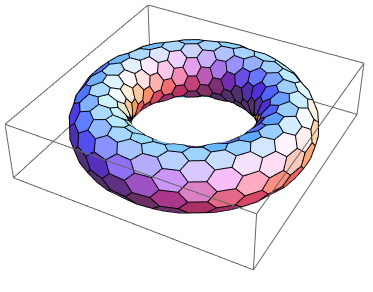
\includegraphics[width=0.75\textwidth]{images/test_image}
	\caption{H-Mode Confinement Time Scaling} ~\\
	\small This plot shows how well the ELMy H-Mode Scaling Law does for fitting $\tau_E$ to the ITER98 database of global tokamaks. For most values, the fit is at least 80\% accurate with the measured value.\cite{tau_iter}
	\label{fig:elmy}
\end{figure}

The energy confinement time -- $\tau_E$ -- is one of the most \replaced{difficult to obtain}{elusive} terms in all of fusion energy. It is an attempt to \replaced{reduce}{boil down} all the \replaced{nonlinear behaviors}{chaotic nature} of plasmas into a simple measure of how fast its internal energy would be ejected from the tokamak if the device was instantaneously shut down. As such, reactor designers have turned toward experimentalists for empirical scalings based on the world's tokamaks (see \cref{fig:elmy}). These all share a form similar to:
\begin{equation}
	\tcboxmath{
	\tau_E = K_\tau \, H \, \frac{
		I_P^{\,\alpha_I} \, R_0^{\,\alpha_R} \, a^{\,\alpha_a} \, \kappa^{\,\alpha_\kappa} \ \overline{n}^{\,\alpha_n} \, B_0^{\,\alpha_B} \, A^{\,\alpha_A}
	}{ P_{src} ^ {\,\alpha_P} }
	}
	\label{eq:tau_gen}
\end{equation}
\myequations{Generalized Confinement Time Scaling Law -- $\tau_E$}
This \replaced{regressional fit}{mouthful of a formula} is how the field actually designs machines (i.e.\ ITER). Let it be known, though, that \replaced{fits of this kind}{these fits} often do remarkable well, having relative errors less than 20\% on interpolated data. The new terms in this equation are: $P_{src}$, $K_\tau$, H, A, and the $\alpha_{\,\square}$ factors.

First, the loss power is a metric used in the engineering community to quantify the power being transported out of the ``core'' of the plasma by charged particles (i.e.\ not the neutrons). \cite{process} To optimize fits, experimentalists have defined this as a combination of the source power terms:
\begin{equation}
	\label{eq:pl}
	P_{src} = P_\alpha + P_H + P_\Omega
\end{equation}
\myequations{Loss Power -- $P_{src}$}
\deleted{However, many have argued that the term should actually be replaced by its correct physics meaning -- the conductive heat loss power. As this model uses the ELMy H-Mode scaling law, which is standard in the field, this alternative definition will not be used:}
%\begin{equation}
%	\tilde P_{src} \approx P_\kappa = P_\alpha + P_H + P_\Omega - P_{BR}
%\end{equation}
Moving on, $K_\tau$ is simply a constant fit-makers use in their scalings. Whereas H is the \replaced{enhancement factor over the empirical fit.}{(H-Mode) scaling factor -- the analogue of $K_\tau$ used by reactor designers. This H factor can be used to artificially boost the confinement of a machine (i.e.\ it adds a little bit of magic).} \replaced{Next,}{Continuing,} A is the average mass number of the fuel source, in atomic mass units. For a 50-50 D-T fuel, this is 2.5, as deuterium weighs two amus and tritium weighs three. Lastly, the alpha factors (e.g.\ $\alpha_n$, $\alpha_a$, $\alpha_P$) are fitting parameters that represent each variable's relative importance in the scaling.

For ELMy H-Mode, this confinement scaling law can be written as:
\begin{equation}
	\tau_E^H = 0.145 \, H \, \frac{
		I_P^{0.93} \, R_0^{1.39} \, a^{0.58} \, \kappa^{0.78} \ \overline{n}^{\, 0.41} \, B_0^{0.15} \, A^{0.19}
	}{ P_{src} ^ {\,0.69} }
	\label{eq:tau_h}
\end{equation}
\myequations{ELMy H-Mode Confinement Time Scaling Law -- $\tau_E^H$}
\replaced{However, similar scaling laws}{Where similar ones} can be \replaced{written}{given} for L-Mode, I-Mode, etc. One final remark to make before moving on is that even these fits have subtleties. The value of $\kappa$, for example, may have a slightly different geometric meaning from tokamak to tokamak. And the exact definition of loss power -- $P_{src}$ -- introduces an even larger area of discrepancy.  \deleted{Although not actually used, a better fit for our model might be one from the author:}
%\begin{equation}
%	\tilde \tau_E = 0.08 \, H \frac{
%		\left( R_0^{1.49} B_0 ^ {0.3} I_P^{0.93} \right) \cdot \left( \epsilon ^ {0.17} A^{0.23}  \kappa ^ {0.56} \right) }{ \tilde P_{src} ^ {\, 0.54} }
%\end{equation}

Returning to the problem at hand, though, this model's Lawson \replaced{Parameter}{Criterion} (eq. \ref{eq:ntaue}) can be simplified after expanding the left-hand side using the Greenwald density and substituting in a confinement time scaling law. \replaced{After a few lines of algebra, this can be transformed}{Albeit a little cumbersome, this can be wrangled} into \replaced{a formula}{an equation} for $B_0$!
\begin{equation}
	\label{eq:b_0_power}
	\tcbhighmath{
	B_0 = \left( \frac{ G_{PB} }{ K_{PB} } \cdot \left( I_P^{\,\alpha_I^*} \, R_0^{ \alpha_R^* } \right)^{-1} \right) ^ { \frac{1}{ \alpha_B } }
	}
\end{equation}
\myequations{Primary Constraint -- $B_0$}
\begin{equation}
	G_{PB} = \frac{ \overline{T} \cdot \left( \, K_P (\sigma v) + K_\Omega  \, \overline{T}^{  \,-3/2 } \, \right) ^ { \alpha_P } }{ \left( \, K_P (\sigma v) + K_\Omega  \, \overline{T}^{  \,-3/2 } - K_{BR} \, \overline{T}^{  \,1/2 } \, \right) }
\end{equation}
\begin{equation}
	K_{PB} = H \cdot \left( \frac{ K_\tau K_n^{\alpha_n^*}}{K_\kappa } \right) \cdot \left(
     \epsilon^{\,\alpha_a} \, \kappa^{\,\alpha_\kappa} \, A^{\,\alpha_A}\right)
\end{equation}

Where we have added new starred alpha values for the density, current, and radius:
\begin{gather}
  \alpha_n^* = 1 + \alpha_n - 2 \alpha_P \\
  \alpha_I^* = \alpha_I + \alpha_n^* \\
  \alpha_R^* = \alpha_R + \alpha_a - 2  \alpha_n^* - 3 \alpha_p
\end{gather}
\deleted{Again, if the alternate definition for heat loss ($\tilde P_{abs}$) were used, another definition for $G_{PB}$ would arise. Quickly reemphasizing, though, these tilded values are not actually used in the model:}
%\begin{equation}
%	\tilde G_{PB} = \frac{ \overline{T} }{ \left( \, K_P (\sigma v) + K_\Omega  \, \overline{T}^{  \,-3/2 } - K_{BR} \, \overline{T}^{  \,1/2 } \, \right) ^ { ( 1 - \alpha_P ) } }
%\end{equation}
This equation for $B_0$ -- derived from power balance -- is thus the primary constraint for reactor designs. It is the first step in connecting the plasma (i.e.\ $\overline n$, $\overline T$, and $I_P$) to its tokamak enclosure (i.e.\ $B_0$ and $R_0$). The remaining step is finding an equation -- or in this case, equations -- for the major radius of the device. These radius equations will collectively be referred to as: the \replaced{limiting constraints.}{Secondary Constraints.}

%\subsection{Exploring the Freidberg Criterion}

\deleted{Before moving onto the Secondary Constraint, it is worth noting that this power balance equation can be written in a triple product form analogous to the Lawson \replaced{Parameter}{Criterion}. For this reason, we will refer to it as the Freidberg Triple Product:}
%\begin{equation}
%	\label{eq:freidberg}
%	R_0^{ \alpha_R^* } \cdot B_0^{\,\alpha_B} \cdot I_P^{\,\alpha_I^*} = \frac{ G_{PB} }{ K_{PB} }
%\end{equation}

%\begin{figure*}[h]
%    \centering
%    \hfill
%    \begin{subfigure}[t]{0.45\textwidth}
%        \centering
%		\begin{adjustbox}{width=\textwidth}
%			\Large
%			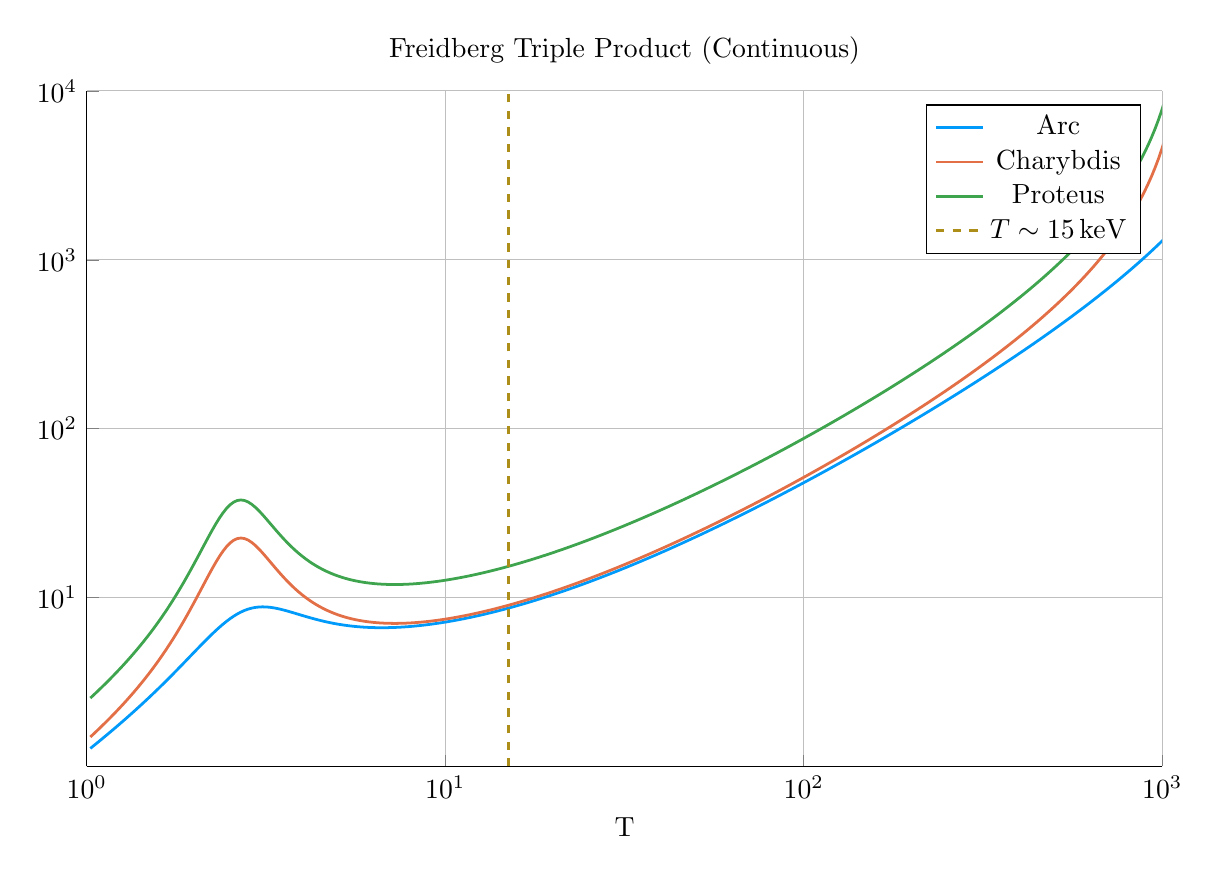
\begin{tikzpicture}[]
\begin{axis}[height = {101.6mm}, ylabel = {}, title = {Freidberg Triple Product (Continuous)}, xmin = {1.0}, xmax = {1000.0}, ymax = {10000.0}, ymode = {log}, xlabel = {T}, {unbounded coords=jump, xticklabel style={rotate = 0}, log basis x=10, xmajorgrids = true, xtick = {1.0,10.0,100.0,1000.0}, xticklabels = {$10^{0}$,$10^{1}$,$10^{2}$,$10^{3}$}, xtick align = inside, axis lines* = left, yticklabel style={rotate = 0}, log basis y=10, ymajorgrids = true, ytick = {10.0,100.0,1000.0,10000.0}, yticklabels = {$10^{1}$,$10^{2}$,$10^{3}$,$10^{4}$}, ytick align = inside, axis lines* = left,     xshift = 0.0mm,
    yshift = 0.0mm,
    axis background/.style={fill={rgb,1:red,1.00000000;green,1.00000000;blue,1.00000000}}
}, xmode = {log}, ymin = {1.001}, width = {152.4mm}]\addplot+ [color = {rgb,1:red,0.00000000;green,0.60560316;blue,0.97868012},
draw opacity=1.0,
line width=1,
solid,mark = none,
mark size = 2.0,
mark options = {
    color = {rgb,1:red,0.00000000;green,0.00000000;blue,0.00000000}, draw opacity = 1.0,
    fill = {rgb,1:red,0.00000000;green,0.60560316;blue,0.97868012}, fill opacity = 1.0,
    line width = 1,
    rotate = 0,
    solid
}]coordinates {
(1.023292992280754, 1.2793221218652944)
(1.0471285480508996, 1.3309195883591072)
(1.0715193052376064, 1.3850036910515204)
(1.096478196143185, 1.4417288746419747)
(1.1220184543019633, 1.5012617022690462)
(1.1481536214968828, 1.5637819142077942)
(1.1748975549395295, 1.6294835657026674)
(1.202264434617413, 1.698576242531264)
(1.2302687708123816, 1.7712863496330842)
(1.2589254117941673, 1.8478584635873476)
(1.288249551693134, 1.928556733480841)
(1.318256738556407, 2.0136663062561424)
(1.3489628825916535, 2.103494741323413)
(1.3803842646028848, 2.1983733642456036)
(1.4125375446227544, 2.2986584896716016)
(1.4454397707459274, 2.4047324181909375)
(1.4791083881682074, 2.5170040789980095)
(1.5135612484362082, 2.635909148564986)
(1.5488166189124815, 2.7619094231676584)
(1.5848931924611136, 2.8954911583354357)
(1.62181009735893, 3.0371620095937497)
(1.6595869074375607, 3.1874461154129454)
(1.6982436524617444, 3.3468767556900265)
(1.7378008287493754, 3.515985900410607)
(1.7782794100389228, 3.6952898405140475)
(1.8197008586099834, 3.8852699797335295)
(1.8620871366628675, 4.08634778460181)
(1.9054607179632472, 4.298852874384422)
(1.9498445997580451, 4.5229833332653655)
(1.9952623149688795, 4.758757610889229)
(2.041737944669529, 5.005957927860106)
(2.0892961308540396, 5.264066012456858)
(2.137962089502232, 5.532193347327445)
(2.1877616239495525, 5.809009942726736)
(2.2387211385683394, 6.092677927494796)
(2.290867652767773, 6.380798757486339)
(2.344228815319922, 6.670385163416938)
(2.3988329190194904, 6.957870427901035)
(2.4547089156850306, 7.239167326284057)
(2.51188643150958, 7.509786194163538)
(2.5703957827688635, 7.7650155007458315)
(2.6302679918953817, 8.000159131951143)
(2.6915348039269156, 8.210813513493981)
(2.7542287033381663, 8.393157056383407)
(2.8183829312644537, 8.544217197329235)
(2.884031503126606, 8.662079281751163)
(2.9512092266663856, 8.746008028642427)
(3.019951720402016, 8.796465438819597)
(3.0902954325135905, 8.815025707881876)
(3.1622776601683795, 8.80420376037562)
(3.2359365692962827, 8.767225560018067)
(3.311311214825911, 8.707773161635059)
(3.3884415613920256, 8.629735524841195)
(3.4673685045253166, 8.536989174977906)
(3.548133892335755, 8.433223490199008)
(3.630780547701014, 8.32181619294888)
(3.715352290971725, 8.205757228033434)
(3.8018939632056115, 8.087614356783817)
(3.890451449942806, 7.9695314352280215)
(3.9810717055349722, 7.853249952422453)
(4.073802778041127, 7.740145297390103)
(4.168693834703354, 7.631270787751151)
(4.265795188015927, 7.527404208691776)
(4.36515832240166, 7.429093260768431)
(4.466835921509632, 7.33669764878841)
(4.570881896148751, 7.250426597707905)
(4.677351412871983, 7.170371324123017)
(4.786300923226384, 7.096532487933503)
(4.897788193684462, 7.028842950140937)
(5.011872336272722, 6.967186322975986)
(5.1286138399136485, 6.911411862292244)
(5.248074602497725, 6.861346254119733)
(5.370317963702527, 6.816802812809654)
(5.495408738576246, 6.777588554906853)
(5.623413251903491, 6.743509552318662)
(5.7543993733715695, 6.714374907663976)
(5.88843655355589, 6.689999637968835)
(6.025595860743578, 6.670206702159046)
(6.165950018614822, 6.654828363817934)
(6.309573444801933, 6.643707043377312)
(6.456542290346556, 6.636695782809513)
(6.606934480075959, 6.633658420300284)
(6.760829753919817, 6.634469551553204)
(6.918309709189364, 6.63901433757021)
(7.079457843841379, 6.6471882052930455)
(7.244359600749901, 6.658896476780433)
(7.413102413009175, 6.674053954122599)
(7.5857757502918375, 6.692584480627425)
(7.762471166286917, 6.714420493592822)
(7.943282347242816, 6.7395025799146895)
(8.128305161640993, 6.767779042630784)
(8.31763771102671, 6.79920548407566)
(8.511380382023766, 6.833744409466334)
(8.709635899560805, 6.871364853329812)
(8.912509381337454, 6.9120420301239145)
(9.120108393559097, 6.955757009615049)
(9.33254300796991, 7.002496416999287)
(9.549925860214358, 7.0522521573385)
(9.772372209558107, 7.105021163593507)
(10.0, 7.160805167339729)
(10.232929922807541, 7.2196104911458425)
(10.471285480508996, 7.281447861469827)
(10.715193052376065, 7.346332241007961)
(10.964781961431852, 7.41428267931583)
(11.220184543019636, 7.485322180621463)
(11.481536214968829, 7.559477587761894)
(11.748975549395297, 7.6367794812276)
(12.02264434617413, 7.7172620923547175)
(12.302687708123818, 7.800963229763945)
(12.589254117941675, 7.887924218206006)
(12.882495516931343, 7.978189849034269)
(13.182567385564074, 8.071808341585202)
(13.489628825916533, 8.168831314805496)
(13.803842646028846, 8.26931376852079)
(14.12537544622754, 8.373314073794269)
(14.454397707459272, 8.480893971874206)
(14.791083881682072, 8.592118581277306)
(15.13561248436208, 8.707056412599798)
(15.488166189124811, 8.825779390690416)
(15.848931924611133, 8.948362883858978)
(16.218100973589298, 9.074885739831279)
(16.595869074375607, 9.205430328195467)
(16.982436524617444, 9.340082589117413)
(17.378008287493753, 9.478932088132577)
(17.78279410038923, 9.622072076850081)
(18.197008586099834, 9.769599559430906)
(18.620871366628677, 9.921615364726758)
(19.054607179632473, 10.07822422398916)
(19.498445997580454, 10.239534854079999)
(19.952623149688797, 10.405660046135063)
(20.417379446695296, 10.576716759651381)
(20.892961308540396, 10.752826221987263)
(21.379620895022324, 10.9341140332813)
(21.87761623949553, 11.120710276812883)
(22.3872113856834, 11.312749634842634)
(22.908676527677734, 11.510371509986186)
(23.442288153199225, 11.7137201521892)
(23.9883291901949, 11.922944791385861)
(24.547089156850298, 12.138199775936432)
(25.118864315095795, 12.359644716953252)
(25.703957827688633, 12.587444638637452)
(26.302679918953814, 12.821770134761826)
(26.915348039269155, 13.062797531448128)
(27.542287033381662, 13.310709056400045)
(28.183829312644534, 13.565693014765834)
(28.84031503126606, 13.82794397181769)
(29.512092266663856, 14.097662942647972)
(30.19951720402016, 14.375057589095706)
(30.902954325135905, 14.660342424130278)
(31.622776601683793, 14.953739023932986)
(32.359365692962825, 15.25547624793148)
(33.11311214825911, 15.565790467056377)
(33.884415613920254, 15.884925800504542)
(34.673685045253166, 16.213134361308995)
(35.48133892335755, 16.550676511031238)
(36.30780547701014, 16.8978211239089)
(37.15352290971726, 17.254845860808384)
(38.018939632056124, 17.622037453350618)
(38.90451449942807, 17.999691998596774)
(39.810717055349734, 18.38811526470027)
(40.73802778041128, 18.78762300795229)
(41.68693834703355, 19.198541301669295)
(42.65795188015925, 19.6212068773937)
(43.65158322401658, 20.05596748532388)
(44.6683592150963, 20.503182229545445)
(45.708818961487495, 20.963222013454047)
(46.77351412871981, 21.436469871175646)
(47.86300923226383, 21.923321410447826)
(48.97788193684461, 22.424185232528163)
(50.11872336272722, 22.939483374951877)
(51.28613839913648, 23.469651771317768)
(52.48074602497726, 24.015140728856327)
(53.70317963702527, 24.576415424552575)
(54.954087385762456, 25.153956420636177)
(56.23413251903491, 25.748260200293693)
(57.543993733715695, 26.35983972450207)
(58.8843655355589, 26.989225010929704)
(60.25595860743578, 27.636963735901347)
(61.65950018614822, 28.303621860475566)
(63.09573444801933, 28.989784281739404)
(64.56542290346556, 29.69605551048393)
(66.06934480075961, 30.423060376486795)
(67.60829753919819, 31.171444762694403)
(69.18309709189366, 31.941876369666343)
(70.79457843841381, 32.735045511719214)
(72.44359600749902, 33.55166594628614)
(74.13102413009177, 34.39247573809195)
(75.85775750291836, 35.25823815983267)
(77.62471166286916, 36.14974263114321)
(79.43282347242814, 37.06780569773617)
(81.2830516164099, 38.013272052702476)
(83.17637711026708, 38.98701560207701)
(85.11380382023764, 39.989940581159736)
(87.09635899560806, 41.02298269407601)
(89.12509381337455, 42.08711036866879)
(91.20108393559097, 43.18332598001413)
(93.3254300796991, 44.312667194688736)
(95.49925860214358, 45.476208349136186)
(97.72372209558107, 46.675061895023376)
(100.0, 47.910379911219174)
(102.32929922807536, 49.1833556845266)
(104.71285480508996, 50.49522536463268)
(107.1519305237606, 51.84726969599379)
(109.64781961431851, 53.24081583131803)
(112.2018454301963, 54.67723923102123)
(114.81536214968828, 56.15796565338645)
(117.48975549395291, 57.684473240449044)
(120.22644346174131, 59.258294704948604)
(123.02687708123811, 60.88101962402365)
(125.89254117941675, 62.55429684569091)
(128.82495516931337, 64.27983701453458)
(131.82567385564073, 66.05941522345191)
(134.89628825916532, 67.89487379874117)
(138.03842646028852, 69.78812522630338)
(141.2537544622754, 71.74115522723595)
(144.5439770745928, 73.75602599165504)
(147.91083881682073, 75.83487958017014)
(151.35612484362088, 77.97994150307832)
(154.88166189124811, 80.19352448802711)
(158.48931924611142, 82.47803244763931)
(162.18100973589299, 84.83596466314262)
(165.95869074375614, 87.2699201708478)
(169.82436524617444, 89.7826024444658)
(173.78008287493762, 92.3768242568097)
(177.82794100389228, 95.05551286856803)
(181.97008586099827, 97.82171548255974)
(186.20871366628674, 100.6786050083681)
(190.54607179632464, 103.62948615355889)
(194.98445997580455, 106.67780186293392)
(199.52623149688787, 109.82714012887666)
(204.17379446695296, 113.08124119760298)
(208.92961308540387, 116.44400519767774)
(213.79620895022325, 119.91950022156021)
(218.77616239495518, 123.51197088641831)
(223.872113856834, 127.2258474138247)
(229.08676527677724, 131.06575526002374)
(234.42288153199226, 135.0365253375378)
(239.88329190194898, 139.14320487005486)
(245.4708915685031, 143.39106892630025)
(251.18864315095797, 147.785632682383)
(257.03957827688646, 152.33266446627786)
(263.02679918953817, 157.03819964265176)
(269.1534803926917, 161.908555401256)
(275.4228703338166, 166.9503465175865)
(281.8382931264455, 172.1705021605638)
(288.40315031266056, 177.57628382861546)
(295.1209226666387, 183.175304502876)
(301.9951720402016, 188.97554911427625)
(309.0295432513592, 194.98539643459995)
(316.22776601683796, 201.21364248106408)
(323.5936569296281, 207.66952561997678)
(331.1311214825911, 214.36275345331575)
(338.84415613920237, 221.30353162896512)
(346.73685045253166, 228.50259481386476)
(354.8133892335753, 235.97123994530904)
(363.0780547701014, 243.7213619906034)
(371.5352290971724, 251.7654924325556)
(380.1893963205613, 260.11684072588844)
(389.04514499428046, 268.78933899522207)
(398.1071705534973, 277.7976902739334)
(407.3802778041126, 287.1574206152656)
(416.8693834703355, 296.88493544311495)
(426.57951880159254, 306.99758055039047)
(436.5158322401661, 317.51370819846284)
(446.683592150963, 328.45274882261293)
(457.0881896148752, 339.83528890503925)
(467.73514128719813, 351.6831556525324)
(478.6300923226385, 364.019509161591)
(489.77881936844614, 376.86894288507557)
(501.18723362727246, 390.25759326505363)
(512.8613839913648, 404.2132595327318)
(524.8074602497728, 418.76553479281586)
(537.0317963702527, 433.94594965392275)
(549.5408738576248, 449.78812983073925)
(562.341325190349, 466.32796933763944)
(575.4399373371566, 483.6038210717674)
(588.843655355589, 501.65670694780766)
(602.5595860743575, 520.5305498494844)
(616.5950018614822, 540.2724301816861)
(630.957344480193, 560.9328700805296)
(645.6542290346556, 582.566148886756)
(660.6934480075957, 605.2306538385934)
(676.0829753919819, 628.989270851766)
(691.8309709189363, 653.90982069593)
(707.945784384138, 680.0655469086195)
(724.4359600749899, 707.5356627471048)
(741.3102413009177, 736.4059656912784)
(758.5775750291835, 766.7695294432701)
(776.247116628692, 798.727485079221)
(794.3282347242813, 832.3899050561196)
(812.8305161640995, 867.8768062379246)
(831.7637711026708, 905.319291075073)
(851.1380382023768, 944.8608496698408)
(870.9635899560806, 986.6588498377013)
(891.2509381337459, 1030.8862476245677)
(912.0108393559096, 1077.7335573068228)
(933.2543007969915, 1127.411128001834)
(954.992586021436, 1180.1517840590136)
(977.2372209558112, 1236.213898917512)
(1000.0, 1295.8849878014776)
(1023.2929922807537, 1359.4859243956064)
(1047.1285480508996, 1427.3759117201514)
(1071.519305237606, 1499.9583694362552)
(1096.4781961431852, 1577.687940957739)
(1122.018454301963, 1661.0788770147035)
(1148.1536214968828, 1750.7151218116257)
(1174.897554939529, 1847.262519332875)
(1202.2644346174131, 1951.4836786284711)
(1230.268770812381, 2064.2561993145287)
(1258.9254117941675, 2186.595178121113)
(1288.2495516931335, 2319.6812176589965)
(1318.2567385564075, 2464.8955729365553)
(1348.9628825916532, 2623.864652612861)
(1380.3842646028852, 2798.516914142382)
(1412.537544622754, 2991.1563761807724)
(1445.439770745928, 3204.5587002127395)
(1479.1083881682073, 3442.098361225498)
(1513.5612484362086, 3707.9193124396793)
(1548.816618912481, 4007.1675479581536)
(1584.893192461114, 4346.313439566653)
(1621.8100973589299, 4733.607058236353)
(1659.5869074375614, 5179.735215473649)
(1698.2436524617442, 5698.792798685391)
(1737.8008287493763, 6309.758994188134)
(1778.2794100389228, 7038.813610830222)
(1819.7008586099826, 7923.109724291594)
(1862.0871366628676, 9017.195901992123)
(1905.4607179632462, 10404.546791614655)
(1949.8445997580454, 12219.667076115855)
(1995.2623149688789, 14694.120959228087)
(2041.7379446695295, 18263.35087394861)
(2089.296130854039, 23854.381911656048)
(2137.9620895022326, 33852.2908799337)
(2187.761623949552, 56824.35846897241)
(2238.72113856834, 164426.65765500255)
(2290.8676527677726, -199130.5391041138)
(2344.228815319923, -63592.36702962983)
(2398.83291901949, -38401.823826757456)
(2454.708915685031, -27793.602877328278)
(2511.88643150958, -21952.016301942476)
(2570.3957827688646, -18256.558428890912)
(2630.2679918953813, -15710.129369983011)
(2691.5348039269165, -13850.495487055317)
(2754.2287033381663, -12434.055966251428)
(2818.382931264455, -11320.247131391827)
(2884.031503126606, -10422.274535612401)
(2951.209226666387, -9683.646906144215)
(3019.9517204020162, -9066.01284792254)
(3090.295432513592, -8542.595957682206)
(3162.2776601683795, -8093.376345071255)
(3235.936569296281, -7704.429898465926)
(3311.311214825911, -7364.644013312067)
(3388.441561392024, -7065.587403461628)
(3467.368504525317, -6800.6560221766695)
(3548.133892335753, -6564.6034987731455)
(3630.780547701014, -6353.209298630934)
(3715.352290971724, -6163.039676144607)
(3801.8939632056126, -5991.272496174683)
(3890.4514499428046, -5835.566864306992)
(3981.0717055349733, -5693.964740791021)
(4073.802778041126, -5564.815743424234)
(4168.693834703355, -5446.719003997193)
(4265.795188015925, -5338.477730561384)
(4365.158322401661, -5239.0633500512895)
(4466.835921509631, -5147.586954620055)
(4570.881896148751, -5063.276373046262)
(4677.351412871981, -4985.457615476961)
(4786.300923226385, -4913.539746969296)
(4897.7881936844615, -4847.002480006052)
(5011.872336272725, -4785.385915699954)
(5128.613839913648, -4728.282033811321)
(5248.074602497728, -4675.327569873742)
(5370.317963702527, -4626.198049926041)
(5495.408738576249, -4580.602740941166)
(5623.413251903491, -4538.280376245746)
(5754.399373371566, -4498.995513494782)
(5888.43655355589, -4462.535419726061)
(6025.595860743575, -4428.7073965916015)
(6165.9500186148225, -4397.336474861534)
(6309.57344480193, -4368.26342005518)
(6456.542290346556, -4341.343001287243)
(6606.934480075957, -4316.442483667796)
(6760.829753919818, -4293.440311248033)
(6918.309709189362, -4272.224953180315)
(7079.457843841381, -4252.693889506939)
(7244.359600749898, -4234.752717844742)
(7413.102413009177, -4218.314364047006)
(7585.775750291836, -4203.29838315304)
(7762.4711662869195, -4189.630338739936)
(7943.282347242814, -4177.241250766746)
(8128.305161640995, -4166.067102901534)
(8317.63771102671, -4156.048402374031)
(8511.380382023768, -4147.1297856871)
(8709.635899560806, -4139.259664786595)
(8912.509381337459, -4132.389908913949)
(9120.108393559096, -4126.475558010264)
(9332.543007969914, -4121.474564078605)
(9549.92586021436, -4117.347557371377)
(9772.372209558112, -4114.057634664823)
(10000.0, -4111.57016722244)
};
\addlegendentry{Arc}
\addplot+ [color = {rgb,1:red,0.88887350;green,0.43564919;blue,0.27812294},
draw opacity=1.0,
line width=1,
solid,mark = none,
mark size = 2.0,
mark options = {
    color = {rgb,1:red,0.00000000;green,0.00000000;blue,0.00000000}, draw opacity = 1.0,
    fill = {rgb,1:red,0.88887350;green,0.43564919;blue,0.27812294}, fill opacity = 1.0,
    line width = 1,
    rotate = 0,
    solid
}]coordinates {
(1.023292992280754, 1.4951205905179736)
(1.0471285480508996, 1.564933213170644)
(1.0715193052376064, 1.6391186292624738)
(1.096478196143185, 1.7180622084543624)
(1.1220184543019633, 1.8021941616786232)
(1.1481536214968828, 1.8919958608612342)
(1.1748975549395295, 1.9880071734245173)
(1.202264434617413, 2.0908349882404913)
(1.2302687708123816, 2.2011631409423815)
(1.2589254117941673, 2.3197639825513616)
(1.288249551693134, 2.4475118764272956)
(1.318256738556407, 2.5853989543987748)
(1.3489628825916535, 2.7345535126429543)
(1.3803842646028848, 2.896261479310555)
(1.4125375446227544, 3.0719914348155988)
(1.4454397707459274, 3.263423704587518)
(1.4791083881682074, 3.472484060035992)
(1.5135612484362082, 3.7013825352091754)
(1.5488166189124815, 3.952657759716108)
(1.5848931924611136, 4.229226968304124)
(1.62181009735893, 4.534441388686033)
(1.6595869074375607, 4.872145900529501)
(1.6982436524617444, 5.2467405015013435)
(1.7378008287493754, 5.663238917158036)
(1.7782794100389228, 6.127316227593624)
(1.8197008586099834, 6.645332071138777)
(1.8620871366628675, 7.224308067533204)
(1.9054607179632472, 7.871826706510841)
(1.9498445997580451, 8.595803300518865)
(1.9952623149688795, 9.404062589508452)
(2.041737944669529, 10.303628945858334)
(2.0892961308540396, 11.29961963663557)
(2.137962089502232, 12.393627534998426)
(2.1877616239495525, 13.581517950512376)
(2.2387211385683394, 14.850682342251654)
(2.290867652767773, 16.177033787448202)
(2.344228815319922, 17.522414780403594)
(2.3988329190194904, 18.833549197849237)
(2.4547089156850306, 20.04397470378986)
(2.51188643150958, 21.08013836114596)
(2.5703957827688635, 21.871665671436986)
(2.6302679918953817, 22.36384995966289)
(2.6915348039269156, 22.528612673585403)
(2.7542287033381663, 22.369948558667186)
(2.8183829312644537, 21.921824163906248)
(2.884031503126606, 21.23964003953929)
(2.9512092266663856, 20.38872623352358)
(3.019951720402016, 19.433663321546106)
(3.0902954325135905, 18.430838621774875)
(3.1622776601683795, 17.424807209897704)
(3.2359365692962827, 16.44773839121447)
(3.311311214825911, 15.520762283244057)
(3.3884415613920256, 14.656147043575608)
(3.4673685045253166, 13.859584188165677)
(3.548133892335755, 13.132200852217746)
(3.630780547701014, 12.47216002027133)
(3.715352290971725, 11.875847565048533)
(3.8018939632056115, 11.33870683093359)
(3.890451449942806, 10.855798600216186)
(3.9810717055349722, 10.42215943225786)
(4.073802778041127, 10.033018273423268)
(4.168693834703354, 9.683916918667496)
(4.265795188015927, 9.370767350264446)
(4.36515832240166, 9.089869055571175)
(4.466835921509632, 8.837902043453784)
(4.570881896148751, 8.6119060006025)
(4.677351412871983, 8.409252359661203)
(4.786300923226384, 8.227613555065604)
(4.897788193684462, 8.064932075325121)
(5.011872336272722, 7.91939082590377)
(5.1286138399136485, 7.789385611127785)
(5.248074602497725, 7.673500098221017)
(5.370317963702527, 7.570483353424563)
(5.495408738576246, 7.479229879408585)
(5.623413251903491, 7.398761994753704)
(5.7543993733715695, 7.328214353551413)
(5.88843655355589, 7.266820388638273)
(6.025595860743578, 7.213900464232118)
(6.165950018614822, 7.168851535440971)
(6.309573444801933, 7.131138128615018)
(6.456542290346556, 7.100284474923121)
(6.606934480075959, 7.075867648120776)
(6.760829753919817, 7.057511575241371)
(6.918309709189364, 7.0448818053617135)
(7.079457843841379, 7.03768093643693)
(7.244359600749901, 7.035644614021524)
(7.413102413009175, 7.0385380224948895)
(7.5857757502918375, 7.046152816528243)
(7.762471166286917, 7.058304415490602)
(7.943282347242816, 7.074829633505994)
(8.128305161640993, 7.095584590601089)
(8.31763771102671, 7.120442873022589)
(8.511380382023766, 7.149293910866733)
(8.709635899560805, 7.182041545986132)
(8.912509381337454, 7.218602766766122)
(9.120108393559097, 7.258906589488317)
(9.33254300796991, 7.30289306863743)
(9.549925860214358, 7.350512420953691)
(9.772372209558107, 7.401724249797036)
(10.0, 7.456496858332535)
(10.232929922807541, 7.514806641813107)
(10.471285480508996, 7.576637547200618)
(10.715193052376065, 7.641980601233738)
(10.964781961431852, 7.710833485482428)
(11.220184543019636, 7.7832001671752655)
(11.481536214968829, 7.859090571781095)
(11.748975549395297, 7.93852029572274)
(12.02264434617413, 8.02151035478933)
(12.302687708123818, 8.108086964714632)
(12.589254117941675, 8.198281350809156)
(12.882495516931343, 8.292129583902065)
(13.182567385564074, 8.38967244017214)
(13.489628825916533, 8.490955282751791)
(13.803842646028846, 8.596027963097924)
(14.12537544622754, 8.704944740753675)
(14.454397707459272, 8.817764219656572)
(14.791083881682072, 8.934549299966482)
(15.13561248436208, 9.055367144163561)
(15.488166189124811, 9.180289156424717)
(15.848931924611133, 9.309390974391308)
(16.218100973589298, 9.442752472549282)
(16.595869074375607, 9.580457776539694)
(16.982436524617444, 9.722595287804594)
(17.378008287493753, 9.869257717974659)
(17.78279410038923, 10.020542133007641)
(18.197008586099834, 10.176550005569382)
(18.620871366628677, 10.337387276815504)
(19.054607179632473, 10.50316442620314)
(19.498445997580454, 10.673996549542666)
(19.952623149688797, 10.850003445038157)
(20.417379446695296, 11.031309707177495)
(20.892961308540396, 11.21804482837071)
(21.379620895022324, 11.410343308360655)
(21.87761623949553, 11.608344770822882)
(22.3872113856834, 11.81219408853973)
(22.908676527677734, 12.02204151524775)
(23.442288153199225, 12.238042826008586)
(23.9883291901949, 12.460359464612567)
(24.547089156850298, 12.689158699600375)
(25.118864315095795, 12.924613787966877)
(25.703957827688633, 13.166904147140388)
(26.302679918953814, 13.41621553534255)
(26.915348039269155, 13.672740240532336)
(27.542287033381662, 13.936677278161076)
(28.183829312644534, 14.208232597989184)
(28.84031503126606, 14.487619300239052)
(29.512092266663856, 14.775057861382548)
(30.19951720402016, 15.070776369886339)
(30.902954325135905, 15.37501077226307)
(31.622776601683793, 15.688005129802471)
(32.359365692962825, 16.010011886382863)
(33.11311214825911, 16.341292147791066)
(33.884415613920254, 16.68211597300732)
(34.673685045253166, 17.03276267794145)
(35.48133892335755, 17.39352115213756)
(36.30780547701014, 17.764690188997083)
(37.15352290971726, 18.146578830103802)
(38.018939632056124, 18.539506724270478)
(38.90451449942807, 18.943804501964173)
(39.810717055349734, 19.35981416580702)
(40.73802778041128, 19.78788949789105)
(41.68693834703355, 20.228396484690027)
(42.65795188015925, 20.681713760397738)
(43.65158322401658, 21.14823306957214)
(44.6683592150963, 21.628359750016873)
(45.708818961487495, 22.122513236887862)
(46.77351412871981, 22.631127589071507)
(47.86300923226383, 23.154652038944235)
(48.97788193684461, 23.693551566689866)
(50.11872336272722, 24.248307500422708)
(51.28613839913648, 24.81941814344006)
(52.48074602497726, 25.40739943000132)
(53.70317963702527, 26.012785611181393)
(54.954087385762456, 26.636129972209588)
(56.23413251903491, 27.278005583239572)
(57.543993733715695, 27.939006085113782)
(58.8843655355589, 28.619746512118212)
(60.25595860743578, 29.320864153728113)
(61.65950018614822, 30.043019457491077)
(63.09573444801933, 30.78689697533123)
(64.56542290346556, 31.553206355705683)
(66.06934480075961, 32.342683384201756)
(67.60829753919819, 33.1560910753331)
(69.18309709189366, 33.99422081847368)
(70.79457843841381, 34.85789358106391)
(72.44359600749902, 35.74796117243211)
(74.13102413009177, 36.66530757179922)
(75.85775750291836, 37.61085032427685)
(77.62471166286916, 38.585542008928385)
(79.43282347242814, 39.590371782110765)
(81.2830516164099, 40.626367008673384)
(83.17637711026708, 41.6945949622166)
(85.11380382023764, 42.79616463935998)
(87.09635899560806, 43.93222865410277)
(89.12509381337455, 45.10398524216428)
(91.20108393559097, 46.312680373935066)
(93.3254300796991, 47.55960998420363)
(95.49925860214358, 48.846122326207784)
(97.72372209558107, 50.173620458119096)
(100.0, 51.54356487067436)
(102.32929922807536, 52.95747626532544)
(104.71285480508996, 54.41693849299136)
(107.1519305237606, 55.923601664269995)
(109.64781961431851, 57.47918544280937)
(112.2018454301963, 59.08548253445107)
(114.81536214968828, 60.7443623857563)
(117.48975549395291, 62.457775106607066)
(120.22644346174131, 64.22775563276005)
(123.02687708123811, 66.056428145572)
(125.89254117941675, 67.94601076717356)
(128.82495516931337, 69.89882055189202)
(131.82567385564073, 71.91727879488154)
(134.89628825916532, 74.00391668218201)
(138.03842646028852, 76.16138130766076)
(141.2537544622754, 78.3924420847494)
(144.5439770745928, 80.69999758329622)
(147.91083881682073, 83.08708282452531)
(151.35612484362088, 85.55687707004566)
(154.88166189124811, 88.11271214409096)
(158.48931924611142, 90.75808133175465)
(162.18100973589299, 93.49664889992715)
(165.95869074375614, 96.33226029201289)
(169.82436524617444, 99.26895305232473)
(173.78008287493762, 102.31096853994755)
(177.82794100389228, 105.46276450947596)
(181.97008586099827, 108.72902860170117)
(186.20871366628674, 112.11469287647785)
(190.54607179632464, 115.62494942584757)
(194.98445997580455, 119.26526719641967)
(199.52623149688787, 123.04141011921602)
(204.17379446695296, 126.95945666821108)
(208.92961308540387, 131.02582097999962)
(213.79620895022325, 135.2472756812402)
(218.77616239495518, 139.63097658645023)
(223.872113856834, 144.18448944666136)
(229.08676527677724, 148.91581894960441)
(234.42288153199226, 153.83344019485565)
(239.88329190194898, 158.94633289305446)
(245.4708915685031, 164.26401856738593)
(251.18864315095797, 169.79660106845054)
(257.03957827688646, 175.55481075105723)
(263.02679918953817, 181.55005270400406)
(269.1534803926917, 187.7944594723955)
(275.4228703338166, 194.30094876737874)
(281.8382931264455, 201.0832867215087)
(288.40315031266056, 208.15615732051404)
(295.1209226666387, 215.53523872603785)
(301.9951720402016, 223.237287297158)
(309.0295432513592, 231.2802302371631)
(316.22776601683796, 239.68326790746542)
(323.5936569296281, 248.4669870112523)
(331.1311214825911, 257.65348601497806)
(338.84415613920237, 267.2665143791625)
(346.73685045253166, 277.33162740455674)
(354.8133892335753, 287.8763587728208)
(363.0780547701014, 298.93041319838267)
(371.5352290971724, 310.52588194744516)
(380.1893963205613, 322.69748449781565)
(389.04514499428046, 335.4828400810511)
(398.1071705534973, 348.9227735266097)
(407.3802778041126, 363.06166054010185)
(416.8693834703355, 377.9478185529364)
(426.57951880159254, 393.63395021579794)
(436.5158322401661, 410.17764807782527)
(446.683592150963, 427.6419704997236)
(457.0881896148752, 446.09610082021544)
(467.73514128719813, 465.61610416467147)
(478.6300923226385, 486.2857991992019)
(489.77881936844614, 508.1977657291999)
(501.18723362727246, 531.4545135001769)
(512.8613839913648, 556.1698431170108)
(524.8074602497728, 582.4704369653913)
(537.0317963702527, 610.4977268045958)
(549.5408738576248, 640.4100958466778)
(562.341325190349, 672.3854873698006)
(575.4399373371566, 706.6245102131318)
(588.843655355589, 743.3541552006656)
(602.5595860743575, 782.8322674726481)
(616.5950018614822, 825.3529604033479)
(630.957344480193, 871.253210805378)
(645.6542290346556, 920.9209474913584)
(660.6934480075957, 974.8050431796295)
(676.0829753919819, 1033.4277536202915)
(691.8309709189363, 1097.4003329905518)
(707.945784384138, 1167.442813860071)
(724.4359600749899, 1244.409307817316)
(741.3102413009177, 1329.3207121308826)
(758.5775750291835, 1423.4074814235566)
(776.247116628692, 1528.1662733492376)
(794.3282347242813, 1645.4360188093654)
(812.8305161640995, 1777.5016588970052)
(831.7637711026708, 1927.2380456000428)
(851.1380382023768, 2098.313399614084)
(870.9635899560806, 2295.4832135411857)
(891.2509381337459, 2525.0252615139284)
(912.0108393559096, 2795.401629083202)
(933.2543007969915, 3118.2991515065182)
(954.992586021436, 3510.327175414144)
(977.2372209558112, 3995.9141566747626)
(1000.0, 4612.522449068273)
(1023.2929922807537, 5420.678931670947)
(1047.1285480508996, 6524.954016908558)
(1071.519305237606, 8122.931037204398)
(1096.4781961431852, 10638.194039946591)
(1122.018454301963, 15172.86374695544)
(1148.1536214968828, 25773.848015735388)
(1174.897554939529, 79055.66874518472)
(1202.2644346174131, -79563.49335752385)
(1230.268770812381, -27114.50369707553)
(1258.9254117941675, -16580.394253178674)
(1288.2495516931335, -12064.46874388598)
(1318.2567385564075, -9557.280170214326)
(1348.9628825916532, -7963.778441976489)
(1380.3842646028852, -6862.484637048789)
(1412.537544622754, -6056.620287707458)
(1445.439770745928, -5441.976541218205)
(1479.1083881682073, -4958.208444307301)
(1513.5612484362086, -4567.953239706093)
(1548.816618912481, -4246.840667527393)
(1584.893192461114, -3978.2971894125826)
(1621.8100973589299, -3750.6589387396657)
(1659.5869074375614, -3555.4790834249948)
(1698.2436524617442, -3386.4902442467055)
(1737.8008287493763, -3238.944190744883)
(1778.2794100389228, -3109.1778587358845)
(1819.7008586099826, -2994.3201078635752)
(1862.0871366628676, -2892.088692141341)
(1905.4607179632462, -2800.6466452068157)
(1949.8445997580454, -2718.4987386244966)
(1995.2623149688789, -2644.4155477053305)
(2041.7379446695295, -2577.376902340934)
(2089.296130854039, -2516.5291850771846)
(2137.9620895022326, -2461.1526753580274)
(2187.761623949552, -2410.6362869243053)
(2238.72113856834, -2364.457816397218)
(2290.8676527677726, -2322.168349671393)
(2344.228815319923, -2283.3798396019106)
(2398.83291901949, -2247.7551272193396)
(2454.708915685031, -2214.9998635185793)
(2511.88643150958, -2184.8559225055)
(2570.3957827688646, -2157.0959939235945)
(2630.2679918953813, -2131.519116326531)
(2691.5348039269165, -2107.946965092251)
(2754.2287033381663, -2086.220750607544)
(2818.382931264455, -2066.1986127338305)
(2884.031503126606, -2047.753421328358)
(2951.209226666387, -2030.7709108670972)
(3019.9517204020162, -2015.1480914275285)
(3090.295432513592, -2000.7918894196343)
(3162.2776601683795, -1987.6179802266126)
(3235.936569296281, -1975.5497818751294)
(3311.311214825911, -1964.5175844059183)
(3388.441561392024, -1954.4577939192473)
(3467.368504525317, -1945.3122748929197)
(3548.133892335753, -1937.0277742317169)
(3630.780547701014, -1929.5554180616418)
(3715.352290971724, -1922.850268032745)
(3801.8939632056126, -1916.870932190606)
(3890.4514499428046, -1911.57921953293)
(3981.0717055349733, -1906.9398348640711)
(4073.802778041126, -1902.9201077295872)
(4168.693834703355, -1899.4897512055145)
(4265.795188015925, -1896.620646776375)
(4365.158322401661, -1894.2866520690857)
(4466.835921509631, -1892.4634286597154)
(4570.881896148751, -1891.1282875505613)
(4677.351412871981, -1890.2600502380594)
(4786.300923226385, -1889.8389235669722)
(4897.7881936844615, -1889.846386801031)
(5011.872336272725, -1890.2650895411505)
(5128.613839913648, -1891.0787592914467)
(5248.074602497728, -1892.2721176452642)
(5370.317963702527, -1893.8308041200567)
(5495.408738576249, -1895.741306900434)
(5623.413251903491, -1897.9908997242362)
(5754.399373371566, -1900.5675843022898)
(5888.43655355589, -1903.460037710858)
(6025.595860743575, -1906.6575642625187)
(6165.9500186148225, -1910.1500514165457)
(6309.57344480193, -1913.9279293382913)
(6456.542290346556, -1917.9821337596147)
(6606.934480075957, -1922.3040718297905)
(6760.829753919818, -1926.8855906584417)
(6918.309709189362, -1931.7189484223481)
(7079.457843841381, -1936.7967875228326)
(7244.359600749898, -1942.1121099667994)
(7413.102413009177, -1947.6582545216322)
(7585.775750291836, -1953.4288755858809)
(7762.4711662869195, -1959.4179236128427)
(7943.282347242814, -1965.6196269995667)
(8128.305161640995, -1972.0284750546755)
(8317.63771102671, -1978.6392026046185)
(8511.380382023768, -1985.4467752535925)
(8709.635899560806, -1992.4463758696804)
(8912.509381337459, -1999.6333919540482)
(9120.108393559096, -2007.003403863219)
(9332.543007969914, -2014.5521738176642)
(9549.92586021436, -2022.275635635897)
(9772.372209558112, -2030.1698851385363)
(10000.0, -2038.2311711716875)
};
\addlegendentry{Charybdis}
\addplot+ [color = {rgb,1:red,0.24222430;green,0.64327509;blue,0.30444865},
draw opacity=1.0,
line width=1,
solid,mark = none,
mark size = 2.0,
mark options = {
    color = {rgb,1:red,0.00000000;green,0.00000000;blue,0.00000000}, draw opacity = 1.0,
    fill = {rgb,1:red,0.24222430;green,0.64327509;blue,0.30444865}, fill opacity = 1.0,
    line width = 1,
    rotate = 0,
    solid
}]coordinates {
(1.023292992280754, 2.541607794182799)
(1.0471285480508996, 2.660269439262049)
(1.0715193052376064, 2.786360666052945)
(1.096478196143185, 2.9205356854657296)
(1.1220184543019633, 3.063524724400726)
(1.1481536214968828, 3.216144715811088)
(1.1748975549395295, 3.3793116995653536)
(1.202264434617413, 3.5540552303333866)
(1.2302687708123816, 3.7415351405622417)
(1.2589254117941673, 3.943061066225367)
(1.288249551693134, 4.160115210605459)
(1.318256738556407, 4.394378896373295)
(1.3489628825916535, 4.647763536834513)
(1.3803842646028848, 4.922446739440267)
(1.4125375446227544, 5.220914330915469)
(1.4454397707459274, 5.546009150273053)
(1.4791083881682074, 5.900987470964557)
(1.5135612484362082, 6.289583849408761)
(1.5488166189124815, 6.716084994646623)
(1.5848931924611136, 7.185412819004359)
(1.62181009735893, 7.703216016525367)
(1.6595869074375607, 8.275968101385919)
(1.6982436524617444, 8.911067487071362)
(1.7378008287493754, 9.616931405348344)
(1.7782794100389228, 10.403069547350476)
(1.8197008586099834, 11.28011429330212)
(1.8620871366628675, 12.25977105091236)
(1.9054607179632472, 13.35463315762688)
(1.9498445997580451, 14.577779867897343)
(1.9952623149688795, 15.942043199129527)
(2.041737944669529, 17.458793128762032)
(2.0892961308540396, 19.136060977302172)
(2.137962089502232, 20.975820417452365)
(2.1877616239495525, 22.970315960561763)
(2.2387211385683394, 25.097532595958718)
(2.290867652767773, 27.316306602413356)
(2.344228815319922, 29.56221049019534)
(2.3988329190194904, 31.74608116935286)
(2.4547089156850306, 33.75751095725075)
(2.51188643150958, 35.47514052683947)
(2.5703957827688635, 36.783633019278696)
(2.6302679918953817, 37.59403412846895)
(2.6915348039269156, 37.861409213680616)
(2.7542287033381663, 37.59339338690544)
(2.8183829312644537, 36.84651350419666)
(2.884031503126606, 35.71217607737041)
(2.9512092266663856, 34.297938025238906)
(3.019951720402016, 32.7101474333056)
(3.0902954325135905, 31.041816586660673)
(3.1622776601683795, 29.366648033881443)
(3.2359365692962827, 27.738068701136157)
(3.311311214825911, 26.191370044328774)
(3.3884415613920256, 24.74722683476745)
(3.4673685045253166, 23.415418019053714)
(3.548133892335755, 22.198121549345238)
(3.630780547701014, 21.09254798062826)
(3.715352290971725, 20.092903807422037)
(3.8018939632056115, 19.19177893589775)
(3.890451449942806, 18.38108281851224)
(3.9810717055349722, 17.65264744406442)
(4.073802778041127, 16.99859494844685)
(4.168693834703354, 16.411544710422163)
(4.265795188015927, 15.884714471437004)
(4.36515832240166, 15.41195382389336)
(4.466835921509632, 14.98773628869399)
(4.570881896148751, 14.607127487360424)
(4.677351412871983, 14.265740825469246)
(4.786300923226384, 13.95968794288132)
(4.897788193684462, 13.685528393702176)
(5.011872336272722, 13.44022117639095)
(5.1286138399136485, 13.221079539988146)
(5.248074602497725, 13.025729733892353)
(5.370317963702527, 12.852073899602395)
(5.495408738576246, 12.698257023730783)
(5.623413251903491, 12.56263771532527)
(5.7543993733715695, 12.443762492389391)
(5.88843655355589, 12.340343232922633)
(6.025595860743578, 12.251237445471617)
(6.165950018614822, 12.175431030586726)
(6.309573444801933, 12.112023229735994)
(6.456542290346556, 12.060213487153016)
(6.606934480075959, 12.01928997975262)
(6.760829753919817, 11.988619598872175)
(6.918309709189364, 11.967639194230097)
(7.079457843841379, 11.955847914691219)
(7.244359600749901, 11.952800503084328)
(7.413102413009175, 11.958101413208741)
(7.5857757502918375, 11.9713996626805)
(7.762471166286917, 11.992384292324001)
(7.943282347242816, 12.020780387385628)
(8.128305161640993, 12.05634556925513)
(8.31763771102671, 12.098866904590224)
(8.511380382023766, 12.14815817865815)
(8.709635899560805, 12.204057487742425)
(8.912509381337454, 12.266425111494739)
(9.120108393559097, 12.33514163131487)
(9.33254300796991, 12.410106265235525)
(9.549925860214358, 12.491235393872094)
(9.772372209558107, 12.578461254933405)
(10.0, 12.67173078704092)
(10.232929922807541, 12.771004606563274)
(10.471285480508996, 12.876256097680587)
(10.715193052376065, 12.98747061772595)
(10.964781961431852, 13.104644781481575)
(11.220184543019636, 13.227785839476955)
(11.481536214968829, 13.356911126572342)
(11.748975549395297, 13.492047578158168)
(12.02264434617413, 13.63323130651227)
(12.302687708123818, 13.780507231376948)
(12.589254117941675, 13.933928759523079)
(12.882495516931343, 14.09355750868674)
(13.182567385564074, 14.259463071806497)
(13.489628825916533, 14.431722818001726)
(13.803842646028846, 14.61042172691412)
(14.12537544622754, 14.795652254101604)
(14.454397707459272, 14.987514224373918)
(14.791083881682072, 15.186114751346102)
(15.13561248436208, 15.391568181104251)
(15.488166189124811, 15.603996058314415)
(15.848931924611133, 15.823527113280903)
(16.218100973589298, 16.050297268642687)
(16.595869074375607, 16.28444966455967)
(16.982436524617444, 16.52613470138716)
(17.378008287493753, 16.77551009883809)
(17.78279410038923, 17.032740971655993)
(18.197008586099834, 17.29799991924191)
(18.620871366628677, 17.571467131209467)
(19.054607179632473, 17.853330506543866)
(19.498445997580454, 18.143785786726287)
(19.952623149688797, 18.443036702400743)
(20.417379446695296, 18.751295133350837)
(20.892961308540396, 19.068781281617248)
(21.379620895022324, 19.395723857799993)
(21.87761623949553, 19.732360279556918)
(22.3872113856834, 20.07893688465498)
(22.908676527677734, 20.435709155345496)
(23.442288153199225, 20.80294195721)
(23.9883291901949, 21.18090978994461)
(24.547089156850298, 21.56989705277924)
(25.118864315095795, 21.970198322942146)
(25.703957827688633, 22.38211864817966)
(26.302679918953814, 22.80597385351111)
(26.915348039269155, 23.242090862565636)
(27.542287033381662, 23.69080803388798)
(28.183829312644534, 24.152475512639914)
(28.84031503126606, 24.627455598164808)
(29.512092266663856, 25.116123127923363)
(30.19951720402016, 25.618865878350537)
(30.902954325135905, 26.136084983226056)
(31.622776601683793, 26.66819537019469)
(32.359365692962825, 27.21562621611788)
(33.11311214825911, 27.778821421984443)
(33.884415613920254, 28.358240108157208)
(34.673685045253166, 28.954357130782476)
(35.48133892335755, 29.567663620241944)
(36.30780547701014, 30.19866754258214)
(37.15352290971726, 30.847894284913846)
(38.018939632056124, 31.51588726583507)
(38.90451449942807, 32.20320857199487)
(39.810717055349734, 32.91043962198263)
(40.73802778041128, 33.63818185879886)
(41.68693834703355, 34.3870574722384)
(42.65795188015925, 35.15771015259646)
(43.65158322401658, 35.95080587719262)
(44.6683592150963, 36.76703373129632)
(45.708818961487495, 37.60710676513331)
(46.77351412871981, 38.4717628887521)
(47.86300923226383, 39.36176580663712)
(48.97788193684461, 40.27790599406875)
(50.11872336272722, 41.221001717351704)
(51.28613839913648, 42.191900100162)
(52.48074602497726, 43.191478238388044)
(53.70317963702527, 44.22064436609695)
(54.954087385762456, 45.280339075024756)
(56.23413251903491, 46.371536590898835)
(57.543993733715695, 47.495246109249514)
(58.8843655355589, 48.652513194104685)
(60.25595860743578, 49.84442124296793)
(61.65950018614822, 51.072093021729245)
(63.09573444801933, 52.33669227339113)
(64.56542290346556, 53.63942540474236)
(66.06934480075961, 54.98154325538067)
(67.60829753919819, 56.36434295377245)
(69.18309709189366, 57.789169865346466)
(70.79457843841381, 59.25741963794928)
(72.44359600749902, 60.77054035034607)
(74.13102413009177, 62.33003476983249)
(75.85775750291836, 63.937462725434315)
(77.62471166286916, 65.59444360361373)
(79.43282347242814, 67.30265897195221)
(81.2830516164099, 69.0638553521895)
(83.17637711026708, 70.87984711066403)
(85.11380382023764, 72.75251954256814)
(87.09635899560806, 74.68383209236042)
(89.12509381337455, 76.67582176114273)
(91.20108393559097, 78.7306066986749)
(93.3254300796991, 80.85038999390731)
(95.49925860214358, 83.03746367686449)
(97.72372209558107, 85.29421294566431)
(100.0, 87.62312063348622)
(102.32929922807536, 90.02677193142016)
(104.71285480508996, 92.50785938433819)
(107.1519305237606, 95.06918817824645)
(109.64781961431851, 97.71368173900832)
(112.2018454301963, 100.44438766387783)
(114.81536214968828, 103.26448400898384)
(117.48975549395291, 106.17728595774017)
(120.22644346174131, 109.18625289717419)
(123.02687708123811, 112.29499593144574)
(125.89254117941675, 115.50728586362742)
(128.82495516931337, 118.82706168110607)
(131.82567385564073, 122.25843958023576)
(134.89628825916532, 125.80572257141799)
(138.03842646028852, 129.4734107078804)
(141.2537544622754, 133.26621198560582)
(144.5439770745928, 137.18905396595565)
(147.91083881682073, 141.2470961770721)
(151.35612484362088, 145.4457433551635)
(154.88166189124811, 149.7906595922786)
(158.48931924611142, 154.28778346327053)
(162.18100973589299, 158.94334421135093)
(165.95869074375614, 163.76387907906673)
(169.82436524617444, 168.75625187972454)
(173.78008287493762, 173.92767291090885)
(177.82794100389228, 179.2857203416813)
(181.97008586099827, 184.8383631466899)
(186.20871366628674, 190.5939858119774)
(190.54607179632464, 196.56141487722155)
(194.98445997580455, 202.74994753370547)
(199.52623149688787, 209.16938244496987)
(204.17379446695296, 215.8300529962404)
(208.92961308540387, 222.74286319776243)
(213.79620895022325, 229.91932649134534)
(218.77616239495518, 237.37160773649478)
(223.872113856834, 245.11256868299452)
(229.08676527677724, 253.15581727107755)
(234.42288153199226, 261.515761139015)
(239.88329190194898, 270.20766576161196)
(245.4708915685031, 279.2477176925352)
(251.18864315095797, 288.6530934393792)
(257.03957827688646, 298.4420345639796)
(263.02679918953817, 308.63392967278037)
(269.1534803926917, 319.24940404448563)
(275.4228703338166, 330.31041773629124)
(281.8382931264455, 341.8403731176508)
(288.40315031266056, 353.8642329038821)
(295.1209226666387, 366.4086499043852)
(301.9951720402016, 379.5021098587342)
(309.0295432513592, 393.17508893564576)
(316.22776601683796, 407.4602276660118)
(323.5936569296281, 422.39252335441284)
(331.1311214825911, 438.0095432948724)
(338.84415613920237, 454.35166146233234)
(346.73685045253166, 471.4623217501382)
(354.8133892335753, 489.38833128806124)
(363.0780547701014, 508.18018794917634)
(371.5352290971724, 527.8924467307148)
(380.1893963205613, 548.5841305741079)
(389.04514499428046, 570.3191919847281)
(398.1071705534973, 593.1670329647606)
(407.3802778041126, 617.2030919837155)
(416.8693834703355, 642.5095084199248)
(426.57951880159254, 669.1758764960954)
(436.5158322401661, 697.3001032300153)
(446.683592150963, 726.989387482304)
(457.0881896148752, 758.3613405340705)
(467.73514128719813, 791.5452726553627)
(478.6300923226385, 826.6836750797902)
(489.77881936844614, 863.9339329133823)
(501.18723362727246, 903.470312085716)
(512.8613839913648, 945.4862729003721)
(524.8074602497728, 990.1971745866891)
(537.0317963702527, 1037.84345018979)
(549.5408738576248, 1088.6943500837879)
(562.341325190349, 1143.0523765884006)
(575.4399373371566, 1201.2585632783948)
(588.843655355589, 1263.698792864828)
(602.5595860743575, 1330.8114001098352)
(616.5950018614822, 1403.0963754261463)
(630.957344480193, 1481.1265766481401)
(645.6542290346556, 1565.561479490014)
(660.6934480075957, 1657.164163661999)
(676.0829753919819, 1756.8224592254073)
(691.8309709189363, 1865.5754925574283)
(707.945784384138, 1984.6473120194905)
(724.4359600749899, 2115.4898986591343)
(741.3102413009177, 2259.83876704528)
(758.5775750291835, 2419.7856764463672)
(776.247116628692, 2597.874927555629)
(794.3282347242813, 2797.232680555278)
(812.8305161640995, 3021.743306051587)
(831.7637711026708, 3276.2940135343883)
(851.1380382023768, 3567.120725565465)
(870.9635899560806, 3902.307706935688)
(891.2509381337459, 4292.52707111064)
(912.0108393559096, 4752.164214867345)
(933.2543007969915, 5301.086535991208)
(954.992586021436, 5967.52957961381)
(977.2372209558112, 6793.02116411047)
(1000.0, 7841.246342007401)
(1023.2929922807537, 9215.099079978621)
(1047.1285480508996, 11092.345654846136)
(1071.519305237606, 13808.870127524306)
(1096.4781961431852, 18084.74553299525)
(1122.018454301963, 25793.51056290562)
(1148.1536214968828, 43814.55640845305)
(1174.897554939529, 134385.79171832305)
(1202.2644346174131, -135266.48988655093)
(1230.268770812381, -46095.60405895498)
(1258.9254117941675, -28187.008471923695)
(1288.2495516931335, -20509.767790825314)
(1318.2567385564075, -16247.478673632615)
(1348.9628825916532, -13538.491207865747)
(1380.3842646028852, -11666.271980203685)
(1412.537544622754, -10296.290252339593)
(1445.439770745928, -9251.387682826837)
(1479.1083881682073, -8428.97619799461)
(1513.5612484362086, -7765.53820694333)
(1548.816618912481, -7219.643740451175)
(1584.893192461114, -6763.117458820969)
(1621.8100973589299, -6376.130580368633)
(1659.5869074375614, -6044.323351773677)
(1698.2436524617442, -5757.04113309616)
(1737.8008287493763, -5506.211865428887)
(1778.2794100389228, -5285.608291274252)
(1819.7008586099826, -5090.349436448288)
(1862.0871366628676, -4916.555456147937)
(1905.4607179632462, -4761.103487316728)
(1949.8445997580454, -4621.451626010432)
(1995.2623149688789, -4495.509838075098)
(2041.7379446695295, -4381.543824705467)
(2089.296130854039, -4278.102428551801)
(2137.9620895022326, -4183.962118483151)
(2187.761623949552, -4098.084042831623)
(2238.72113856834, -4019.5804517342817)
(2290.8676527677726, -3947.6881878120357)
(2344.228815319923, -3881.7475680926377)
(2398.83291901949, -3821.185419964199)
(2454.708915685031, -3765.501348128843)
(2511.88643150958, -3714.2565367132274)
(2570.3957827688646, -3667.064556849376)
(2630.2679918953813, -3623.5837728544616)
(2691.5348039269165, -3583.5110318197912)
(2754.2287033381663, -3546.5763904962246)
(2818.382931264455, -3512.538685862939)
(2884.031503126606, -3481.1817959945565)
(2951.209226666387, -3452.3114689045015)
(3019.9517204020162, -3425.7526212028492)
(3090.295432513592, -3401.3470273282874)
(3162.2776601683795, -3378.951335028376)
(3235.936569296281, -3358.4353545914514)
(3311.311214825911, -3339.680578770304)
(3388.441561392024, -3322.5788976541107)
(3467.368504525317, -3307.031480604476)
(3548.133892335753, -3292.947797135595)
(3630.780547701014, -3280.2447614611497)
(3715.352290971724, -3268.8459782062487)
(3801.8939632056126, -3258.6810808864957)
(3890.4514499428046, -3249.685144652078)
(3981.0717055349733, -3241.7981675386122)
(4073.802778041126, -3234.9646096542947)
(4168.693834703355, -3229.132983120275)
(4265.795188015925, -3224.25548636205)
(4365.158322401661, -3220.2876772560494)
(4466.835921509631, -3217.188180400181)
(4570.881896148751, -3214.9184244240446)
(4677.351412871981, -3213.4424058036575)
(4786.300923226385, -3212.7264761129236)
(4897.7881936844615, -3212.7391500431672)
(5011.872336272725, -3213.4509318635896)
(5128.613839913648, -3214.8341582830576)
(5248.074602497728, -3216.862855965945)
(5370.317963702527, -3219.512612051081)
(5495.408738576249, -3222.760456414604)
(5623.413251903491, -3226.584754376014)
(5754.399373371566, -3230.9651088114942)
(5888.43655355589, -3235.8822707208524)
(6025.595860743575, -3241.318057407804)
(6165.9500186148225, -3247.2552775274394)
(6309.57344480193, -3253.677662336999)
(6456.542290346556, -3260.569802558461)
(6606.934480075957, -3267.9170903249365)
(6760.829753919818, -3275.7056657035396)
(6918.309709189362, -3283.9223675768503)
(7079.457843841381, -3292.554688010361)
(7244.359600749898, -3301.5907304001553)
(7413.102413009177, -3311.0191706361497)
(7585.775750291836, -3320.829221182174)
(7762.4711662869195, -3331.0105977960084)
(7943.282347242814, -3341.553488740606)
(8128.305161640995, -3352.448525829341)
(8317.63771102671, -3363.6867582565865)
(8511.380382023768, -3375.2596275395244)
(8709.635899560806, -3387.1589445445393)
(8912.509381337459, -3399.3768680148137)
(9120.108393559096, -3411.9058845481454)
(9332.543007969914, -3424.738789911535)
(9549.92586021436, -3437.8686715890913)
(9772.372209558112, -3451.288892468925)
(10000.0, -3464.9930755828664)
};
\addlegendentry{Proteus}
\addplot+ [color = {rgb,1:red,0.67554396;green,0.55566233;blue,0.09423434},
draw opacity=1.0,
line width=1,
dashed,mark = none,
mark size = 2.0,
mark options = {
    color = {rgb,1:red,0.00000000;green,0.00000000;blue,0.00000000}, draw opacity = 1.0,
    fill = {rgb,1:red,0.67554396;green,0.55566233;blue,0.09423434}, fill opacity = 1.0,
    line width = 1,
    rotate = 0,
    solid
}]coordinates {
(15.0, 1.0)
(15.0, 10000.0)
};
\addlegendentry{$T \sim 15 \, \textnormal{keV}$}
\end{axis}

\end{tikzpicture}

%		\end{adjustbox}
%        \caption{Reactors without Discontinuity}
%    \end{subfigure}
%    \hfill
%    \begin{subfigure}[t]{0.45\textwidth}
%        \centering
%		\begin{adjustbox}{width=\textwidth}
%			\Large
%			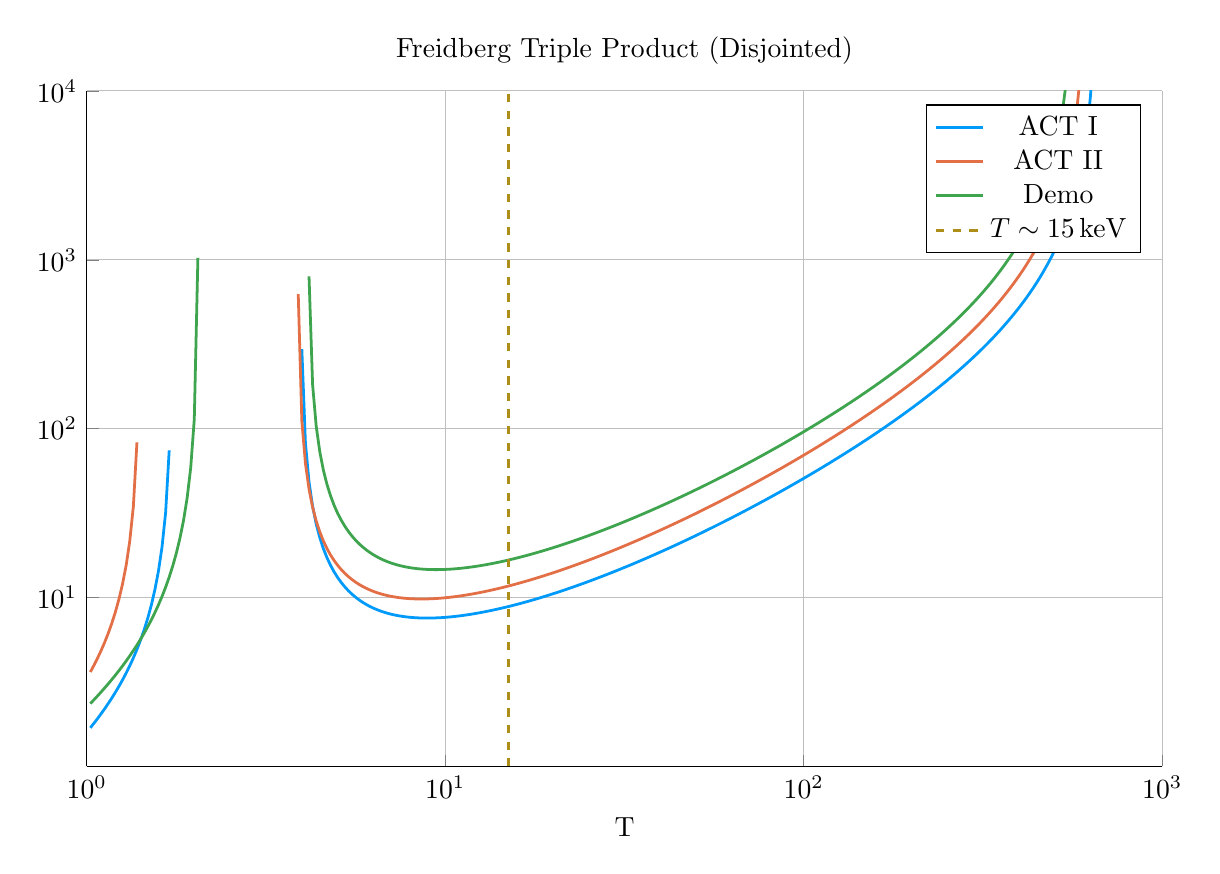
\begin{tikzpicture}[]
\begin{axis}[height = {101.6mm}, ylabel = {}, title = {Freidberg Triple Product (Disjointed)}, xmin = {1.0}, xmax = {1000.0}, ymax = {10000.0}, ymode = {log}, xlabel = {T}, {unbounded coords=jump, xticklabel style={rotate = 0}, log basis x=10, xmajorgrids = true, xtick = {1.0,10.0,100.0,1000.0}, xticklabels = {$10^{0}$,$10^{1}$,$10^{2}$,$10^{3}$}, xtick align = inside, axis lines* = left, yticklabel style={rotate = 0}, log basis y=10, ymajorgrids = true, ytick = {10.0,100.0,1000.0,10000.0}, yticklabels = {$10^{1}$,$10^{2}$,$10^{3}$,$10^{4}$}, ytick align = inside, axis lines* = left,     xshift = 0.0mm,
    yshift = 0.0mm,
    axis background/.style={fill={rgb,1:red,1.00000000;green,1.00000000;blue,1.00000000}}
}, xmode = {log}, ymin = {1.001}, width = {152.4mm}]\addplot+ [color = {rgb,1:red,0.00000000;green,0.60560316;blue,0.97868012},
draw opacity=1.0,
line width=1,
solid,mark = none,
mark size = 2.0,
mark options = {
    color = {rgb,1:red,0.00000000;green,0.00000000;blue,0.00000000}, draw opacity = 1.0,
    fill = {rgb,1:red,0.00000000;green,0.60560316;blue,0.97868012}, fill opacity = 1.0,
    line width = 1,
    rotate = 0,
    solid
}]coordinates {
(1.023292992280754, 1.6945150918881617)
(1.0471285480508996, 1.8022297212985727)
(1.0715193052376064, 1.9208400907418741)
(1.096478196143185, 2.0520379173824526)
(1.1220184543019633, 2.1978809957158)
(1.1481536214968828, 2.3608969492317664)
(1.1748975549395295, 2.5442241968703065)
(1.202264434617413, 2.7518066614453685)
(1.2302687708123816, 2.9886676965649497)
(1.2589254117941673, 3.2613035039971368)
(1.288249551693134, 3.5782615298822504)
(1.318256738556407, 3.9510138131485064)
(1.3489628825916535, 4.395316889582276)
(1.3803842646028848, 4.933406616196546)
(1.4125375446227544, 5.597693756447026)
(1.4454397707459274, 6.437310966298612)
(1.4791083881682074, 7.530455822814955)
(1.5135612484362082, 9.009551106277522)
(1.5488166189124815, 11.117997739838028)
(1.5848931924611136, 14.357045698731298)
(1.62181009735893, 19.94980446331863)
(1.6595869074375607, 31.870474474777332)
(1.6982436524617444, 74.50886497100848)
(1.7378008287493754, -268.62399052136783)
(1.7782794100389228, -49.919103932965776)
(1.8197008586099834, -28.182974323791697)
(1.8620871366628675, -19.98239680052841)
(1.9054607179632472, -15.70205772252279)
(1.9498445997580451, -13.093397062325929)
(1.9952623149688795, -11.354078520088276)
(2.041737944669529, -10.126703775296521)
(2.0892961308540396, -9.228291825900367)
(2.137962089502232, -8.555793230466092)
(2.1877616239495525, -8.047086394966504)
(2.2387211385683394, -7.662850026356773)
(2.290867652767773, -7.377360182440818)
(2.344228815319922, -7.173493942563709)
(2.3988329190194904, -7.03987823872135)
(2.4547089156850306, -6.969209177348767)
(2.51188643150958, -6.957252425128463)
(2.5703957827688635, -7.0022689551713535)
(2.6302679918953817, -7.104731798631218)
(2.6915348039269156, -7.2672686328905565)
(2.7542287033381663, -7.494810686078433)
(2.8183829312644537, -7.794966372176634)
(2.884031503126606, -8.178679918245468)
(2.9512092266663856, -8.661293939987127)
(3.019951720402016, -9.264230780294357)
(3.0902954325135905, -10.01767902164183)
(3.1622776601683795, -10.964999922356022)
(3.2359365692962827, -12.170236892008582)
(3.311311214825911, -13.7315665677587)
(3.3884415613920256, -15.806961575136446)
(3.4673685045253166, -18.667256898848134)
(3.548133892335755, -22.818098057023896)
(3.630780547701014, -29.323816090272153)
(3.715352290971725, -40.87190947609052)
(3.8018939632056115, -66.7704951710188)
(3.890451449942806, -176.00214091027135)
(3.9810717055349722, 296.2120048547568)
(4.073802778041127, 82.22608375442015)
(4.168693834703354, 48.43306336833725)
(4.265795188015927, 34.70962566295797)
(4.36515832240166, 27.295945016455207)
(4.466835921509632, 22.67019834453781)
(4.570881896148751, 19.52007287600256)
(4.677351412871983, 17.24499928723126)
(4.786300923226384, 15.531278040885976)
(4.897788193684462, 14.199095003080004)
(5.011872336272722, 13.138001469719821)
(5.1286138399136485, 12.27642393656205)
(5.248074602497725, 11.565956055783074)
(5.370317963702527, 10.972696881733755)
(5.495408738576246, 10.472204393849793)
(5.623413251903491, 10.04641840843593)
(5.7543993733715695, 9.681711040383625)
(5.88843655355589, 9.367610463946743)
(6.025595860743578, 9.095941481219963)
(6.165950018614822, 8.860232308719008)
(6.309573444801933, 8.655296117741381)
(6.456542290346556, 8.476930095683173)
(6.606934480075959, 8.321695258418004)
(6.760829753919817, 8.186752828259676)
(6.918309709189364, 8.06974093001644)
(7.079457843841379, 7.968680480243153)
(7.244359600749901, 7.881902520894599)
(7.413102413009175, 7.80799150193639)
(7.5857757502918375, 7.745740605469891)
(7.762471166286917, 7.694116194091195)
(7.943282347242816, 7.652229324407223)
(8.128305161640993, 7.619312722352829)
(8.31763771102671, 7.594702046961867)
(8.511380382023766, 7.577820541204338)
(8.709635899560805, 7.568166379774354)
(8.912509381337454, 7.565302179476453)
(9.120108393559097, 7.568846255848602)
(9.33254300796991, 7.57846529863635)
(9.549925860214358, 7.593868207120024)
(9.772372209558107, 7.614800878969009)
(10.0, 7.6410417872330525)
(10.232929922807541, 7.672398212107776)
(10.471285480508996, 7.708703019333509)
(10.715193052376065, 7.7498118970722105)
(10.964781961431852, 7.7956009790373795)
(11.220184543019636, 7.845964794420564)
(11.481536214968829, 7.9008144954472845)
(11.748975549395297, 7.960076321728849)
(12.02264434617413, 8.023690267358889)
(12.302687708123818, 8.091608922249174)
(12.589254117941675, 8.163796463753897)
(12.882495516931343, 8.240227778388245)
(13.182567385564074, 8.320887696558643)
(13.489628825916533, 8.405770325808698)
(13.803842646028846, 8.494878470244457)
(14.12537544622754, 8.588223125611163)
(14.454397707459272, 8.68582304101473)
(14.791083881682072, 8.787704339563915)
(15.13561248436208, 8.893900191356126)
(15.488166189124811, 9.00445053273945)
(15.848931924611133, 9.119401827772037)
(16.218100973589298, 9.238806866525163)
(16.595869074375607, 9.36272459734332)
(16.982436524617444, 9.49121998943775)
(17.378008287493753, 9.62436392387273)
(17.78279410038923, 9.762233108678469)
(18.197008586099834, 9.904910018476908)
(18.620871366628677, 10.052482855035347)
(19.054607179632473, 10.205045527912834)
(19.498445997580454, 10.362697653760055)
(19.952623149688797, 10.525544573138253)
(20.417379446695296, 10.693697383890798)
(20.892961308540396, 10.86727299025056)
(21.379620895022324, 11.04639416699954)
(21.87761623949553, 11.231189638117145)
(22.3872113856834, 11.42179416946176)
(22.908676527677734, 11.6183486751283)
(23.442288153199225, 11.82100033721453)
(23.9883291901949, 12.029902739089)
(24.547089156850298, 12.245216010109123)
(25.118864315095795, 12.467106987583263)
(25.703957827688633, 12.695749386290691)
(26.302679918953814, 12.931323985371597)
(26.915348039269155, 13.174018826913404)
(27.542287033381662, 13.424029428392666)
(28.183829312644534, 13.681559008968577)
(28.84031503126606, 13.946818729958853)
(29.512092266663856, 14.220027949885045)
(30.19951720402016, 14.50141449453101)
(30.902954325135905, 14.791214942515055)
(31.622776601683793, 15.089674926934103)
(32.359365692962825, 15.39704945369735)
(33.11311214825911, 15.713603237227478)
(33.884415613920254, 16.039611054270374)
(34.673685045253166, 16.375358304735574)
(35.48133892335755, 16.72114046362978)
(36.30780547701014, 17.077265375464844)
(37.15352290971726, 17.444051808101882)
(38.018939632056124, 17.821830851190978)
(38.90451449942807, 18.210946209955225)
(39.810717055349734, 18.611754712404426)
(40.73802778041128, 19.02462684323082)
(41.68693834703355, 19.44994730585631)
(42.65795188015925, 19.888115614110824)
(43.65158322401658, 20.33954671581207)
(44.6683592150963, 20.804671648648)
(45.708818961487495, 21.283938232164516)
(46.77351412871981, 21.777811796588267)
(47.86300923226383, 22.286775951266307)
(48.97788193684461, 22.811333395047512)
(50.11872336272722, 23.352006771196773)
(51.28613839913648, 23.90933956979331)
(52.48074602497726, 24.483897079598876)
(53.70317963702527, 25.07626739512277)
(54.954087385762456, 25.687062479009892)
(56.23413251903491, 26.316919285823328)
(57.543993733715695, 26.966500951119475)
(58.8843655355589, 27.63649804806381)
(60.25595860743578, 28.32762991928082)
(61.65950018614822, 29.040646086657393)
(63.09573444801933, 29.776327745458484)
(64.56542290346556, 30.535489348458338)
(66.06934480075961, 31.318980286421752)
(67.60829753919819, 32.12768667178653)
(69.18309709189366, 32.96253323296315)
(70.79457843841381, 33.82448532728458)
(72.44359600749902, 34.71455108131369)
(74.13102413009177, 35.63378366795554)
(75.85775750291836, 36.5832837306308)
(77.62471166286916, 37.56420196565578)
(79.43282347242814, 38.5777418749493)
(81.2830516164099, 39.625162702259914)
(83.17637711026708, 40.70778256728596)
(85.11380382023764, 41.82698181336084)
(87.09635899560806, 42.98420658580859)
(89.12509381337455, 44.18097265965641)
(91.20108393559097, 45.41886953713795)
(93.3254300796991, 46.69956483735465)
(95.49925860214358, 48.0248090026031)
(97.72372209558107, 49.39644034825024)
(100.0, 50.81639048567384)
(102.32929922807536, 52.28669015071427)
(104.71285480508996, 53.809475473344484)
(107.1519305237606, 55.38699472789598)
(109.64781961431851, 57.02161560723521)
(112.2018454301963, 58.71583306880927)
(114.81536214968828, 60.47227780555281)
(117.48975549395291, 62.29372540032026)
(120.22644346174131, 64.1831062288853)
(123.02687708123811, 66.14351618370313)
(125.89254117941675, 68.17822829869775)
(128.82495516931337, 70.29070536425795)
(131.82567385564073, 72.48461363302665)
(134.89628825916532, 74.76383772515437)
(138.03842646028852, 77.13249686084183)
(141.2537544622754, 79.59496255677749)
(144.5439770745928, 82.1558779437945)
(147.91083881682073, 84.82017888112068)
(151.35612484362088, 87.59311706484252)
(154.88166189124811, 90.48028535342075)
(158.48931924611142, 93.48764556200553)
(162.18100973589299, 96.62155901048361)
(165.95869074375614, 99.88882014839527)
(169.82436524617444, 103.29669362390514)
(173.78008287493762, 106.8529552149526)
(177.82794100389228, 110.56593709971621)
(181.97008586099827, 114.44457801209604)
(186.20871366628674, 118.49847890775631)
(190.54607179632464, 122.73796485951151)
(194.98445997580455, 127.17415401000369)
(199.52623149688787, 131.81903453779776)
(204.17379446695296, 136.68555074397534)
(208.92961308540387, 141.7876995445982)
(213.79620895022325, 147.14063886569335)
(218.77616239495518, 152.76080968855555)
(223.872113856834, 158.66607379276888)
(229.08676527677724, 164.87586960296383)
(234.42288153199226, 171.4113889762298)
(239.88329190194898, 178.29577828677515)
(245.4708915685031, 185.55436779375145)
(251.18864315095797, 193.21493404336246)
(257.03957827688646, 201.30800099096868)
(263.02679918953817, 209.86718667547356)
(269.1534803926917, 218.92960369175984)
(275.4228703338166, 228.5363234580894)
(281.8382931264455, 238.73291645637224)
(288.40315031266056, 249.57008335444863)
(295.1209226666387, 261.10439535985074)
(301.9951720402016, 273.39916651425244)
(309.0295432513592, 286.52548620009975)
(316.22776601683796, 300.5634472677593)
(323.5936569296281, 315.60361443723326)
(331.1311214825911, 331.74878965791873)
(338.84415613920237, 349.11614693461144)
(346.73685045253166, 367.83983008944125)
(354.8133892335753, 388.074134968045)
(363.0780547701014, 409.9974354672692)
(371.5352290971724, 433.8170644462405)
(380.1893963205613, 459.775431919879)
(389.04514499428046, 488.15776259296996)
(398.1071705534973, 519.301975844092)
(407.3802778041126, 553.6114337377378)
(416.8693834703355, 591.5715777555781)
(426.57951880159254, 633.7719123174471)
(436.5158322401661, 680.9354532594568)
(446.683592150963, 733.9587765720896)
(457.0881896148752, 793.9674013286159)
(467.73514128719813, 862.3938269620526)
(478.6300923226385, 941.0898231518593)
(489.77881936844614, 1032.4918995815904)
(501.18723362727246, 1139.8718558647272)
(512.8613839913648, 1267.728232380304)
(524.8074602497728, 1422.4206670383826)
(537.0317963702527, 1613.2432940240717)
(549.5408738576248, 1854.3379168248518)
(562.341325190349, 2168.328384373693)
(575.4399373371566, 2593.8014145005036)
(588.843655355589, 3202.400412559708)
(602.5595860743575, 4143.871725688599)
(616.5950018614822, 5792.368998792458)
(630.957344480193, 9418.65571693456)
(645.6542290346556, 23889.28171950775)
(660.6934480075957, -49140.70577934398)
(676.0829753919819, -12421.08556602776)
(691.8309709189363, -7211.5383604203)
(707.945784384138, -5131.503513512916)
(724.4359600749899, -4013.149779314024)
(741.3102413009177, -3315.290437938855)
(758.5775750291835, -2838.6775691444445)
(776.247116628692, -2492.7815835486012)
(794.3282347242813, -2230.5404344031062)
(812.8305161640995, -2025.0671265994276)
(831.7637711026708, -1859.8852065397507)
(851.1380382023768, -1724.3348515292655)
(870.9635899560806, -1611.214292586841)
(891.2509381337459, -1515.482798133364)
(912.0108393559096, -1433.5066904171208)
(933.2543007969915, -1362.60044755666)
(954.992586021436, -1300.7364064371823)
(977.2372209558112, -1246.3549673169614)
(1000.0, -1198.236922422159)
(1023.2929922807537, -1155.4154111586524)
(1047.1285480508996, -1117.1138595692732)
(1071.519305237606, -1082.7013755947412)
(1096.4781961431852, -1051.6601296512954)
(1122.018454301963, -1023.5611236164838)
(1148.1536214968828, -998.0459352192751)
(1174.897554939529, -974.8127865165062)
(1202.2644346174131, -953.6057869052796)
(1230.268770812381, -934.2065376059747)
(1258.9254117941675, -916.427514142416)
(1288.2495516931335, -900.1068024887031)
(1318.2567385564075, -885.1038764728944)
(1348.9628825916532, -871.2961837984906)
(1380.3842646028852, -858.5763656093441)
(1412.537544622754, -846.8499765447623)
(1445.439770745928, -836.0336032365552)
(1479.1083881682073, -826.0533023067777)
(1513.5612484362086, -816.8432963076928)
(1548.816618912481, -808.3448792375339)
(1584.893192461114, -800.5054933601936)
(1621.8100973589299, -793.2779468416144)
(1659.5869074375614, -786.619747763086)
(1698.2436524617442, -780.4925348022881)
(1737.8008287493763, -774.8615885976767)
(1778.2794100389228, -769.695410762998)
(1819.7008586099826, -764.9653598706944)
(1862.0871366628676, -760.6453356042871)
(1905.4607179632462, -756.7115038241651)
(1949.8445997580454, -753.1420564513764)
(1995.2623149688789, -749.9170011631115)
(2041.7379446695295, -747.017976692142)
(2089.296130854039, -744.4280901019075)
(2137.9620895022326, -742.1317730997671)
(2187.761623949552, -740.1146548191589)
(2238.72113856834, -738.3634489135239)
(2290.8676527677726, -736.8658531085748)
(2344.228815319923, -735.6104596965912)
(2398.83291901949, -734.5866754712753)
(2454.708915685031, -733.7846501343085)
(2511.88643150958, -733.1952120249796)
(2570.3957827688646, -732.8098103606878)
(2630.2679918953813, -732.6204632251878)
(2691.5348039269165, -732.619710649065)
(2754.2287033381663, -732.8005722110505)
(2818.382931264455, -733.1565086609373)
(2884.031503126606, -733.6813871269079)
(2951.209226666387, -734.3694495236135)
(3019.9517204020162, -735.2152838235631)
(3090.295432513592, -736.2137978944917)
(3162.2776601683795, -737.3601956401093)
(3235.936569296281, -738.6499552119711)
(3311.311214825911, -740.0788090865385)
(3388.441561392024, -741.6427258246325)
(3467.368504525317, -743.3378933506358)
(3548.133892335753, -745.1607036065371)
(3630.780547701014, -747.1077384514889)
(3715.352290971724, -749.1757566912511)
(3801.8939632056126, -751.3616821340012)
(3890.4514499428046, -753.6625925796814)
(3981.0717055349733, -756.0757096595084)
(4073.802778041126, -758.5983894506668)
(4168.693834703355, -761.2281137986595)
(4265.795188015925, -763.9624822864063)
(4365.158322401661, -766.7992045807192)
(4466.835921509631, -769.7360946070586)
(4570.881896148751, -772.7710620056145)
(4677.351412871981, -775.9021083311076)
(4786.300923226385, -779.1273204560445)
(4897.7881936844615, -782.4448656456962)
(5011.872336272725, -785.8529867735253)
(5128.613839913648, -789.3499978635558)
(5248.074602497728, -792.9342799342446)
(5370.317963702527, -796.604277116354)
(5495.408738576249, -800.3584930490041)
(5623.413251903491, -804.195487472099)
(5754.399373371566, -808.1138730792338)
(5888.43655355589, -812.1123125544108)
(6025.595860743575, -816.1895158014244)
(6165.9500186148225, -820.3442373483241)
(6309.57344480193, -824.575273914367)
(6456.542290346556, -828.8814621278906)
(6606.934480075957, -833.2616763844619)
(6760.829753919818, -837.7148268354883)
(6918.309709189362, -842.2398574982564)
(7079.457843841381, -846.8357444790493)
(7244.359600749898, -851.5014943016532)
(7413.102413009177, -856.2361423341288)
(7585.775750291836, -861.0387513072818)
(7762.4711662869195, -865.9084099187404)
(7943.282347242814, -870.8442315170112)
(8128.305161640995, -875.8453528602984)
(8317.63771102671, -880.9109329452398)
(8511.380382023768, -886.0401519010943)
(8709.635899560806, -891.2322099451943)
(8912.509381337459, -896.4863263958177)
(9120.108393559096, -901.8017387388758)
(9332.543007969914, -907.1777017450888)
(9549.92586021436, -912.6134865547074)
(9772.372209558112, -918.1083801920363)
(10000.0, -923.6616844862497)
};
\addlegendentry{ACT I}
\addplot+ [color = {rgb,1:red,0.88887350;green,0.43564919;blue,0.27812294},
draw opacity=1.0,
line width=1,
solid,mark = none,
mark size = 2.0,
mark options = {
    color = {rgb,1:red,0.00000000;green,0.00000000;blue,0.00000000}, draw opacity = 1.0,
    fill = {rgb,1:red,0.88887350;green,0.43564919;blue,0.27812294}, fill opacity = 1.0,
    line width = 1,
    rotate = 0,
    solid
}]coordinates {
(1.023292992280754, 3.6262198595749764)
(1.0471285480508996, 3.9709951177889846)
(1.0715193052376064, 4.3756174014389835)
(1.096478196143185, 4.856923072933348)
(1.1220184543019633, 5.438683072221177)
(1.1481536214968828, 6.155573870975628)
(1.1748975549395295, 7.060228008162098)
(1.202264434617413, 8.236563724204407)
(1.2302687708123816, 9.827054231195484)
(1.2589254117941673, 12.094532497587037)
(1.288249551693134, 15.583209353705142)
(1.318256738556407, 21.63257843385939)
(1.3489628825916535, 34.66570824747554)
(1.3803842646028848, 83.08790958003418)
(1.4125375446227544, -237.94957827646257)
(1.4454397707459274, -50.355280711590225)
(1.4791083881682074, -28.63496801892399)
(1.5135612484362082, -20.251666213285585)
(1.5488166189124815, -15.820177297479631)
(1.5848931924611136, -13.08951908492532)
(1.62181009735893, -11.24674808778935)
(1.6595869074375607, -9.926910662341783)
(1.6982436524617444, -8.941965953571943)
(1.7378008287493754, -8.185314268502955)
(1.7782794100389228, -7.592149139482488)
(1.8197008586099834, -7.120936958963385)
(1.8620871366628675, -6.74396430844709)
(1.9054607179632472, -6.442168044456181)
(1.9498445997580451, -6.202147460832283)
(1.9952623149688795, -6.014359309768401)
(2.041737944669529, -5.871988456076733)
(2.0892961308540396, -5.770222564971642)
(2.137962089502232, -5.705778915745288)
(2.1877616239495525, -5.676595450141278)
(2.2387211385683394, -5.68163408082953)
(2.290867652767773, -5.720765456471678)
(2.344228815319922, -5.794717627708497)
(2.3988329190194904, -5.9050800796980125)
(2.4547089156850306, -6.054361567255678)
(2.51188643150958, -6.246106580679075)
(2.5703957827688635, -6.485082333271136)
(2.6302679918953817, -6.777557290905968)
(2.6915348039269156, -7.1317054161224025)
(2.7542287033381663, -7.558190626573394)
(2.8183829312644537, -8.071018969252556)
(2.884031503126606, -8.688801804272321)
(2.9512092266663856, -9.436671353402025)
(3.019951720402016, -10.349269580424053)
(3.0902954325135905, -11.475575910838932)
(3.1622776601683795, -12.887036452859418)
(3.2359365692962827, -14.691959839828085)
(3.311311214825911, -17.06263857450721)
(3.3884415613920256, -20.29057894681975)
(3.4673685045253166, -24.910913722214016)
(3.548133892335755, -32.02376727816436)
(3.630780547701014, -44.30667919768318)
(3.715352290971725, -70.4202182892387)
(3.8018939632056115, -162.8647166076088)
(3.890451449942806, 626.9103884763274)
(3.9810717055349722, 111.1855857788192)
(4.073802778041127, 62.30641416623654)
(4.168693834703354, 43.93800066040291)
(4.265795188015927, 34.33706014393487)
(4.36515832240166, 28.454603024787982)
(4.466835921509632, 24.493996588522855)
(4.570881896148751, 21.655444964297164)
(4.677351412871983, 19.528883534080794)
(4.786300923226384, 17.882391475312325)
(4.897788193684462, 16.574948455957568)
(5.011872336272722, 15.51588818674524)
(5.1286138399136485, 14.644277005698534)
(5.248074602497725, 13.917659005030185)
(5.370317963702527, 13.305553561598769)
(5.495408738576246, 12.785518065105022)
(5.623413251903491, 12.340668088629867)
(5.7543993733715695, 11.958062188819154)
(5.88843655355589, 11.627618960477479)
(6.025595860743578, 11.341372389870859)
(6.165950018614822, 11.092948328333481)
(6.309573444801933, 10.877189105947096)
(6.456542290346556, 10.689879592932128)
(6.606934480075959, 10.527544110660646)
(6.760829753919817, 10.387293705403508)
(6.918309709189364, 10.266709799369176)
(7.079457843841379, 10.16375450253595)
(7.244359600749901, 10.076700725700801)
(7.413102413009175, 10.004077180609906)
(7.5857757502918375, 9.944624699045534)
(7.762471166286917, 9.897261247744884)
(7.943282347242816, 9.861053688507223)
(8.128305161640993, 9.835194817415095)
(8.31763771102671, 9.818984570337387)
(8.511380382023766, 9.811814542185662)
(8.709635899560805, 9.813155162447515)
(8.912509381337454, 9.822545006156611)
(9.120108393559097, 9.83958185650335)
(9.33254300796991, 9.863915174108707)
(9.549925860214358, 9.895239747025146)
(9.772372209558107, 9.933290289132369)
(10.0, 9.977836853773296)
(10.232929922807541, 10.028680908432321)
(10.471285480508996, 10.085651971057402)
(10.715193052376065, 10.148604718433416)
(10.964781961431852, 10.21741649362127)
(11.220184543019636, 10.291985152574611)
(11.481536214968829, 10.37222719997026)
(11.748975549395297, 10.458076172688434)
(12.02264434617413, 10.549481236152369)
(12.302687708123818, 10.64640596430817)
(12.589254117941675, 10.748827278619041)
(12.882495516931343, 10.856734525250282)
(13.182567385564074, 10.970128672782435)
(13.489628825916533, 11.089021615426763)
(13.803842646028846, 11.213435568926192)
(14.12537544622754, 11.343402548181452)
(14.454397707459272, 11.478963917208173)
(14.791083881682072, 11.620170003356527)
(15.13561248436208, 11.767079768850763)
(15.488166189124811, 11.919760533665668)
(15.848931924611133, 12.078287744603548)
(16.218100973589298, 12.242744785962834)
(16.595869074375607, 12.413222828300148)
(16.982436524617444, 12.589820711506782)
(17.378008287493753, 12.772644859640952)
(17.78279410038923, 12.961809224911852)
(18.197008586099834, 13.157435258695006)
(18.620871366628677, 13.359651907740494)
(19.054607179632473, 13.568595633881658)
(19.498445997580454, 13.78441045660099)
(19.952623149688797, 14.007248015617566)
(20.417379446695296, 14.237267654769363)
(20.892961308540396, 14.474636524779191)
(21.379620895022324, 14.719529704908814)
(21.87761623949553, 14.972130342899538)
(22.3872113856834, 15.232629812825081)
(22.908676527677734, 15.501227890845222)
(23.442288153199225, 15.778132947219865)
(23.9883291901949, 16.06356215819839)
(24.547089156850298, 16.35774173268541)
(25.118864315095795, 16.660907159108888)
(25.703957827688633, 16.973303467018464)
(26.302679918953814, 17.295185509573656)
(26.915348039269155, 17.62681826308181)
(27.542287033381662, 17.96847714569595)
(28.183829312644534, 18.32044835551375)
(28.84031503126606, 18.6830292286709)
(29.512092266663856, 19.05652861809976)
(30.19951720402016, 19.441267293702094)
(30.902954325135905, 19.837578364764788)
(31.622776601683793, 20.245807725529637)
(32.359365692962825, 20.66631452491334)
(33.11311214825911, 21.099471661462132)
(33.884415613920254, 21.54566630471813)
(34.673685045253166, 22.00530044427105)
(35.48133892335755, 22.47879146787113)
(36.30780547701014, 22.966572770086653)
(37.15352290971726, 23.469094393103948)
(38.018939632056124, 23.986823701388534)
(38.90451449942807, 24.520246092055554)
(39.810717055349734, 25.069865742935068)
(40.73802778041128, 25.636206400465333)
(41.68693834703355, 26.219812206925383)
(42.65795188015925, 26.82124858892035)
(43.65158322401658, 27.441103151399624)
(44.6683592150963, 28.079986677312778)
(45.708818961487495, 28.73853413868146)
(46.77351412871981, 29.417405780721598)
(47.86300923226383, 30.117288263079946)
(48.97788193684461, 30.838895864745762)
(50.11872336272722, 31.582971756705206)
(51.28613839913648, 32.35028934671438)
(52.48074602497726, 33.14165370090234)
(53.70317963702527, 33.957903047277725)
(54.954087385762456, 34.79991036660676)
(56.23413251903491, 35.668585076557704)
(57.543993733715695, 36.56487481530732)
(58.8843655355589, 37.4897673324607)
(60.25595860743578, 38.44429249224886)
(61.65950018614822, 39.42952440027207)
(63.09573444801933, 40.44658366003865)
(64.56542290346556, 41.496639769647544)
(66.06934480075961, 42.58091366862388)
(67.60829753919819, 43.70068044592992)
(69.18309709189366, 44.857272221109575)
(70.79457843841381, 46.052081211550274)
(72.44359600749902, 47.286562999969696)
(74.13102413009177, 48.562240017471)
(75.85775750291836, 49.8807052588659)
(77.62471166286916, 51.243626248459464)
(79.43282347242814, 52.65274927613318)
(81.2830516164099, 54.10990392537751)
(83.17637711026708, 55.617007916924386)
(85.11380382023764, 57.17607229384146)
(87.09635899560806, 58.78920697639489)
(89.12509381337455, 60.458626717694976)
(91.20108393559097, 62.18665749414143)
(93.3254300796991, 63.97574336801635)
(95.49925860214358, 65.82845386036456)
(97.72372209558107, 67.74749189972668)
(100.0, 69.73570233531223)
(102.32929922807536, 71.79608117146411)
(104.71285480508996, 73.93178548206338)
(107.1519305237606, 76.14614413306579)
(109.64781961431851, 78.44266936696852)
(112.2018454301963, 80.8250693343548)
(114.81536214968828, 83.29726166380183)
(117.48975549395291, 85.86338817160895)
(120.22644346174131, 88.52783082428154)
(123.02687708123811, 91.29522907965378)
(125.89254117941675, 94.17049874718609)
(128.82495516931337, 97.15885252455993)
(131.82567385564073, 100.26582238652995)
(134.89628825916532, 103.497284023392)
(138.03842646028852, 106.8594835506073)
(141.2537544622754, 110.35906674040386)
(144.5439770745928, 114.00311105358536)
(147.91083881682073, 117.79916079358593)
(151.35612484362088, 121.75526573929804)
(154.88166189124811, 125.88002366576029)
(158.48931924611142, 130.1826272158626)
(162.18100973589299, 134.672915650604)
(165.95869074375614, 139.36143207981326)
(169.82436524617444, 144.25948686159074)
(173.78008287493762, 149.37922795930874)
(177.82794100389228, 154.73371916238966)
(181.97008586099827, 160.33702721452812)
(186.20871366628674, 166.20431905434293)
(190.54607179632464, 172.35197056339555)
(194.98445997580455, 178.79768844082054)
(199.52623149688787, 185.56064708952624)
(204.17379446695296, 192.66164271474446)
(208.92961308540387, 200.12326721230153)
(213.79620895022325, 207.97010486869286)
(218.77616239495518, 216.2289554844475)
(223.872113856834, 224.92908801677567)
(229.08676527677724, 234.10252996410594)
(234.42288153199226, 243.78439825504503)
(239.88329190194898, 254.013278913416)
(245.4708915685031, 264.831664041007)
(251.18864315095797, 276.2864564799751)
(257.03957827688646, 288.42955470570877)
(263.02679918953817, 301.31853323333485)
(269.1534803926917, 315.01743724146417)
(275.4228703338166, 329.5977144230688)
(281.8382931264455, 345.13931252826)
(288.40315031266056, 361.7319780177609)
(295.1209226666387, 379.47680017147866)
(301.9951720402016, 398.48805653482157)
(309.0295432513592, 418.8954306148157)
(316.22776601683796, 440.8466924729332)
(323.5936569296281, 464.5109589979699)
(331.1311214825911, 490.0826855730525)
(338.84415613920237, 517.7865879974996)
(346.73685045253166, 547.8837577991267)
(354.8133892335753, 580.6793227491402)
(363.0780547701014, 616.5321281016747)
(371.5352290971724, 655.8670890363044)
(380.1893963205613, 699.1911156139116)
(389.04514499428046, 747.1138767235202)
(398.1071705534973, 800.3752099841976)
(407.3802778041126, 859.8817991675508)
(416.8693834703355, 926.7569931156614)
(426.57951880159254, 1002.409608394075)
(436.5158322401661, 1088.6307275063882)
(446.683592150963, 1187.7327493644536)
(457.0881896148752, 1302.7538970715893)
(467.73514128719813, 1437.7671929229414)
(478.6300923226385, 1598.3619531251416)
(489.77881936844614, 1792.4217156957561)
(501.18723362727246, 2031.435864125701)
(512.8613839913648, 2332.8272604727294)
(524.8074602497728, 2724.3501891507594)
(537.0317963702527, 3253.0808589923313)
(549.5408738576248, 4005.7745115556468)
(562.341325190349, 5161.830905458572)
(575.4399373371566, 7161.999955047848)
(588.843655355589, 11456.916643900393)
(602.5595860743575, 27278.085748054084)
(616.5950018614822, -81374.99567859212)
(630.957344480193, -16777.758330681536)
(645.6542290346556, -9494.611990167594)
(660.6934480075957, -6689.456467425088)
(676.0829753919819, -5204.544925417548)
(691.8309709189363, -4286.084695387924)
(707.945784384138, -3662.3824611701343)
(724.4359600749899, -3211.5569830118793)
(741.3102413009177, -2870.7907078330154)
(758.5775750291835, -2604.4181322887152)
(776.247116628692, -2390.6863963037536)
(794.3282347242813, -2215.5742233715514)
(812.8305161640995, -2069.6372672190055)
(831.7637711026708, -1946.2815219657975)
(851.1380382023768, -1840.7635003469652)
(870.9635899560806, -1749.5836745614658)
(891.2509381337459, -1670.1038187095141)
(912.0108393559096, -1600.2974165784447)
(933.2543007969915, -1538.5821079233035)
(954.992586021436, -1483.704347654581)
(977.2372209558112, -1434.6582328197553)
(1000.0, -1390.6272443725638)
(1023.2929922807537, -1350.9416958920935)
(1047.1285480508996, -1315.0471613093978)
(1071.519305237606, -1282.4807127947604)
(1096.4781961431852, -1252.8528041238237)
(1122.018454301963, -1225.8332942321483)
(1148.1536214968828, -1201.1405477147484)
(1174.897554939529, -1178.5328496873165)
(1202.2644346174131, -1157.8015815679175)
(1230.268770812381, -1138.765750110663)
(1258.9254117941675, -1121.267566697522)
(1288.2495516931335, -1105.1688489426283)
(1318.2567385564075, -1090.348071514546)
(1348.9628825916532, -1076.6979335079102)
(1380.3842646028852, -1064.1233398013928)
(1412.537544622754, -1052.539716470997)
(1445.439770745928, -1041.8715974920947)
(1479.1083881682073, -1032.0514330898977)
(1513.5612484362086, -1023.018580214714)
(1548.816618912481, -1014.7184434731793)
(1584.893192461114, -1007.1017409878611)
(1621.8100973589299, -1000.1238744907862)
(1659.5869074375614, -993.744386783934)
(1698.2436524617442, -987.9264927488415)
(1737.8008287493763, -982.636672530169)
(1778.2794100389228, -977.8443174854673)
(1819.7008586099826, -973.5214210860804)
(1862.0871366628676, -969.6423082497454)
(1905.4607179632462, -966.1833976443339)
(1949.8445997580454, -963.1229923714116)
(1995.2623149688789, -960.4410951549132)
(2041.7379446695295, -958.1192447533882)
(2089.296130854039, -956.1403708072178)
(2137.9620895022326, -954.4886644127564)
(2187.761623949552, -953.1494647041984)
(2238.72113856834, -952.1091527568241)
(2290.8676527677726, -951.3550628814313)
(2344.228815319923, -950.8753984451814)
(2398.83291901949, -950.6591580412987)
(2454.708915685031, -950.6960687224226)
(2511.88643150958, -950.976525783883)
(2570.3957827688646, -951.4915383610024)
(2630.2679918953813, -952.2326801933348)
(2691.5348039269165, -953.1920450178479)
(2754.2287033381663, -954.3622060364678)
(2818.382931264455, -955.7361791027337)
(2884.031503126606, -957.3073891869254)
(2951.209226666387, -959.0696398044653)
(3019.9517204020162, -961.0170851050241)
(3090.295432513592, -963.1442043574473)
(3162.2776601683795, -965.4457785953113)
(3235.936569296281, -967.9168692139419)
(3311.311214825911, -970.5527983325226)
(3388.441561392024, -973.3491307549663)
(3467.368504525317, -976.301657380888)
(3548.133892335753, -979.406379933558)
(3630.780547701014, -982.6594968855042)
(3715.352290971724, -986.0573904745661)
(3801.8939632056126, -989.5966147140405)
(3890.4514499428046, -993.2738843101055)
(3981.0717055349733, -997.0860644082568)
(4073.802778041126, -1001.030161098068)
(4168.693834703355, -1005.1033126123773)
(4265.795188015925, -1009.3027811630325)
(4365.158322401661, -1013.6259453607602)
(4466.835921509631, -1018.0702931715625)
(4570.881896148751, -1022.633415366397)
(4677.351412871981, -1027.3129994248159)
(4786.300923226385, -1032.1068237614704)
(4897.7881936844615, -1037.0127529096899)
(5011.872336272725, -1042.0287316317933)
(5128.613839913648, -1047.1527812631514)
(5248.074602497728, -1052.3829949308802)
(5370.317963702527, -1057.7175336249259)
(5495.408738576249, -1063.1546224338358)
(5623.413251903491, -1068.6925470213334)
(5754.399373371566, -1074.3296503261488)
(5888.43655355589, -1080.0643294689673)
(6025.595860743575, -1085.8950328516705)
(6165.9500186148225, -1091.8202574352306)
(6309.57344480193, -1097.8385461836895)
(6456.542290346556, -1103.9484856626516)
(6606.934480075957, -1110.1487037816134)
(6760.829753919818, -1116.437867667452)
(6918.309709189362, -1122.8146816767116)
(7079.457843841381, -1129.2778854970907)
(7244.359600749898, -1135.8262523843705)
(7413.102413009177, -1142.4585874877714)
(7585.775750291836, -1149.1737262727324)
(7762.4711662869195, -1155.9705330323777)
(7943.282347242814, -1162.847899481954)
(8128.305161640995, -1169.8047434309324)
(8317.63771102671, -1176.840007527851)
(8511.380382023768, -1183.9526580733384)
(8709.635899560806, -1191.141683897054)
(8912.509381337459, -1198.4060952946172)
(9120.108393559096, -1205.7449230208424)
(9332.543007969914, -1213.1572173358775)
(9549.92586021436, -1220.642047101055)
(9772.372209558112, -1228.198498921507)
(10000.0, -1235.8256763101228)
};
\addlegendentry{ACT II}
\addplot+ [color = {rgb,1:red,0.24222430;green,0.64327509;blue,0.30444865},
draw opacity=1.0,
line width=1,
solid,mark = none,
mark size = 2.0,
mark options = {
    color = {rgb,1:red,0.00000000;green,0.00000000;blue,0.00000000}, draw opacity = 1.0,
    fill = {rgb,1:red,0.24222430;green,0.64327509;blue,0.30444865}, fill opacity = 1.0,
    line width = 1,
    rotate = 0,
    solid
}]coordinates {
(1.023292992280754, 2.35717971253544)
(1.0471285480508996, 2.4818091803011884)
(1.0715193052376064, 2.6160533994079267)
(1.096478196143185, 2.7610169738489345)
(1.1220184543019633, 2.9179792560669826)
(1.1481536214968828, 3.088429876891961)
(1.1748975549395295, 3.2741132141278877)
(1.202264434617413, 3.4770845203202887)
(1.2302687708123816, 3.6997814161989337)
(1.2589254117941673, 3.9451158626625746)
(1.288249551693134, 4.216593759892962)
(1.318256738556407, 4.5184723163672)
(1.3489628825916535, 4.8559698120095405)
(1.3803842646028848, 5.235549216958988)
(1.4125375446227544, 5.6653077812466694)
(1.4454397707459274, 6.155521704098852)
(1.4791083881682074, 6.719422812007362)
(1.5135612484362082, 7.374331069416676)
(1.5488166189124815, 8.143348442005678)
(1.5848931924611136, 9.0579674025362)
(1.62181009735893, 10.162226448053275)
(1.6595869074375607, 11.51959922678817)
(1.6982436524617444, 13.224971744537322)
(1.7378008287493754, 15.426704428972686)
(1.7782794100389228, 18.37029833004982)
(1.8197008586099834, 22.493152913401733)
(1.8620871366628675, 28.65703826424774)
(1.9054607179632472, 38.826389394454985)
(1.9498445997580451, 58.65838956889421)
(1.9952623149688795, 113.86026736745272)
(2.041737944669529, 1028.465896265156)
(2.0892961308540396, -156.98955302050203)
(2.137962089502232, -75.58944517456705)
(2.1877616239495525, -51.04391619634808)
(2.2387211385683394, -39.30966054980392)
(2.290867652767773, -32.5119531577225)
(2.344228815319922, -28.143264194500333)
(2.3988329190194904, -25.158071654062468)
(2.4547089156850306, -23.0445846464956)
(2.51188643150958, -21.52440818514324)
(2.5703957827688635, -20.43488629677609)
(2.6302679918953817, -19.676536809340007)
(2.6915348039269156, -19.18724883626914)
(2.7542287033381663, -18.92875930297599)
(2.8183829312644537, -18.87930979578657)
(2.884031503126606, -19.02971234594769)
(2.9512092266663856, -19.381519932557275)
(3.019951720402016, -19.946725352708658)
(3.0902954325135905, -20.74884656063491)
(3.1622776601683795, -21.825612263340254)
(3.2359365692962827, -23.233892020991846)
(3.311311214825911, -25.05821583556076)
(3.3884415613920256, -27.425575246468597)
(3.4673685045253166, -30.532068258328167)
(3.548133892335755, -34.6936386598954)
(3.630780547701014, -40.450370735740485)
(3.715352290971725, -48.803893211628264)
(3.8018939632056115, -61.839107568518806)
(3.890451449942806, -84.72360389451674)
(3.9810717055349722, -134.73071514219606)
(4.073802778041127, -326.7218117310164)
(4.168693834703354, 798.2884776786321)
(4.265795188015927, 182.0559821932355)
(4.36515832240166, 103.75476422947621)
(4.466835921509632, 73.15084324411494)
(4.570881896148751, 56.90014770917698)
(4.677351412871983, 46.86280231089802)
(4.786300923226384, 40.07409117664327)
(4.897788193684462, 35.19587156238823)
(5.011872336272722, 31.53573209180628)
(5.1286138399136485, 28.69950502793406)
(5.248074602497725, 26.446359733467812)
(5.370317963702527, 24.620894487256926)
(5.495408738576246, 23.11837741508691)
(5.623413251903491, 21.86567883944471)
(5.7543993733715695, 20.81020944532067)
(5.88843655355589, 19.91319942113111)
(6.025595860743578, 19.145453338573617)
(6.165950018614822, 18.484578493662337)
(6.309573444801933, 17.91312275369926)
(6.456542290346556, 17.417291943801875)
(6.606934480075959, 16.98604667476511)
(6.760829753919817, 16.610453971230086)
(6.918309709189364, 16.283213587869994)
(7.079457843841379, 15.998306518944684)
(7.244359600749901, 15.750730470203408)
(7.413102413009175, 15.536298211082281)
(7.5857757502918375, 15.351482055139172)
(7.762471166286917, 15.193292627587141)
(7.943282347242816, 15.059183429252593)
(8.128305161640993, 14.946975025647662)
(8.31763771102671, 14.854794320700986)
(8.511380382023766, 14.781025536184384)
(8.709635899560805, 14.7242703555862)
(8.912509381337454, 14.683315302358887)
(9.120108393559097, 14.65710487318027)
(9.33254300796991, 14.644719282590849)
(9.549925860214358, 14.645355927794705)
(9.772372209558107, 14.658313873881836)
(10.0, 14.682980806167361)
(10.232929922807541, 14.718822009214483)
(10.471285480508996, 14.765371019745997)
(10.715193052376065, 14.822221669168664)
(10.964781961431852, 14.889021285358137)
(11.220184543019636, 14.965464866053368)
(11.481536214968829, 15.05129007022395)
(11.748975549395297, 15.14627290102121)
(12.02264434617413, 15.25022397586703)
(12.302687708123818, 15.362985297092992)
(12.589254117941675, 15.484427450328177)
(12.882495516931343, 15.614447171583684)
(13.182567385564074, 15.752965230502607)
(13.489628825916533, 15.899924588336324)
(13.803842646028846, 16.055288793998695)
(14.12537544622754, 16.219040587639775)
(14.454397707459272, 16.391180685479707)
(14.791083881682072, 16.571726724885952)
(15.13561248436208, 16.760712347737194)
(15.488166189124811, 16.95818640970398)
(15.848931924611133, 17.164212298589476)
(16.218100973589298, 17.378867350854325)
(16.595869074375607, 17.60224235578842)
(16.982436524617444, 17.834441138402067)
(17.378008287493753, 18.075580213329598)
(17.78279410038923, 18.325788503087594)
(18.197008586099834, 18.58520711493611)
(18.620871366628677, 18.85398917137603)
(19.054607179632473, 19.132299689997243)
(19.498445997580454, 19.420315508987848)
(19.952623149688797, 19.718225255134794)
(20.417379446695296, 20.026229351605068)
(20.892961308540396, 20.344540063200334)
(21.379620895022324, 20.673381577137132)
(21.87761623949553, 21.012990117724218)
(22.3872113856834, 21.36361409359547)
(22.908676527677734, 21.725514276034158)
(23.442288153199225, 22.09896400968359)
(23.9883291901949, 22.48424945066888)
(24.547089156850298, 22.881669834048008)
(25.118864315095795, 23.29153777529909)
(25.703957827688633, 23.714179595465023)
(26.302679918953814, 24.1499356783425)
(26.915348039269155, 24.599160856667968)
(27.542287033381662, 25.062224828200716)
(28.183829312644534, 25.539512602223876)
(28.84031503126606, 26.031424977123194)
(29.512092266663856, 26.53837904984218)
(30.19951720402016, 27.060808758149086)
(30.902954325135905, 27.599165456789784)
(31.622776601683793, 28.153918528740398)
(32.359365692962825, 28.725556028091596)
(33.11311214825911, 29.314585389840012)
(33.884415613920254, 29.92153410692588)
(34.673685045253166, 30.54695054518941)
(35.48133892335755, 31.191404729363835)
(36.30780547701014, 31.85548920357142)
(37.15352290971726, 32.539819934883965)
(38.018939632056124, 33.2450372671933)
(38.90451449942807, 33.97180692875365)
(39.810717055349734, 34.720821094770145)
(40.73802778041128, 35.49279951031094)
(41.68693834703355, 36.28849067540826)
(42.65795188015925, 37.10867309667045)
(43.65158322401658, 37.95415660928692)
(44.6683592150963, 38.82578377371943)
(45.708818961487495, 39.724431351691656)
(46.77351412871981, 40.65101186650543)
(47.86300923226383, 41.606475253047016)
(48.97788193684461, 42.59181060316595)
(50.11872336272722, 43.6080480128369)
(51.28613839913648, 44.65626053774646)
(52.48074602497726, 45.73756626505624)
(53.70317963702527, 46.8531305065716)
(54.954087385762456, 48.00416812806276)
(56.23413251903491, 49.191946015931904)
(57.543993733715695, 50.41778569686905)
(58.8843655355589, 51.68306611904523)
(60.25595860743578, 52.989226606822776)
(61.65950018614822, 54.33777000158897)
(63.09573444801933, 55.730266002386294)
(64.56542290346556, 57.16835472118021)
(66.06934480075961, 58.6537504688871)
(67.60829753919819, 60.188245789690065)
(69.18309709189366, 61.77371576271342)
(70.79457843841381, 63.41212259182487)
(72.44359600749902, 65.10552050177131)
(74.13102413009177, 66.85606099634911)
(75.85775750291836, 68.66599841255625)
(77.62471166286916, 70.53769595522424)
(79.43282347242814, 72.47363208934415)
(81.2830516164099, 74.47640741841091)
(83.17637711026708, 76.54875205648534)
(85.11380382023764, 78.69353354087694)
(87.09635899560806, 80.91376533210672)
(89.12509381337455, 83.21261595246393)
(91.20108393559097, 85.59341881965305)
(93.3254300796991, 88.05968283780572)
(95.49925860214358, 90.61510381458238)
(97.72372209558107, 93.26357678029993)
(100.0, 96.00920929309494)
(102.32929922807536, 98.85633582318225)
(104.71285480508996, 101.80953331943044)
(107.1519305237606, 104.87363807290143)
(109.64781961431851, 108.05376400487297)
(112.2018454301963, 111.35532252137295)
(114.81536214968828, 114.78404409266237)
(117.48975549395291, 118.34600173553473)
(120.22644346174131, 122.04763659144128)
(123.02687708123811, 125.89578583443561)
(125.89254117941675, 129.89771314265255)
(128.82495516931337, 134.06114202456072)
(131.82567385564073, 138.39429231126618)
(134.89628825916532, 142.9059201716157)
(138.03842646028852, 147.60536205264688)
(141.2537544622754, 152.50258300133495)
(144.5439770745928, 157.60822988511444)
(147.91083881682073, 162.93369009965753)
(151.35612484362088, 168.4911564345786)
(154.88166189124811, 174.29369885598337)
(158.48931924611142, 180.35534412396194)
(162.18100973589299, 186.6911641591149)
(165.95869074375614, 193.31737439360472)
(169.82436524617444, 200.25144347424498)
(173.78008287493762, 207.5122157275964)
(177.82794100389228, 215.12004829313008)
(181.97008586099827, 223.09696495296473)
(186.20871366628674, 231.46682908778078)
(190.54607179632464, 240.2555385901752)
(194.98445997580455, 249.49124605601838)
(199.52623149688787, 259.2046081609023)
(204.17379446695296, 269.42906883450684)
(208.92961308540387, 280.2011816981363)
(213.79620895022325, 291.56097826457074)
(218.77616239495518, 303.5523896585691)
(223.872113856834, 316.22373115690675)
(229.08676527677724, 329.6282607402076)
(234.42288153199226, 343.8248251873222)
(239.88329190194898, 358.87861014583916)
(245.4708915685031, 374.8620142351696)
(251.18864315095797, 391.8556717853743)
(257.03957827688646, 409.94965455513596)
(263.02679918953817, 429.2448900643584)
(269.1534803926917, 449.8548435069576)
(275.4228703338166, 471.90752218020964)
(281.8382931264455, 495.5478770458799)
(288.40315031266056, 520.9406962311275)
(295.1209226666387, 548.2741122773373)
(301.9951720402016, 577.7638805404314)
(309.0295432513592, 609.658634084495)
(316.22776601683796, 644.246385364096)
(323.5936569296281, 681.8626340181728)
(331.1311214825911, 722.90056349646)
(338.84415613920237, 767.8239827457569)
(346.73685045253166, 817.1839150307055)
(354.8133892335753, 871.6400930087617)
(363.0780547701014, 931.989139640923)
(371.5352290971724, 999.2019951154434)
(380.1893963205613, 1074.4743320439363)
(389.04514499428046, 1159.2955415953786)
(398.1071705534973, 1255.544792926278)
(407.3802778041126, 1365.6274291159207)
(416.8693834703355, 1492.6729473876055)
(426.57951880159254, 1640.8296437937745)
(436.5158322401661, 1815.7158629178796)
(446.683592150963, 2025.134400025375)
(457.0881896148752, 2280.2483682565407)
(467.73514128719813, 2597.6082486029304)
(478.6300923226385, 3002.8475902112687)
(489.77881936844614, 3537.9047470772252)
(501.18723362727246, 4276.437626628122)
(512.8613839913648, 5360.804039087363)
(524.8074602497728, 7106.509978464866)
(537.0317963702527, 10380.476417346483)
(549.5408738576248, 18740.455098272687)
(562.341325190349, 85036.83215617402)
(575.4399373371566, -35086.39752987788)
(588.843655355589, -14824.933467194654)
(602.5595860743575, -9511.977278291743)
(616.5950018614822, -7064.038279234583)
(630.957344480193, -5656.792430644577)
(645.6542290346556, -4743.611518297644)
(660.6934480075957, -4103.663600679462)
(676.0829753919819, -3630.666874390215)
(691.8309709189363, -3267.141624972824)
(707.945784384138, -2979.283771063334)
(724.4359600749899, -2745.9131518328722)
(741.3102413009177, -2553.0838928957774)
(758.5775750291835, -2391.238793241459)
(776.247116628692, -2253.6089391279506)
(794.3282347242813, -2135.266035761753)
(812.8305161640995, -2032.5366435303345)
(831.7637711026708, -1942.626727039276)
(851.1380382023768, -1863.373393859207)
(870.9635899560806, -1793.0762412000263)
(891.2509381337459, -1730.380039545634)
(912.0108393559096, -1674.1914023917016)
(933.2543007969915, -1623.6184845304515)
(954.992586021436, -1577.9266111000534)
(977.2372209558112, -1536.5051343507193)
(1000.0, -1498.8423376381347)
(1023.2929922807537, -1464.506195755428)
(1047.1285480508996, -1433.129456883747)
(1071.519305237606, -1404.3979545012546)
(1096.4781961431852, -1378.0413617663937)
(1122.018454301963, -1353.8258129276785)
(1148.1536214968828, -1331.5479662110808)
(1174.897554939529, -1311.030189991993)
(1202.2644346174131, -1292.116631877376)
(1230.268770812381, -1274.669987366889)
(1258.9254117941675, -1258.5688270146752)
(1288.2495516931335, -1243.7053726178099)
(1318.2567385564075, -1229.9836368136791)
(1348.9628825916532, -1217.317858631452)
(1380.3842646028852, -1205.6311814829392)
(1412.537544622754, -1194.8545308590062)
(1445.439770745928, -1184.925657395171)
(1479.1083881682073, -1175.7883175556403)
(1513.5612484362086, -1167.3915693829078)
(1548.816618912481, -1159.6891648877015)
(1584.893192461114, -1152.6390239508473)
(1621.8100973589299, -1146.202777256317)
(1659.5869074375614, -1140.3453679122392)
(1698.2436524617442, -1135.034703139298)
(1737.8008287493763, -1130.241348901597)
(1778.2794100389228, -1125.938261268496)
(1819.7008586099826, -1122.1005496540938)
(1862.0871366628676, -1118.7052674636907)
(1905.4607179632462, -1115.7312265701553)
(1949.8445997580454, -1113.158832506069)
(1995.2623149688789, -1110.9699377226104)
(2041.7379446695295, -1109.147710646497)
(2089.296130854039, -1107.6765185863496)
(2137.9620895022326, -1106.5418228099265)
(2187.761623949552, -1105.7300843423764)
(2238.72113856834, -1105.2286792298883)
(2290.8676527677726, -1105.0258221785482)
(2344.228815319923, -1105.110497619489)
(2398.83291901949, -1105.4723973724788)
(2454.708915685031, -1106.1018641839623)
(2511.88643150958, -1106.989840505089)
(2570.3957827688646, -1108.1278219524222)
(2630.2679918953813, -1109.5078149608594)
(2691.5348039269165, -1111.1222981961623)
(2754.2287033381663, -1112.964187344869)
(2818.382931264455, -1115.0268029431438)
(2884.031503126606, -1117.3038409443948)
(2951.209226666387, -1119.789345758937)
(3019.9517204020162, -1122.4776855282623)
(3090.295432513592, -1125.3635294222436)
(3162.2776601683795, -1128.4418267701806)
(3235.936569296281, -1131.707787856591)
(3311.311214825911, -1135.156866230195)
(3388.441561392024, -1138.7847423901355)
(3467.368504525317, -1142.5873087272637)
(3548.133892335753, -1146.560655610507)
(3630.780547701014, -1150.7010585192597)
(3715.352290971724, -1155.004966132348)
(3801.8939632056126, -1159.4689892927727)
(3890.4514499428046, -1164.089890775121)
(3981.0717055349733, -1168.8645757853008)
(4073.802778041126, -1173.7900831570503)
(4168.693834703355, -1178.863577129479)
(4265.795188015925, -1184.0823397373426)
(4365.158322401661, -1189.4437637081103)
(4466.835921509631, -1194.9453458488758)
(4570.881896148751, -1200.584680881554)
(4677.351412871981, -1206.359455692049)
(4786.300923226385, -1212.2674439620594)
(4897.7881936844615, -1218.306501154806)
(5011.872336272725, -1224.4745598284221)
(5128.613839913648, -1230.769625252875)
(5248.074602497728, -1237.189771308321)
(5370.317963702527, -1243.7331366445615)
(5495.408738576249, -1250.397921082915)
(5623.413251903491, -1257.1823822433182)
(5754.399373371566, -1264.0848323808139)
(5888.43655355589, -1271.1036354168307)
(6025.595860743575, -1278.237204151789)
(6165.9500186148225, -1285.4839976466099)
(6309.57344480193, -1292.8425187616258)
(6456.542290346556, -1300.311311778789)
(6606.934480075957, -1307.8889604695446)
(6760.829753919818, -1315.5740857720057)
(6918.309709189362, -1323.3653437726728)
(7079.457843841381, -1331.2614176554332)
(7244.359600749898, -1339.2610488818116)
(7413.102413009177, -1347.3629692622837)
(7585.775750291836, -1355.56596581618)
(7762.4711662869195, -1363.868846140099)
(7943.282347242814, -1372.2704436874026)
(8128.305161640995, -1380.7696164844647)
(8317.63771102671, -1389.36524591747)
(8511.380382023768, -1398.0562355854236)
(8709.635899560806, -1406.8415102153197)
(8912.509381337459, -1415.7200146357025)
(9120.108393559096, -1424.690712805097)
(9332.543007969914, -1433.7525868920366)
(9549.92586021436, -1442.904636402135)
(9772.372209558112, -1452.1458773584723)
(10000.0, -1461.475341509417)
};
\addlegendentry{Demo}
\addplot+ [color = {rgb,1:red,0.67554396;green,0.55566233;blue,0.09423434},
draw opacity=1.0,
line width=1,
dashed,mark = none,
mark size = 2.0,
mark options = {
    color = {rgb,1:red,0.00000000;green,0.00000000;blue,0.00000000}, draw opacity = 1.0,
    fill = {rgb,1:red,0.67554396;green,0.55566233;blue,0.09423434}, fill opacity = 1.0,
    line width = 1,
    rotate = 0,
    solid
}]coordinates {
(15.0, 1.0)
(15.0, 10000.0)
};
\addlegendentry{$T \sim 15 \, \textnormal{keV}$}
\end{axis}

\end{tikzpicture}

%		\end{adjustbox}
%        \caption{Reactors with Discontinuity}
%    \end{subfigure}
%    \hfill \hfill ~\\ ~\\ ~\\
%    \caption{Freidberg Triple Product} ~\\
%    \small The Freidberg Triple Product builds on the original Lawson \replaced{Parameter}{Criterion} by incorporating empirical scalings, such as confinement time and the Greenwald density.
%\end{figure*}

\deleted{As is readily apparent, this has a shape similar to the Lawson \replaced{Parameter}{Criterion}. Again, the goal is operate when the right-hand side reaches an approximate minimum. This corresponds to when the left-hand side is also minimized -- where each term represents one of the difficult to achieve quantities of a tokamak fusion reactor.}

\section{Collecting \replaced{Limiting}{Secondary} Constraints}

As of now, the only missing equation within our list of \replaced{static}{fixed} variables -- i.e.\ $R_0$, $B_0$, $\overline T$, $\overline n$, and $I_P$ -- is for the major radius of the tokamak. This equation will come from around five potential limits, each either physical or engineering-based. These limits will then correspond to different curves through reactor space. As will be shown, many of these reactors will be invalid (as they violate at least one of the other limits). \added{Our analysis is always based on selecting the most stringent criterion.}

Before tackling the subject of finding reactors that exist on the fine line of satisfying every \replaced{limiting}{secondary} constraints, though, it is essential to collect them one-by-one. These are: the Troyon Beta Limit, the Kink Safety Factor, the Wall Loading Limit, the Power Cap Constraint, and the Heat Loading Limit.

The goal of this section is to solve for each of these constraints on the major radius. As with the primary constraint, this choice of solving for $R_0$ was \replaced{not completely unique, just motivated by physics and engineering concerns.}{completely arbitrary.} It just so happens that each limit described here depends on the size of a reactor -- which is not true for the magnetic field strength.

\subsection{Introducing the Beta Limit}

The Beta Limit is the most important \replaced{limiting}{secondary} constraint -- especially for steady-state reactors. It sets a maximum on the amount of pressure a plasma is willing to tolerate. As with future \replaced{limiting}{secondary} constraints, literature-based equations will be transformed into formulas for $R_0$. Each will then contain some limiting quantity that can be handled by a \replaced{static}{fixed} variable -- as $\beta_N$ will be used shortly.

The starting point for the beta limit is to define the important plasma physics quantity: $\beta$ -- the plasma beta. This value is a ratio between a plasma's internal pressure and the pressure exerted on it by the tokamak's magnetic configuration. Mathematically, \cite{jeff}
\begin{equation}
	\label{eq:beta}
	\beta = \frac{\textnormal{plasma pressure}}{\textnormal{magnetic pressure}} = \frac{ \overline p }{ \left( \frac{B_0^2}{2 \mu_0} \right) }
\end{equation}
Using this model's temperature and density profiles, the volume-averaged pressure ($\overline p$) can be written in units of atmospheres (i.e.\ atm) as:
\begin{equation}
\tcboxmath{
  \overline{p} = 0.1581 \, ( 1 + f_D ) \, \frac{ (1 + \nu_n) \, (1 + \nu_T) }{1 + \nu_n + \nu_T } \, \overline{n} \ \overline{T}
  }
\end{equation}
\myequations{Plasma Pressure -- $\overline p$}
Moving forward, the final step is plugging this definition for plasma beta into the \deleted{physics-based} Troyon Beta \replaced{Limit derived using standard MHD stability analysis.}{Limit. Although outside the scope of this text, it is a stability limit set by treating plasmas as charge-carrying fluids.} This equation can be written in the following form, where $\beta_N$ is the normalized plasma beta -- i.e.\ a \replaced{static}{fixed} variable usually set between 2\% and 4\%. \cite{hartmann}
\begin{equation}
	\beta = \beta_N \frac{ I_P }{ a B_0 }
\end{equation}
Substituting the plasma $\beta$ from eq. \ref{eq:beta}, into this relation results in the model's first equation for tokamak radius:
\begin{equation}
  \label{eq:r_beta}
  \tcbhighmath{ R_0 = \frac{ K_{TB} \overline{T} }{ B_0 } }
\end{equation}
\begin{equation}
  K_{TB} = 4.027 \times 10^{-2} \cdot  \left( \frac{K_n \, \epsilon}{\beta_N} \right) \cdot ( 1 + f_D ) \cdot \frac{ (1 + \nu_n) \, (1 + \nu_T) }{1 + \nu_n + \nu_T }
\end{equation}
\myequations{Troyon Beta Limit -- $\beta_N$}
As mentioned, this is often the dominating constraint in a steady-state reactor. The often dominating constraint for pulsed designs -- the kink safety factor -- will be the focus of the next subsection.

\subsection{Giving the Kink Safety Factor}

Just like how the Troyon Beta Limit set a fluids-based maximum on plasma pressure, the Kink Safety Factor sets one on the plasma's current. This constraint usually only appears in pulsed designs, as it is assumed that getting to this high a current in steady-state (with only LHCD) would prove extremely unpractical.

The starting point, again, is an equation from the literature for the kink condition: \cite{process,oldpaper}
\begin{equation}
	q_{\replaced{*}{95}} = 5 \epsilon^2 \cdot  \frac{ R_0 B_0 }{ I_P } \cdot \left( \frac{1 + \kappa^2 \cdot ( 1 + 2 \delta^2 - 1.2 \delta^3 ) }{2} \right)
\end{equation}
Here the safety factor -- $q_{\replaced{*}{95}}$ -- \deleted{is subscripted by 95, an identifier that this value is taken at the 95\% flux surface (i.e.\ near the statistically drawn edge of the plasma). It} typically has values around 3. \deleted{Next, the $f_q$ variable is a geometric scaling factor:\added{\cite{process}}}
%\begin{equation}
%  f_q = \frac{1.17 - 0.65 \epsilon}{2 ( 1 - \epsilon^2 )^2} \cdot  \left( 1 + \kappa^2 * ( 1 + 2 \delta^2 - 1.2 \delta^3 ) \right)
%\end{equation}

Combined, the kink safety factor can now be written in standardized units as:
\begin{equation}
	\label{eq:r_kink}
   \tcbhighmath{ R_0 = \frac{ K_{SF} I_P }{ B_0 } }
\end{equation}
\begin{equation}
  K_{SF} = \frac{q_{\replaced{*}{95}}}{5 \epsilon^2} \cdot \left( \frac{2}{1 + \kappa^2 \cdot ( 1 + 2 \delta^2 - 1.2 \delta^3 ) } \right)
\end{equation}
\myequations{Kink Safety Factor -- $q_*$}
This relation is the \replaced{limiting}{secondary} constraint important for most pulsed reactor designs. As with the Beta Limit, the two are derived through plasma physics alone. The remaining \replaced{limiting}{secondary} constraints, however, are engineering-based in origin -- these include: the Wall Loading Limit, the Power Cap Constraint, and the Heat Loading Limit. Each will be defined shortly.

\subsection{Working under the Wall Loading Limit}

\label{subsection:wall_loading}

The first engineering-based \replaced{limiting}{secondary} constraint -- the wall loading limit -- will prove to be an important quantity when determining the magnet strength at which reactor costs \replaced{begin}{first start} to increase. As hinted, its definition originates from nuclear engineering concerns: it is a measure of the maximum neutron damage a tokamak's walls can take over the lifetime of the machine.\footnote{\added{For clarity, the wall loading limit should actually be a energy fluence limit. It is converted to an instantaneous power limit for ease of design purposes.}}

The first step in deriving a \replaced{limiting}{secondary} constraint for wall loading is a description of the problem it models. In a reactor, fusion reactions typically make high-energy neutrons -- with around 14.1 MeV of kinetic energy -- that \replaced{collide with the tokamak enclosure.}{continually blast the inner wall of the tokamak.} Therefore a \replaced{simple}{quick-and-dirty} metric would be limiting the amount of neutron power that can be unloaded on the surface area of a tokamak. This can be written as:\cite{minervini}
\begin{equation}
	P_W = \frac{ P_n }{ S_P }
\end{equation}
\begin{equation}
	\tcboxmath{
	S_P = 4 \pi^2 a R_0 \cdot \frac{ \left( 1 + \frac{2}{\pi} \left( \kappa^2 -1 \right) \right) }{ \kappa }
	}
\end{equation}
\myequations{Surface Area -- $S_P$}
Here, $S_P$ is the surface area of the tokamak's inner wall and $P_n$ is the neutron power derived in the subsection on fusion power. The quantity, $P_W$, then serves a role analogous to $\beta_N$ for the beta limit and $q_{\replaced{*}{95}}$ for the kink safety factor -- it is a \replaced{static}{fixed} variable representing the maximum allowed wall loading. For fusion reactors, $P_W$ is assumed to be around 2-4 $\frac{\textnormal{MW}}{\textnormal{m}^2}$. It will be shown that the wall loading limit is important in any tokamak -- regardless of operating mode (i.e.\ steady-state or pulsed).

Finishing this \replaced{limiting}{secondary} constraint, the Wall Loading limit can be written in standardized units as:
\begin{equation}
	\label{eq:r_wall}
	\tcbhighmath{ R_0 = K_{WL} \cdot I_P^{ \, \frac{2}{3} } \cdot (\sigma v) ^{ \, \frac{1}{3} } }
\end{equation}
\begin{equation}
	K_{WL} = \left( \frac{ K_F K_n^2 }{ 5 \pi^2 P_W } \cdot \frac{\kappa}{\epsilon} \cdot \frac{1}{1 + \frac{2}{\pi} \cdot ( \kappa^2 - 1 ) } \right) ^ { \frac{1}{3} }
\end{equation}
\myequations{Wall Loading Limit -- $P_W$}
\subsection{Setting a Maximum Power Cap}

As opposed to the previous three \replaced{limiting}{secondary} constraints, the maximum power cap is more of a \replaced{constraint set by economic competitiveness.}{rule of thumb.} Because no reactor -- coal, solar, or otherwise -- has a 4000 MW reactor, neither should fusion.\footnote{\added{Note that this 4000 MW (electric) is a maximum. A 1000 MW reactor would obviously not violate this constraint. Instead it would likely be pressing on either the kink or beta limit.}} It makes sense from a practical position after realizing the long history of tokamaks being delayed, underfunded, or completely canceled. Mathematically, this has the simple form:
\begin{equation}
	P_E \le P_{CAP}
\end{equation}
Here, $P_{CAP}$ is the maximum allowed power output of the reactor. Similar to the other limiting quantities, $P_{CAP}$ is treated as a \replaced{static}{fixed} variable (i.e.\ set to 4000 MW). The electrical power output of the reactor ($P_E$) is then related to the fusion power through: \cite{jeff}
\begin{equation}
	\tcboxmath{
	P_E = 1.273 \, \eta_T \cdot P_F
	}
\end{equation}
\myequations{Electric Power -- $P_E$}

\replaced{The}{The constant in front (i.e.\ 1.273) represents some extra power the reactor makes as more fuel is bred when the fusion neutrons pass through a tokamak (inside its still-undiscussed blanket region). The} variable $\eta_T$ is the thermal efficiency of the reactor -- which is usually found to be around 40\%. \added{And the constant in front (i.e.\ 1.273) represents some extra power the reactor makes as fuel is bred by the fusion neutrons passing through a tokamak's lithium-filled blanket. Explicitly this results from including the energy released by lithium-6 as it undergoes neutron capture ($E_{Li}$). }

\begin{gather}
	1.273 = \frac{ E_F + E_{Li} }{ E_F } \\
	E_{Li} = 4.8 \, \textnormal{MeV}
\end{gather}

Substituting in fusion power and solving for the major radius results in:
\begin{equation}
	\label{eq:r_pcap}
	\tcbhighmath{ R_0 = K_{PC} \cdot I_P^{\,2} \cdot (\sigma v) }
\end{equation}
\begin{equation}
	K_{PC} = K_F K_n^2 \cdot \left( \frac{ 1.273 \, \eta_T }{ P_{max} } \right)
\end{equation}
\myequations{Maximum Power Limit -- $P_{max}$}
This \replaced{limiting}{secondary} constraint can be used to create curves of reactors, although it is mainly used as a stopping point for designs -- i.e.\ if you get to the power-cap regime, you have gone too far. This is different than the next constraint, which is \replaced{fundamentally an unsolved problem within}{basically a glorified warning sign in} the \replaced{modern}{contemporary} tokamak design paradigm.\added{\cite{adx}}
\subsection{Listing the Heat Loading Limit}

\replaced{Fusion plasmas}{Plasmas} are hot. The commonly given \replaced{relation}{fact} is one electron volt is around $20\textnormal{,}000 \, {}^\circ$F\replaced{ -- which makes 15 keV around a quarter-billion Fahrenheit.}{.} Although \replaced{this connotation of temperature is slightly}{a tad} deceptive, \replaced{heat damage to}{melting} a tokamak is an all too real concern. The problem is there is currently no solution to the problem. Although researchers have explored various types of heat divertors, none have been shown to withstand the gigawatts\added{-per-square-meter} of heat emitted from a reactor-size tokamak.\replaced{\cite{adx}}{ Further, as it is not as glamorous as plasma physics, attempts to tackle the problem head-on have often gone unfunded.\cite{adx}}

\replaced{As such, this model takes an approach similar to the research community, calculating it at the end as a manual check on the difficulty of building such a device -- but not using it to explicitly guide design.}{As such, this model takes the approach that we are no worse than the rest of the field. We almost completely ignore the heat loading limit and just refer to it at the end, saying "and then this magic divertor will have to deal with solar corona levels of heat." After which, discussion will quickly be redirected to happier concerns.} For \replaced{completeness}{thoroughness} though, a \replaced{limiting}{secondary} constraint will still be derived. The first step is giving the heat load limit commonly found in the literature: \cite{minervini}
\begin{equation}
  q_{DV} = \frac{ K_{DV} }{ K_F} \cdot \frac{ P_F \, I_P^{\,1.2} }{ R_0^{\,2.2} }
\end{equation}
\begin{equation}
	K_{DV} = \frac{18.31 \times 10^{-3}}{\epsilon^{1.2}} \cdot K_P \cdot \left( \frac{2}{1+\kappa^2} \right) ^ {0.6}
\end{equation}

\added{This is the heat load that impinges on an extended leg, double null divertor -- primarily from the outer midplane of the plasma core.} After a simple rearrangement and substitution for fusion power, this becomes:
\begin{equation}
	\label{eq:r_heat}
	\tcbhighmath{ R_0 = K_{DH} \cdot I_P \cdot (\sigma v)^ {\frac{1}{3.2}} }
\end{equation}
\begin{equation}
	K_{DH} = \left( \, \frac{ K_{DV} K_n^2 }{ q_{DV} } \, \right) ^ {\frac{1}{3.2}}
\end{equation}
\myequations{Heat Loading Limit -- $q_{DV}$}
At this point all the \replaced{limiting}{secondary} constraints have been defined. The next step is taking a step back and motivating the derivation of a current equation suitable for pulsed tokamaks.

\section{Summarizing the Fusion Systems Model}

\replaced{Stepping back, this}{This} chapter focused on the bigger picture behind designing a zero-dimension fusion systems model. It started with a description of various design parameters and then \replaced{moved onto}{segued into} explaining the five relations needed to close the model -- i.e.\ for $\overline T$, $\overline n$, $I_P$, $B_0$, and $R_0$.

Before \deleted{moving onto} generalizing the steady current to \replaced{allow modeling}{model} pulsed reactors, \added{though,} a quick recap of the equations will prove beneficial. The first variable \replaced{described}{tackled} was temperature -- i.e.\ scan five evenly-spaced $\overline T$ values between 10 and 30 keV. This was then quickly followed by the Greenwald density limit -- the \replaced{a simple relation assumed to apply to all fusion reactors.}{cornerstone of this framework.} Through equations, these two were written as:
\begin{gather}
	\tag{\ref{eq:tbar}}
	\overline T = const. \\
	\tag{\ref{eq:greenwald}}
	\overline n = K_n \cdot \frac{I_P}{R_0^2}
\end{gather}

The next variable handled was the steady current:
\begin{equation}
	\tag{\ref{eq:steady}}
	I_P = \frac{K_{BS} \overline T}{1 - K_{CD} ( \sigma v ) }
\end{equation}

As was mentioned then, this only directly depends on temperature, but is strongly affected by a tokamak's configuration -- $R_0$ and $B_0$ - through the current drive efficiency ($\eta_{CD}$). For pulsed reactors, this equation proves too simple as it ignores inductive current. To remedy the situation, current balance will be revisited next chapter. The main point to make now, though, is that the $R_0$ and $B_0$ dependence will be made explicit.

Moving on, the remaining equations were the primary and \replaced{limiting}{secondary} constraints for $B_0$ and $R_0$, respectively. It was through these relations that a tokamak's configuration was brought back into the fold. The choice of solving the two constraints for their respective variables was \replaced{not completely unique}{completely arbitrary} -- motivated only by the foresight of how they fit into the model. Repeated below, they served as the proper vehicles for closing the system of equations. \deleted{The next step now is to learn how to generalize the current formula and design a pulsed tokamak reactor.}
\begin{equation}
	\tag{\ref{eq:b_0_power}}
	B_0 = \left( \frac{ G_{PB} }{ K_{PB} } \cdot \left( I_P^{\,\alpha_I^*} \, R_0^{ \alpha_R^* } \right)^{-1} \right) ^ { \frac{1}{ \alpha_B } }
\end{equation}
\begin{gather}
  \tag{\ref{eq:r_beta}}
  R_0 = \frac{ K_{TB} \overline{T} }{ B_0 } \\
	\tag{\ref{eq:r_kink}}
   R_0 = \frac{ K_{SF} I_P }{ B_0 }
\end{gather}
\begin{gather}
	\tag{\ref{eq:r_wall}}
	R_0 = K_{WL} \cdot I_P^{ \, \frac{2}{3} } \cdot (\sigma v) ^{ \, \frac{1}{3} } \\
	\tag{\ref{eq:r_pcap}}
	R_0 = K_{PC} \cdot I_P^{\,2} \cdot (\sigma v) \\
	\tag{\ref{eq:r_heat}}
	R_0 = K_{DH} \cdot I_P \cdot (\sigma v)^ {\frac{1}{3.2}}
\end{gather}
\added{The next step now is to learn how to generalize the current formula and design a pulsed tokamak reactor (see \cref{chapter:pulsed}). After this is done, \cref{chapter:complete} will pick up where this chapter leaves off -- transforming this fusion systems model into a simple reactor solver.}

%\end{document}
